% !TeX encoding = UTF-8
% !TeX program = xelatex
% !TeX spellcheck = en_US

\documentclass[degree=master]{thuthesis}
  % 学位 degree:
  %   doctor | master | bachelor | postdoc
  % 学位类型 degree-type:
  %   academic(默认)| professional
  % 语言 language
  %   chinese(默认)| english
  % 字体库 fontset
  %   windows | mac | fandol | ubuntu
  % 建议终版使用 Windows 平台的字体编译


% 论文基本配置,加载宏包等全局配置
% !TeX root = ./thuthesis-example.tex

% 论文基本信息配置

\thusetup{
  %******************************
  % 注意:
  %   1. 配置里面不要出现空行
  %   2. 不需要的配置信息可以删除
  %   3. 建议先阅读文档中所有关于选项的说明
  %******************************
  %
  % 输出格式
  %   选择打印版(print)或用于提交的电子版(electronic),前者会插入空白页以便直接双面打印
  %
  output = print,
  %
  % 标题
  %   可使用“\\”命令手动控制换行
  %
  title  = {Apache IoTDB 高性能行式写入机制研究与应用},
  title* = {Research and Application of High-Performance Row-oriented Writing Mechanism in Apache IoTDB},
  %
  % 学位
  %   1. 学术型
  %      - 中文
  %        需注明所属的学科门类,例如:
  %        哲学、经济学、法学、教育学、文学、历史学、理学、工学、农学、医学、
  %        军事学、管理学、艺术学
  %      - 英文
  %        博士:Doctor of Philosophy
  %        硕士:
  %          哲学、文学、历史学、法学、教育学、艺术学门类,公共管理学科
  %          填写“Master of Arts“,其它填写“Master of Science”
  %   2. 专业型
  %      直接填写专业学位的名称,例如:
  %      教育博士、工程硕士等
  %      Doctor of Education, Master of Engineering
  %   3. 本科生不需要填写
  %
  degree-name  = {工程硕士},
  degree-name* = {Master of Engineering},
  %
  % 培养单位
  %   填写所属院系的全名
  %
  department = {软件学院},
  %
  % 学科
  %   1. 学术型学位
  %      获得一级学科授权的学科填写一级学科名称,其他填写二级学科名称
  %   2. 工程硕士
  %      工程领域名称
  %   3. 其他专业型学位
  %      不填写此项
  %   4. 本科生填写专业名称,第二学位论文需标注“(第二学位)”
  %
  discipline  = {软件工程},
  discipline* = {Software Engineer},
  %
  % 姓名
  %
  author  = {刘旭鑫},
  author* = {Liu Xuxin},
  %
  % 指导教师
  %   中文姓名和职称之间以英文逗号“,”分开,下同
  %
  supervisor  = {王建民, 教授},
  supervisor* = {Professor Wang Jianmin},
  %
  % 副指导教师
  %
  % associate-supervisor  = {陈文光, 教授},
  % associate-supervisor* = {Professor Chen Wenguang},
  %
  % 联合指导教师
  %
  % co-supervisor  = {某某某, 教授},
  % co-supervisor* = {Professor Mou Moumou},
  %
  % 日期
  %   使用 ISO 格式;默认为当前时间
  %
  % date = {2019-07-07},
  %
  % 是否在中文封面后的空白页生成书脊(默认 false)
  %
  include-spine = false,
  %
  % 密级和年限
  %   秘密, 机密, 绝密
  %
  % secret-level = {秘密},
  % secret-year  = {10},
  %
  % 博士后专有部分
  %
  % clc                = {分类号},
  % udc                = {UDC},
  % id                 = {编号},
  % discipline-level-1 = {计算机科学与技术},  % 流动站(一级学科)名称
  % discipline-level-2 = {系统结构},          % 专业(二级学科)名称
  % start-date         = {2011-07-01},        % 研究工作起始时间
}

% 载入所需的宏包

% 定理类环境宏包
\usepackage{amsthm}
% 也可以使用 ntheorem
% \usepackage[amsmath,thmmarks,hyperref]{ntheorem}

\thusetup{
  %
  % 数学字体
  % math-style = GB,  % GB | ISO | TeX
  math-font  = xits,  % sitx | xits | libertinus
}

% 可以使用 nomencl 生成符号和缩略语说明
% \usepackage{nomencl}
% \makenomenclature

% 表格加脚注
\usepackage{threeparttable}

% 表格中支持跨行
\usepackage{multirow}

% 固定宽度的表格。
% \usepackage{tabularx}

% 跨页表格
\usepackage{longtable}

% 算法
\usepackage{algorithm}
\usepackage{algorithmic}
\usepackage{courier} %% Sets font for listing as Courier.
\usepackage{listings, xcolor}
\lstset{
tabsize = 4, %% set tab space width
showstringspaces = false, %% prevent space marking in strings, string is defined as the text that is generally printed directly to the console
numbers = left, %% display line numbers on the left
commentstyle = \color{green}, %% set comment color
keywordstyle = \color{blue}, %% set keyword color
stringstyle = \color{red}, %% set string color
rulecolor = \color{black}, %% set frame color to avoid being affected by text color
basicstyle = \small \ttfamily , %% set listing font and size
breaklines = true, %% enable line breaking
numberstyle = \tiny,
}

% 量和单位
\usepackage{siunitx}

% 参考文献使用 BibTeX + natbib 宏包
% 顺序编码制
\usepackage[sort]{natbib}
\bibliographystyle{thuthesis-numeric}

% 著者-出版年制
% \usepackage{natbib}
% \bibliographystyle{thuthesis-author-year}

% 本科生参考文献的著录格式
% \usepackage[sort]{natbib}
% \bibliographystyle{thuthesis-bachelor}

% 参考文献使用 BibLaTeX 宏包
% \usepackage[backend=biber,style=thuthesis-numeric]{biblatex}
% \usepackage[backend=biber,style=thuthesis-author-year]{biblatex}
% \usepackage[backend=biber,style=apa]{biblatex}
% \usepackage[backend=biber,style=mla-new]{biblatex}
% 声明 BibLaTeX 的数据库
% \addbibresource{ref/refs.bib}

% 定义所有的图片文件在 figures 子目录下
\graphicspath{{figures/}}

% 数学命令
\makeatletter
\newcommand\dif{%  % 微分符号
  \mathop{}\!%
  \ifthu@math@style@TeX
    d%
  \else
    \mathrm{d}%
  \fi
}
\makeatother

% hyperref 宏包在最后调用
\usepackage{hyperref}



\begin{document}

% 封面
\maketitle

% 学位论文指导小组、公开评阅人和答辩委员会名单
% 本科生不需要
\begin{committee}[name={学位论文指导小组、公开评阅人和答辩委员会名单}]

  \newcolumntype{C}[1]{@{}>{\centering\arraybackslash}p{#1}}

  \section*{指导小组名单}

  \begin{center}
    \begin{tabular}{C{3cm}C{3cm}C{9cm}@{}}
      李XX & 教授     & 清华大学 \\
      王XX & 副教授   & 清华大学 \\
      张XX & 助理教授 & 清华大学 \\
    \end{tabular}
  \end{center}


  \section*{公开评阅人名单}

  \begin{center}
    \begin{tabular}{C{3cm}C{3cm}C{9cm}@{}}
      刘XX & 教授   & 清华大学                    \\
      陈XX & 副教授 & XXXX大学                    \\
      杨XX & 研究员 & 中国XXXX科学院XXXXXXX研究所 \\
    \end{tabular}
  \end{center}


  \section*{答辩委员会名单}

  \begin{center}
    \begin{tabular}{C{2.75cm}C{2.98cm}C{4.63cm}C{4.63cm}@{}}
      主席 & 赵XX                  & 教授                    & 清华大学       \\
      委员 & 刘XX                  & 教授                    & 清华大学       \\
          & \multirow{2}{*}{杨XX} & \multirow{2}{*}{研究员} & 中国XXXX科学院 \\
          &                       &                         & XXXXXXX研究所  \\
          & 黄XX                  & 教授                    & XXXX大学       \\
          & 周XX                  & 副教授                  & XXXX大学       \\
      秘书 & 吴XX                  & 助理研究员              & 清华大学       \\
    \end{tabular}
  \end{center}

\end{committee}

% 也可以导入 Word 版转的 PDF 文件
% \begin{committee}[file=figures/committee.pdf]
% \end{committee}

% 使用授权的说明
\copyrightpage
% 将签字扫描后授权文件 scan-copyright.pdf 替换原始页面
% \copyrightpage[file=scan-copyright.pdf]

\frontmatter
% !TeX root = ../thuthesis-example.tex

% 中英文摘要和关键字

\begin{abstract}
  % 关键词用“英文逗号”分隔,输出时会自动处理为正确的分隔符
  近年来,工业物联网的发展迅猛,产生了越来越多的时序数据,如何高效地写入和存储这些时序数据成为了一个重要的问题。Apache IoTDB 是一款面向物联网场景的时序数据库,其目前提供了 \emph{InsertRecords}、\emph{InsertTablets}、\emph{SQL} 写入这三种写入接口,其中 \emph{InsertRecords} 接口具有较好的易用性和写入性能,且对不同场景的适用性最广泛,被大量用户所使用。
  
  面对工业物联网场景日益增大的写入负载,优化 \emph{InsertRecords} 写入性能不仅可以提高 IoTDB 的上限以满足更高负载场景的写入需求,也可以在相同写入场景下占用更少的资源,帮助用户节省成本,具有重要的现实意义。本工作针对现有 IoTDB 的 \emph{InsertRecords} 写入机制进行了分析,并从客户端、RPC 层、存储引擎三个方面分别进行了优化,提升了 \emph{InsertRecords} 写入机制的性能。本工作的主要贡献如下:
  \begin{enumerate}
    \item 本工作完整地分析了现有 IoTDB \emph{InsertRecords} 写入机制的执行流程,并在压力测试场景下使用性能分析工具量化了各个环节的开销,确定了已有 \emph{InsertRecords} 写入机制的瓶颈所在,然后从设计和实现的角度分析了导致瓶颈出现的原因。
    \item 本工作从客户端、RPC 层、存储引擎三个方面优化了 IoTDB 的 \emph{InsertRecords} 写入机制,包括客户端请求格式转换、数据预处理、写入请求列式序列化、存储引擎批量化执行、写前日志压缩等,解决了原有 \emph{InsertRecords} 写入机制的瓶颈,从而提高了写入性能。
    \item 本工作使用压力测试工具,对各个优化措施所带来的性能提升进行了测试,验证了优化措施的有效性。为了贴近用户的真实场景,本工作设计并实现了一套用户负载采样以及模拟运行程序,通过对若干用户的真实负载进行采样,生成了一系列模拟负载,然后使用这些模拟负载对优化前后的 IoTDB 的 \emph{InsertRecords} 写入机制进行了测试。实验结果表明,本工作的优化让 IoTDB 的 \emph{InsertRecords} 写入机制在性能提升的同时节约了系统资源。
  \end{enumerate}
  \thusetup{
    keywords = {工业物联网, 时序数据库, 性能分析, 写入性能优化},
  }
\end{abstract}

\begin{abstract*}
  % Use comma as separator when inputting

In recent years, the rapid development of the Industrial Internet of Things (IIoT) has generated an increasing amount of time-series data, making efficient writing and storage of this data an important issue. Apache IoTDB, a time-series database designed for IoT scenarios, currently offers three writing interfaces: \emph{InsertRecords}, \emph{InsertTablets}, and \emph{SQL} insertion. Among them, the \emph{InsertRecords} interface is widely used by a large number of users due to its good usability and writing performance, and its wide applicability to different scenarios.

Facing the growing write load in industrial IoT scenarios, optimizing the \emph{InsertRecords} writing performance not only can increase the upper limit of IoTDB to meet higher load scenarios but also can use fewer resources under the same writing conditions, helping users save costs, which has significant practical significance. This work analyzes the existing \emph{InsertRecords} writing mechanism of IoTDB and optimizes it from three aspects: the client side, RPC layer, and storage engine, enhancing the performance of the \emph{InsertRecords} writing mechanism. The main contributions of this work are as follows:
\begin{enumerate}
  \item This work thoroughly analyzes the execution process of the existing IoTDB \emph{InsertRecords} writing mechanism, quantifies the overhead of each link under stress test scenarios using performance analysis tools, identifies the bottlenecks of the existing InsertRecords writing mechanism, and analyzes the causes of these bottlenecks from design and implementation perspectives.
  \item This work optimizes the IoTDB \emph{InsertRecords} writing mechanism from three aspects: the client side, RPC layer, and storage engine. This includes client request format conversion, data preprocessing, columnar serialization of write requests, batch execution by the storage engine, and compression of write-ahead logs, addressing the bottlenecks of the original InsertRecords writing mechanism and thus improving write performance.
  \item This work uses stress testing tools to test the performance improvements brought by various optimization measures, verifying the effectiveness of these measures. To closely replicate real user scenarios, this work designed and implemented a set of user load sampling and simulation programs. By sampling the real loads of several users and generating a series of simulated loads, it tested the \emph{InsertRecords} writing mechanism of IoTDB before and after optimization with these simulated loads. The experimental results show that the optimizations made in this work enhance the performance of the IoTDB \emph{InsertRecords} writing mechanism while saving system resources.
\end{enumerate}
  \thusetup{
    keywords* = {Industrial Internet of Things, Time-series Database, Performance Analysis, Writing Performance Optimization},
  }
\end{abstract*}


% 目录
\tableofcontents

% 插图和附表清单
% 本科生的插图索引和表格索引需要移至正文之后、参考文献前
% \listoffiguresandtables  % 插图和附表清单(仅限研究生)
\listoffigures           % 插图清单
\listoftables            % 附表清单

% 符号对照表
% !TeX root = ../thuthesis-example.tex

\begin{denotation}[3cm]
  \item[IIoT]  工业物联网
  \item[TSDB] 时序数据库
  \item[FI] 写入计划分片
  \item[Data Region] 数据分区
  \item[Device] 设备
  \item[RPC] 远程过程调用
  \item[WAL] 预写日志
  \item[IDL] 接口描述语言
  \item[DataNode] IoTDB 的数据节点
  \item[ConfigNode]  IoTDB 的配置节点
  \item[Time Partition] 时间分区
\end{denotation}



% 也可以使用 nomencl 宏包,需要在导言区
% \usepackage{nomencl}
% \makenomenclature

% 在这里输出符号说明
% \printnomenclature[3cm]

% 在正文中的任意为都可以标题
% \nomenclature{PI}{聚酰亚胺}
% \nomenclature{MPI}{聚酰亚胺模型化合物,N-苯基邻苯酰亚胺}
% \nomenclature{PBI}{聚苯并咪唑}
% \nomenclature{MPBI}{聚苯并咪唑模型化合物,N-苯基苯并咪唑}
% \nomenclature{PY}{聚吡咙}
% \nomenclature{PMDA-BDA}{均苯四酸二酐与联苯四胺合成的聚吡咙薄膜}
% \nomenclature{MPY}{聚吡咙模型化合物}
% \nomenclature{As-PPT}{聚苯基不对称三嗪}
% \nomenclature{MAsPPT}{聚苯基不对称三嗪单模型化合物,3,5,6-三苯基-1,2,4-三嗪}
% \nomenclature{DMAsPPT}{聚苯基不对称三嗪双模型化合物(水解实验模型化合物)}
% \nomenclature{S-PPT}{聚苯基对称三嗪}
% \nomenclature{MSPPT}{聚苯基对称三嗪模型化合物,2,4,6-三苯基-1,3,5-三嗪}
% \nomenclature{PPQ}{聚苯基喹噁啉}
% \nomenclature{MPPQ}{聚苯基喹噁啉模型化合物,3,4-二苯基苯并二嗪}
% \nomenclature{HMPI}{聚酰亚胺模型化合物的质子化产物}
% \nomenclature{HMPY}{聚吡咙模型化合物的质子化产物}
% \nomenclature{HMPBI}{聚苯并咪唑模型化合物的质子化产物}
% \nomenclature{HMAsPPT}{聚苯基不对称三嗪模型化合物的质子化产物}
% \nomenclature{HMSPPT}{聚苯基对称三嗪模型化合物的质子化产物}
% \nomenclature{HMPPQ}{聚苯基喹噁啉模型化合物的质子化产物}
% \nomenclature{PDT}{热分解温度}
% \nomenclature{HPLC}{高效液相色谱(High Performance Liquid Chromatography)}
% \nomenclature{HPCE}{高效毛细管电泳色谱(High Performance Capillary lectrophoresis)}
% \nomenclature{LC-MS}{液相色谱-质谱联用(Liquid chromatography-Mass Spectrum)}
% \nomenclature{TIC}{总离子浓度(Total Ion Content)}
% \nomenclature{\textit{ab initio}}{基于第一原理的量子化学计算方法,常称从头算法}
% \nomenclature{DFT}{密度泛函理论(Density Functional Theory)}
% \nomenclature{$E_a$}{化学反应的活化能(Activation Energy)}
% \nomenclature{ZPE}{零点振动能(Zero Vibration Energy)}
% \nomenclature{PES}{势能面(Potential Energy Surface)}
% \nomenclature{TS}{过渡态(Transition State)}
% \nomenclature{TST}{过渡态理论(Transition State Theory)}
% \nomenclature{$\increment G^\neq$}{活化自由能(Activation Free Energy)}
% \nomenclature{$\kappa$}{传输系数(Transmission Coefficient)}
% \nomenclature{IRC}{内禀反应坐标(Intrinsic Reaction Coordinates)}
% \nomenclature{$\nu_i$}{虚频(Imaginary Frequency)}
% \nomenclature{ONIOM}{分层算法(Our own N-layered Integrated molecular Orbital and molecular Mechanics)}
% \nomenclature{SCF}{自洽场(Self-Consistent Field)}
% \nomenclature{SCRF}{自洽反应场(Self-Consistent Reaction Field)}



% 正文部分
\mainmatter
% !TeX root = ../thuthesis-example.tex

\chapter{引言}
\section{研究背景\label{sec:chap1-sec1}}
“物联网”这一术语通常指的是将网络的连接性和计算能力拓展到通常不被视为计算机的物体、传感器和日常物品,使这些设备能够在最小的人工干预下生成、交换和消费数据。物联网这一词汇最早由英国人 Kevin Ashton 在 1999 年用于描述一个系统,在该系统中,物理世界中的对象通过传感器连接到互联网\cite{li2015internet}。一些预测认为,到 2025 年,全球参与物联网的设备数可能达到 1000 亿台,对经济的影响超过 11 万亿美元\cite{rose2015internet}。

在 2013 年德国汉诺威工业展览会上,“工业 4.0”理念首度面世\cite{ghobakhloo2020industry},其中提及的工业物联网(Industrial Internet of Things, IIoT)在全球范围内引起了广泛关注。IIoT 关注将所有的工业资产,包括及其和控制系统,与信息系统和业务流程连接起来,从中收集的大量数据可以为工业生产、管理、解决方案设计提供重要的参考作用\cite{sisinni2018industrial}。工业物联网会产生大量工业数据,其类型包括时间序列、图片、视频、文档等,在某些场景下一年内甚至会产生 $4\times 10^{12}$ GB 数据\cite{ge2012riseofindustrial}。在这些数据中,时间序列数据主要由机器设备上的传感器采集产生,由于采集频率高、传感器数量多,成为了工业大数据的主体\cite{di2019industrial}。

工业物联网场景下传感器数量可能很多,写入数据的速率也很高。例如,一架波音 787 客机在一次飞行中就可以产生超过 512 GB 的时序数据\cite{ronkainen2015designing};上海地铁目前有 136 列地铁的传感器数据开始被收集和监控,一年产生的数据量超过 254 TB;长安汽车集团生产的每一辆汽车上均有数千个传感器,其车联网应用一共管理了近 12 亿条时间序列,每年产生的数据量超过 13,000 TB。

海量的时序数据对数据的写入、存储和查询都提出了挑战。传统的关系型数据库通常使用 B+ 树作为底层的存储数据结构,其在处理点写入、点查询等负载时具有较好的性能,但是在面对工业物联网场景下时序数据的高速率写入和聚合查询负载时性能较差,无法满足需求\cite{jensen2017time}。因此,一种专门为存储时序数据而设计的数据库应运而生,它们被称为时序数据库(Time Series Database,TSDB)。如图 \ref{fig:db-engine} 所示,在国际权威数据库流行度排行机构 DB-Engines 的调查结果中,时序数据库在过去十年内的流行度持续上升,目前其流行度仅次于图数据库,位居榜单中的第二名。

\begin{figure}
  \centering
  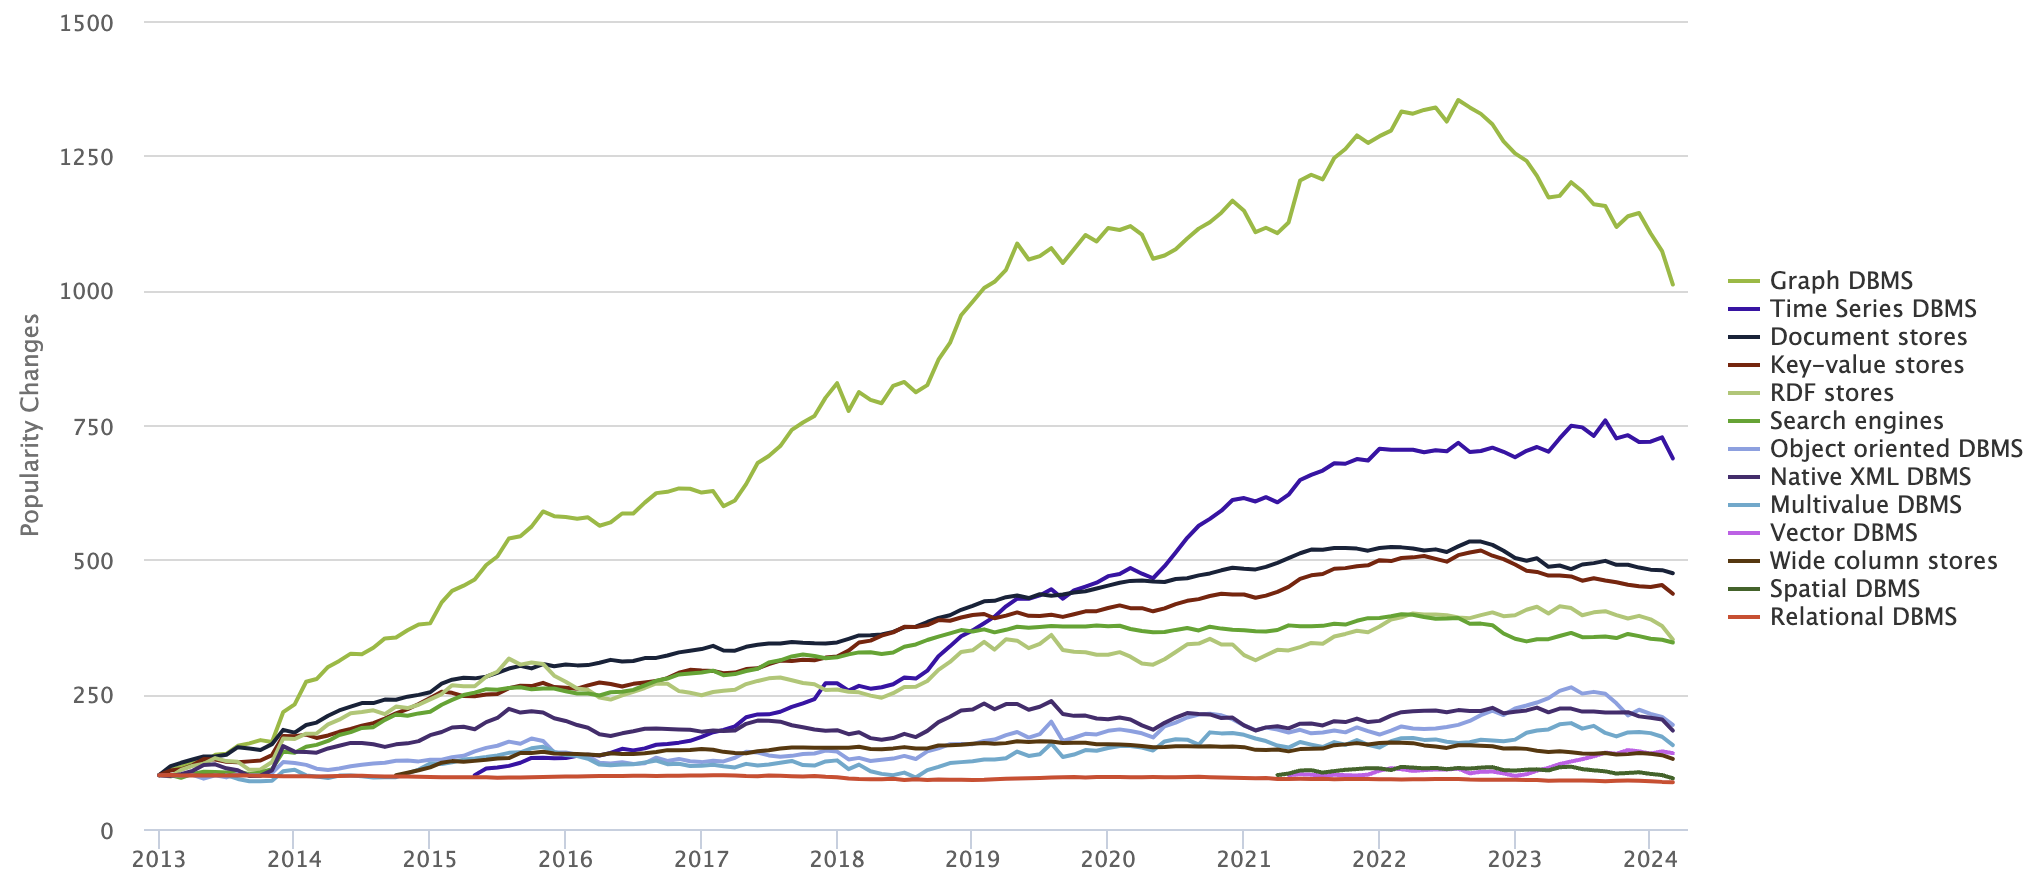
\includegraphics[width=\linewidth]{db-engines-ranking.png}
  \caption{DB-Engine 数据库类型流行度排名}
  \label{fig:db-engine}
\end{figure}

Apache IoTDB 是 Apache 基金会下一款开源的时序数据库,其具有为时间序列数据所优化的存储引擎、查询引擎以及分布式框架,可以满足工业物联网领域对海量时间序列数据高速写入、存储、快速读取以及复杂查询的需求\cite{wang2023apache}。

针对工业物联网场景下大量时序数据高速写入的需求,Apache IoTDB 主要提供了三种类型的数据写入接口:SQL 写入、原生列式写入接口、原生行式写入接口。在写入性能上,原生列式写入接口的性能最优,原生行式写入接口次之,SQL 写入性能最差;在写入的灵活性上,SQL 写入的灵活性最高,原生行式写入接口的灵活性次之,原生列式写入接口的灵活性最差。在大部分用户的使用场景中,SQL 式写入性能难以满足要求,原生列式写入接口则灵活性不足,使用原生行式写入接口可以兼具灵活性和良好的性能。但是,随着时序数据体量越来越大,原生行式接口写入较列式写入性能较差的问题显得越来越重要。例如,长安汽车车联网项目的一期工程有 12 亿条时间序列,采样周期为 30 秒,而二期工程不仅有 80 亿条时间序列,采样周期也减小到了 10 秒。如果原生行式写入接口的性能不变,粗略估计二期工程的服务器硬件成本约为一期的 20 倍。如果可以重新设计和实现一套高性能的行式写入机制,在负载相同的情况下就可以帮助用户降低机器的硬件成本,在负载越大的场景降成本的效果就越明显。设计和实现一套高性能的行式写入机制需要对客户端、网络传输、存储引擎等组件进行精心的设计和细致的优化。因此,提高 IoTDB 行式写入的性能具有一定的挑战性以及重要的实际意义和应用价值。
\section{Apache IoTDB 现有行式写入接口分析}
\subsection{Apache IoTDB 行式写入接口定义}
在 Apache IoTDB 中,时间序列采用树形的元数据结构进行描述。例如,某条时间序列可以被描述为 root.sg.d.s1,该字符串由多个“.”分隔开,“.”之间的字符则为元数据树中的一个节点。一条时间序列都倒数第二个节点被称为一个设备(Device),例如在前面的例子中 root.sg.d 就是一个设备。如果两个或多个时间序列都设备相同,那么则称这些时间序列是同一个设备下的序列。在大部分用户建模的场景中,设备通常对应了现实中的一个实体,例如一台机器或者一辆汽车,而设备下的每条序列则对应实体上部署的传感器。

IoTDB 提供的原生行式写入接口为 insertRecord 和 insertRecords,前者一次发送一行记录,而后者一次发送多行记录。为了减少由于网络传输带来的开销,大部分用户选择使用后者进行写入,本文所关注和研究的对象也主要是后者,即一次发送多行记录的写入形式。以 IoTDB 的 Java 客户端为例,insertRecord 和 insertRecords 接口的定义为:
\begin{lstlisting}[language=java,frame = trBL , firstnumber = last , escapeinside={(*@}{@*)}]
  void insertRecord(
      String deviceId,
      long time,
      List<String> measurements,
      List<TSDataType> types,
      List<Object> values
      )

  void insertRecords(
      List<String> deviceIds, 
      List<Long> times, 
      List<List<String>> measurementsList, 
      List<List<TSDataType>> typesList, 
      List<List<Object>> valuesList
      )
\end{lstlisting}
insertRecord 一次发送一行记录,这里的一行记录指的是这些数据属于一个设备下的时间序列,并且这些数据的时间戳都是相同的。表 \ref{tabular:insert-record-params} 详细介绍了该接口每个参数的含义。
\begin{table}
  \centering
  \caption{insertRecord 参数说明}
  \begin{tabular}{lll}
    \toprule
    参数名 &  类型 & 描述 \\
    \midrule
    deviceId & String & 数据所属的设备 ID \\
    time & long & 数据的时间戳 \\
    measurements & List<String> & 每个数据点所属的时间序列 ID 组成的列表 \\
    types & List<TSDataType> & 每个数据点所对应的数据类型 \\
    values & List<Object> & 每个数据点的数据 \\
    \bottomrule
  \end{tabular}
  \label{tabular:insert-record-params}
\end{table}

insertRecords 接口实际上是把多行记录一起从客户端发送到服务器,从接口的定义上看,每个与 insertRecord 接口对应的参数都变成了对应的列表,列表中的一个元素就描述了对应记录的相关信息,例如 deviceIds 中的每个元素就是每行记录对应的设备 ID。表\ref{tabular:insert-records-params} 中描述了 insertRecords 每个参数的含义。

\begin{table}
  \centering
  \caption{insertRecords 参数说明}
  \begin{tabular}{lll}
    \toprule
    参数名 &  类型 & 描述 \\
    \midrule
    deviceIds & List<String> & 每行记录所属的设备 ID 组成的列表 \\
     times & List<Long> & 每行记录的时间戳组成的列表 \\
    measurementsList & List<List<String> > & 每行记录的序列 ID 列表组成的列表 \\
    typesList & List<List<TSDataType> > & 每行记录数据类型列表组成的列表 \\
    valuesList & List<List<Object> > & 每行记录值列表组成的列表 \\
    \bottomrule
  \end{tabular}
  \label{tabular:insert-records-params}
\end{table}

综上,IoTDB 原生行式写入接口可以一次写入若干行记录,每条记录包含一个设备在一个时间戳下一条或若干条时间序列的数值。
\subsection{Apache IoTDB 现有行式写入机制实现}
\subsection{Apache IoTDB 现有行式写入机制不足}

\section{研究内容}
结合 \ref{sec:chap1-sec1} 和 \ref{sec:chap1-sec2} 节的分析,本文有以下发现:
\begin{enumerate}
  \item 在 Apache IoTDB 提供的三种写入接口中,原生行式写入接口具有较好的性能和灵活度,在大部分用户的场景下都适合适用。但是由于行式写入接口与列式写入接口具有一定的性能差距,在时间序列量较大的情况下无法满足用户的性能需求,也没有将服务器的资源高效利用。
  \item 
\end{enumerate}
\section{研究贡献}
\section{本文的组织结构}
% !TeX root = ../thuthesis-example.tex

\chapter{相关研究综述}
本节首先介绍目前主流时序数据库的写入接口设计,然后介绍与数据库客户端以及 RPC 优化有关的工作。
\section{时序数据库数据写入接口概述}
在目前市面上流行的时序数据库有四种常见的数据写入方式:SQL 写入、原生接口写入、行协议写入以及通过数据通信协议写入。下面将分别介绍这四种写入方式的特点。
\subsection{SQL 写入}
这种方式就是通过 SQL 语句进行写入,根据写入数据数据量的不同,又可以分为单行写入、多行写入和多表写入。应用需要先将写入数据的表名以及数据本体转换为 SQL,再通过 JDBC、ODBC 或者数据库的客户端执行 SQL。具有这一类写入接口的时序数据库有 Apache IoTDB、InfluxDB、TDEngine 等,目前 Apache IoTDB 支持单行写入和多行写入,InfluxDB 和 TDEngine 则支持单行写入、多行写入和多表写入。

对于用户而言,使用 SQL 写入最符合直觉,SQL 也是用户和所有数据库交互的一种通用方式。从开发者的角度来说,SQL 是一种和编程语言无关的交互协议,在为数据库开发不同编程语言下的客户端时,使用 SQL 进行写入可以避免对不同编程语言下数据结构的适配,减少开发时的工作量,提高开发效率。

然而,SQL 本身是一种文本,服务器在接收到 SQL 请求以后需要通过词法解析、语法解析等流程从 SQL 中提取出有效的信息,才能进行下一步的写入操作。而对 SQL 的解析需要消耗较多的 CPU,因此从资源利用的角度来说并不高效。因此,Apache IoTDB 在官方文档中明确推荐用户使用原生写入接口以提高写入性能\cite{iotdb2024javanative},InfluxDB 也在其官方教程中推荐用户使用行协议写入以提高性能\cite{influx2024highperformance}。TDEngine 将 SQL 写入作为推荐用户使用的写入方式之一,但是为了避免 SQL 解析对服务器资源的挤占,写入 SQL 会先在客户端进行解析,只有解析出来的结果才会发送到服务器执行写入。此外,从功能性的角度来说,SQL 语句只能传递数值类型、布尔类型和文本类型的数据,对于时序场景有可能存在的字节流数据、图片数据等非结构化数据则并不友好。
\subsection{原生接口写入}
这种写入方式通过特定的数据结构而不是 SQL 来传输需要写入的数据。相比于 SQL 式写入,原生接口写入将更多的信息直接传递给了服务器,不需要服务器从 SQL 提取有效的信息。然而,不同进程之间的数据结构不能直接传输,一般需要在客户端侧先序列化成二进制数据然后才能传输,服务器接收到二进制数据之后再反序列化为原本的数据结构,然后执行后续的写入步骤。

Apache IoTDB 提供了 \emph{insertTablets} 和 \emph{insertRecords} 两类同步原生写入接口,上层应用分别以 Tablet 和 Records 两种数据结构将数据传递给 SDK,然后 SDK 会调用 Apache Thrift\cite{apache2024thrift} 将数据序列化以后传输到服务器。Apache HoraeDB 提供了 Point 写入接口,每个数据点封装成 Point 的形式,然后一批数据点组成一个 Point 列表传递给写入 SDK。SDK 接收到 Point 列表以后会进行一系列的校验工作,然后使用 ProtocolBuffer\cite{currier2022protocol} 将数据序列化后传输到服务器。

使用原生接口写入的好处是将信息直接以数据结构的形式传递给服务器,服务器无需从 SQL 文本中推测数据的信息即可进行写入。在将数据结构序列化为二进制数据时,也可以根据数据类型的不同进行压缩和编码等优化,减少需要传输到数据量。SQL 等文本协议虽然也可以进行压缩,但是这些协议缺少了对数据类型、数据分布的先验知识,完全把数据当作文本进行压缩,因此效果不如原生接口写入。从这个角度看,原生接口写入在性能上具有天然的优势。王晨等人的工作也表明,Apache IoTDB 在使用 \emph{insertTablet} 接口时不仅写入延迟显著低于使用行协议写入的 InfluxDB,写入吞吐也要显著高于 InfluxDB\cite{wang2023apache}。此外,从功能性上来看,原生接口写入不仅可以方便地传递数值、文本和布尔类型的数据,对于字节流或者图片等结构化数据也有较好的支持。例如,国内某卫星发射基地使用 Apache IoTDB 的 \emph{insertRecords} 接口存储卫星发射观测过程中所产生的原始信号数据,如果使用文本类型的协议则无法很好地描述此类数据。

然而,原生接口写入也具有一些缺点。用户在使用原生接口写入时,往往需要了解写入 SDK 对数据结构的定义,然后将数据转换为 SDK 所需的数据结构,这样对应用侧带来了一些负担。其次,对于开发者来说,不同编程语言的数据结构之间有较大的差别,因此需要为不同编程语言下的客户端开发不同的 SDK,这增加了开发的工作量,也更容易产生软件缺陷。

\subsection{行协议写入}
行协议(Line Protocol)\cite{influx2024lineprotocol}是一种基于文本的写入协议,其中规定了数据写入的格式。例如 InfluxDB 所采用的 InfluxDB 行协议格式为\emph{measureable,metadata1,metadata2 <specific\_field>=<value>}。常见的行协议有 InfluxDB 行协议、OpenTSDB 行协议、Prometheus 行协议等。使用这一类行协议进行写入的数据库有 InfluxDB、OpenTSDB、TDEngine 等。

从本质上来说,行协议与 SQL 类似,都将需要写入的数据格式化到文本中,所以理论上行协议只是一种时序数据领域方言化的广义 SQL。但是,行协议是针对时序数据写入而设计的,所以一方面其在格式上相比 SQL 更加简洁,在解析过程中的开销相对较小;另一方面其能更加方便地描述时序数据的标签(Tag)、字段(Field)等信息,对于时序数据的特点有更好的支持。在 InfluxDB 的官方文档中提到,使用行协议写入具有如下优点:
\begin{enumerate}
  \item 通过网络传输到数据量更小,可以提高性能和节省成本;
  \item 数据更加易于探索(Explorable),可以更加方便地进行数据分析;
  \item 磁盘写入稍微更快,行协议的设计支持更高效的磁盘写入操作。
\end{enumerate}
此外,使用行协议进行数据写入也具有与 SQL 类似的通用性,不同编程语言 SDK 的开发工作量也相对较小。

使用行协议的具有以下几个缺点。首先,相较于原生接口写入,行协议仍然要求服务器从文本中提取出写入所需要的信息,这一过程会带来一定的开销。其次,行协议是一种文本协议,对于字节流、图片等非结构化数据的写入并不友好。最后,用户在使用行协议写入时可能需要一定都学习成本,因为其并不如 SQL 那样直观。为了解决最后一个缺点,InfluxDB 等数据库推出了一些客户端工具,如 Telegraf\cite{influx2024telegraf},这些工具对行协议进行了一定的封装,让用户可以以更加直观的方式进行写入。

\subsection{通过数据通信协议写入}
在这种写入方式中,客户端将数据通过常见的数据通信协议进行打包和发送,服务器接收到数据后进行解包和写入。在物联网场景中,常见的数据通信方式有 OPC 协议\cite{zheng2002opc}、MQTT 协议\cite{soni2017survey}、RESTful API 协议\cite{fielding2000architectural} 等。

OPC 协议的全称为 OLE for Process Control,是一种工业通信标准,旨在促进不同制造商的自动化设备、系统和软件之间的数据交换和互操作性。OPC 标准由 OPC Foundation 维护,该组织由多个硬件制造商、软件开发商和系统集成商组成,共同推动和支持这一开放的、独立于平台的通信标准。OPC 有多个版本,其中 OPC UA(Univerised Architecture)是最新的 OPC 通信标准,具有跨平台、加密安全、按需访问等特性\cite{hannelius2008roadmap},图 \ref{fig:opc-arch} 展示了 OPC 通讯协议的架构图。 在 OPC UA 协议中存在一个 OPC UA Server 的角色,它提供订阅功能,负责进行数据的交换。时序数据库可以向 OPC UA Server 订阅需要写入的时间序列,数据产生后先从客户端上被发往 OPC UA Server,OPC UA Server 再将接收到的数据发送到时序数据库进行写入。
\begin{figure}
  \centering
  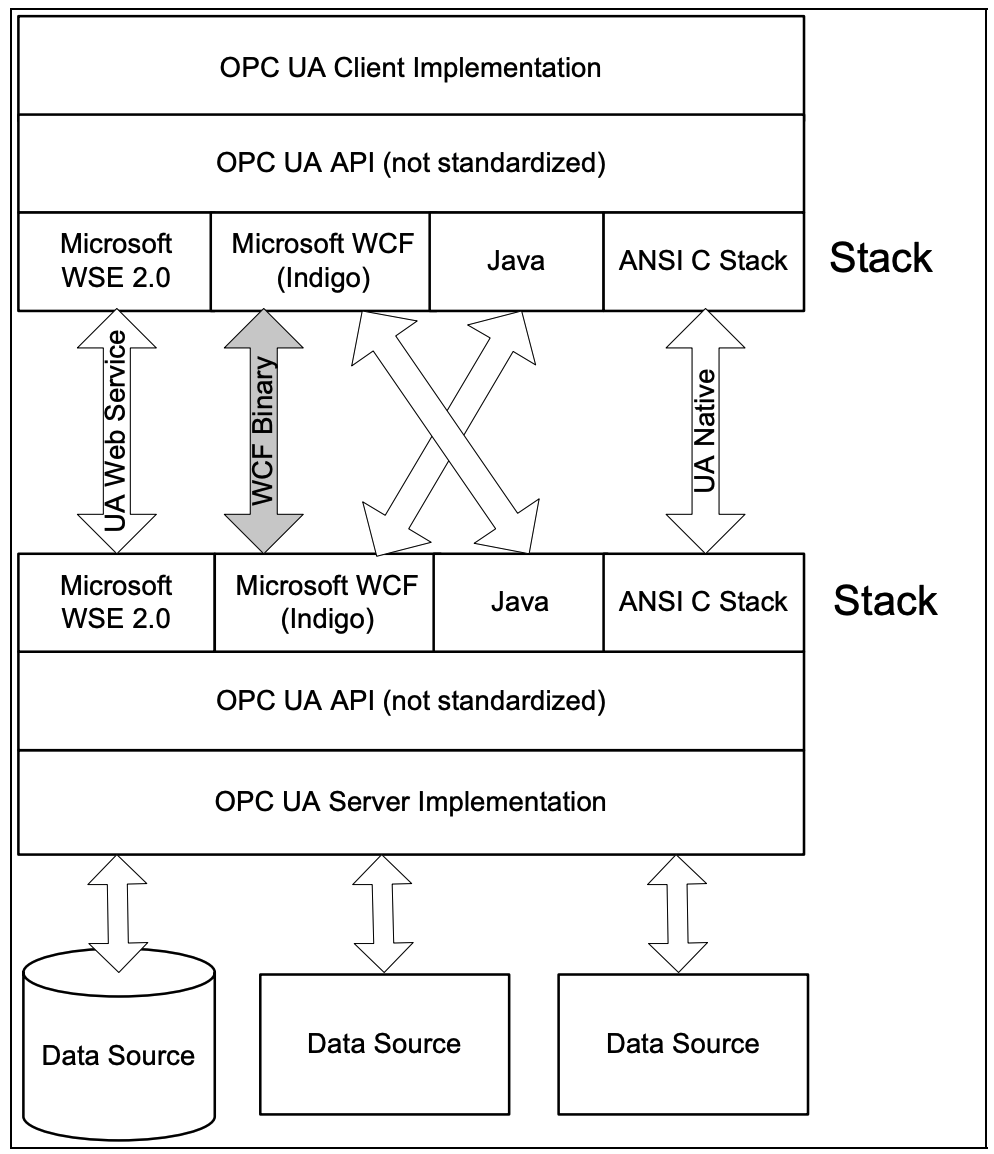
\includegraphics[width=0.8\textwidth]{OPC-UA-arch.png}
  \caption{OPC UA 通讯架构图\cite{leitner2006opc}}
  \label{fig:opc-arch}
\end{figure}


MQTT 协议的全称为 Message Queuing Telemetry Transport,是一种轻量级的、基于发布/订阅模型的消息传输协议,它专为低带宽、高延迟或不可靠的网络环境设计。MQTT 协议因其设计简洁、占用资源少、通信效率高而广泛应用于物联网、移动应用程序、车载系统和智能家居等场景\cite{yassein2017internet}。图 \ref{fig:mqtt-arch} 展示了使用 MQTT 通讯时的架构图。当数据使用 MQTT 协议写入时,客户端将采集到的数据发送到 MQTT 服务器,MQTT 服务器再将数据发送到对应的订阅者,时序数据库可以作为订阅者接收到数据后进行写入。
\begin{figure}
  \centering
  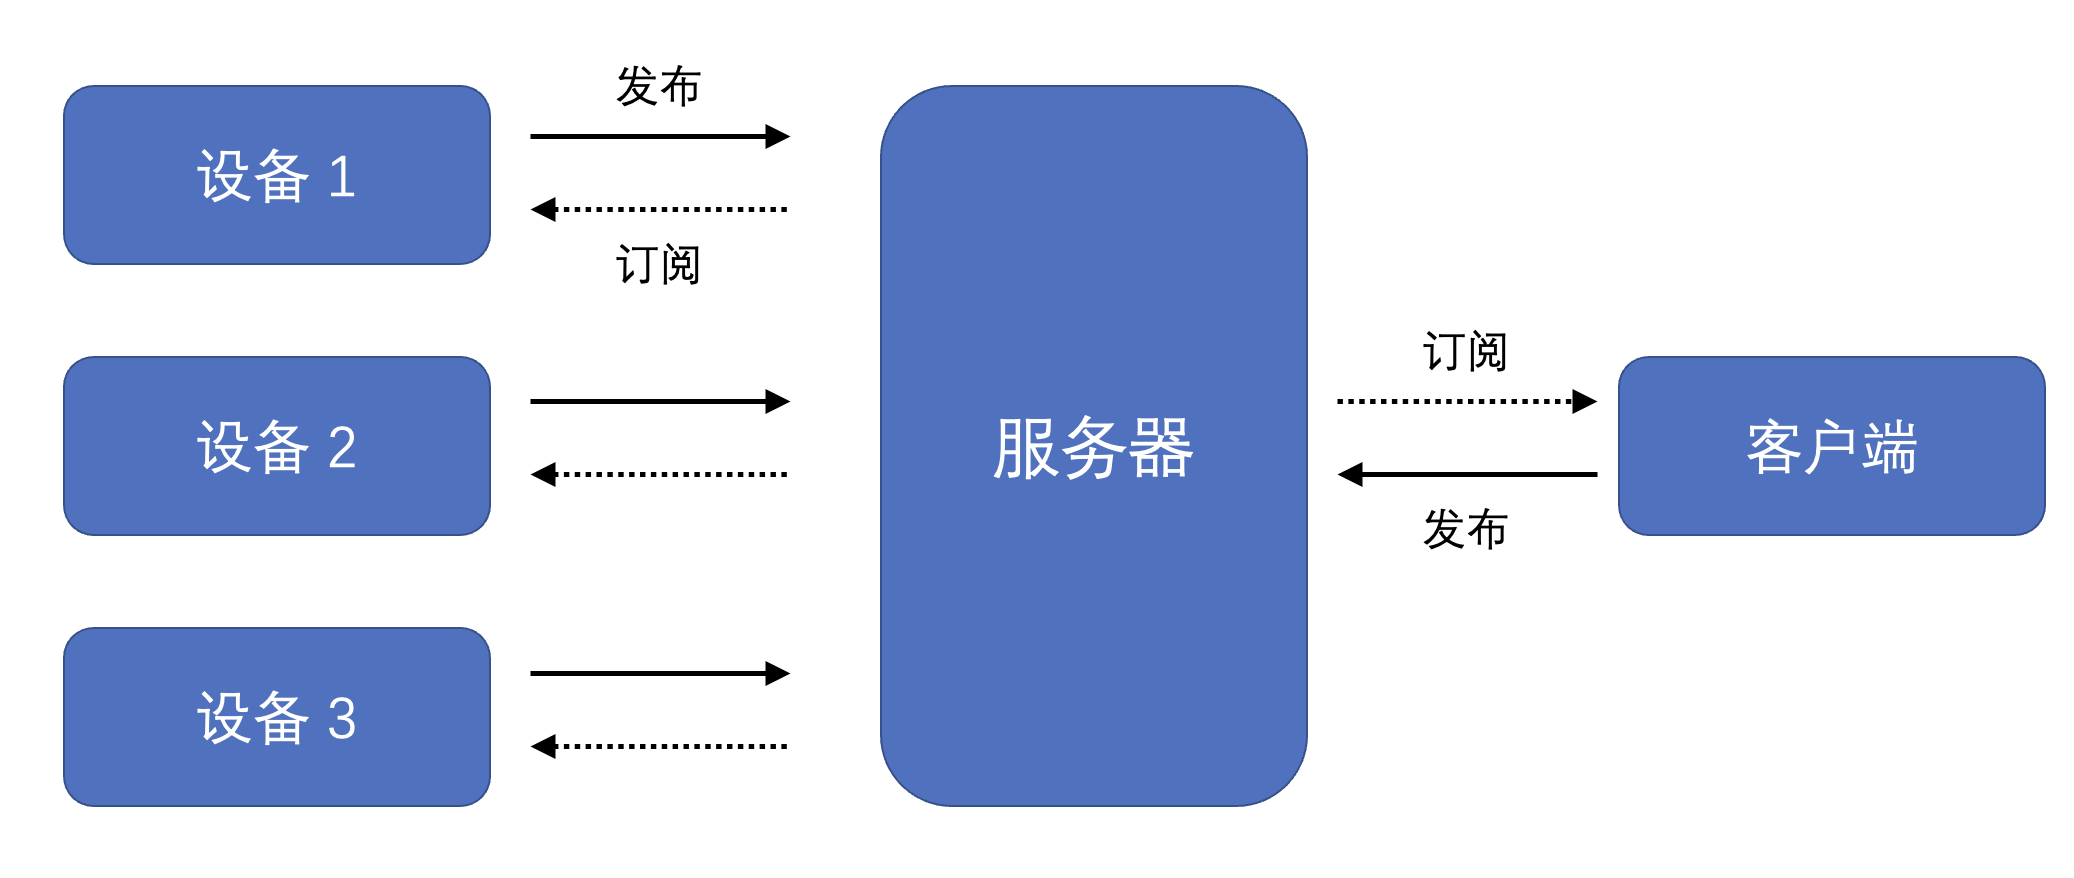
\includegraphics[width=0.8\textwidth]{mqtt-arch.png}
  \caption{MQTT 通讯架构图\cite{soni2017survey}}
  \label{fig:mqtt-arch}
\end{figure}

RESTful API 的全称是 Representational State Transfer API,指的是一种遵循 REST 风格的 API。RESTful API 通过使用 HTTP 协议的标准方法(如GET、POST、PUT、DELETE)来创建、读取、更新和删除资源,实现客户端和服务器之间的交互。在使用 RESTful API 写入时,客户端通常会向服务器发送一个 POST 请求,并且将需要写入的数据放到 POST 请求的 body 中,服务器接收到请求后解析 body 中的数据,然后进行写入。

在目前主流的时序数据库中,Apache IoTDB 和 InfluxDB 都支持以上三种通讯方式进行数据写入;TDEngine 目前仅支持 RESTful API 写入,但是其官方文档中也提到了未来会支持 MQTT 协议和 OPC 协议写入;Prometheus 目前仅支持 RESTful API 写入,但是有一些第三方开发者为 Prometheus 提供了 MQTT 和 OPC 支持;Apache HoraeDB 则对以上三种写入方式都不支持。

使用这些通信方式进行数据写入有以下几个优点。首先,这些通讯方式的应用比较广泛,市面上存在大量成熟的通讯库可以直接调用,降低了开发者的开发成本。其次,这些通讯方式也对数据的格式没有太大限制,可以方便地传输结构化数据、半结构化数据以及非机构化数据。最后,这些通讯方式也非常灵活,开发者甚至无需使用数据库的 SDK 就可以直接向数据库中写入数据。

使用这样的数据写入方式也存在着一些弊端。首先,这些通讯方式本身并不是为了高性能场景而设计的,因此在性能上可能不如原生接口写入和行协议写入。其次,因为这些协议是为了通用场景而开发的,通过这些协议进行写入时存在的性能优化空间也比较小。因此,大部分使用这些协议的场景都是在数据量较小、写入频率较低的场景下。


\section{数据库客户端与数据序列化优化\label{sec:chap2-sec3}}
基于客户端-服务器(Client-Server,CS)架构的数据库几乎都实现了一套自己的客户端协议,其承担着向服务器发送查询/写入请求,接收服务器查询/写入结果的作用,其性能是决定数据库整体性能的关键一环。常见的客户端协议实现有对 JDBC\cite{zukowski2006jdbc} 和 ODBC\cite{geiger1995inside} 接口的实现。为了保持对已有数据库的兼容性,一些数据库系统选择复用现有的数据库客户端协议,例如 RedShift\cite{gupta2015amazon}、Greenplum\cite{lyu2021greenplum}、Vertica\cite{lamb2012vertica}、Hyper\cite{neumann2011efficiently} 都选择实现了 PostgreSQL 的客户端协议,Spark SQL\cite{armbrust2015spark} 选择实现了 Hive 的客户端协议。总之,目前市面上存在着许多不同的客户端协议。

客户端协议的设计是一个需要权衡的问题:如果选择使用激进的压缩和序列化技术,虽然可以减少通过网络传输的数据量,但是会增加序列化和反序列化的时间;如果选择使用保守的客户端协议,虽然会减少序列化和反序化的耗时,但是需要通过网络传输的数据增加了,这会增加网络传输的延迟。Raasveldt 等研究了常见数据库在 TPC-H 数据集\cite{poess2000new}下,对 lineitem 表进行全量查询时查询过程的耗时分布,发现大部分数据库所使用的客户端协议并不高效,占据了整个查询过程中的大部分耗时。随后,他们分析了各类客户端协议的设计以及客户端协议的设计空间(Design Space),最后提出了一个列式的客户端协议,降低了查询的延迟\cite{raasveldt2017don}。

Galakatos 等认为在具有 RDMA(Remote Direct Memory Access)\cite{recio2007remote}能力的网络环境下,传统分布式数据库的通信协议无法有效利用网络的全部能力。他们为 OLTP 数据库、OLAP 数据库以及高级分析框架重新针对 RDMA 环境设计了新的架构,以更好地利用 RDMA 的能力,实验结果表明重新设计后的系统性能有较大提升\cite{galakatos2016end}。

Wang 等针对高级分析框架从数据库中读取数据这一场景,分析了已有客户端加载速度慢、耗费内存巨大的原因,同时设计了一个简洁的领域特定语言(Domain Specific Language,DSL)来映射数据库查询结果到数据框架中的数据表示,并在其中使用了并行执行、字符串分配优化和高效数据表示等优化技术,成功地提高了数据分析任务执行过程中数据加载的效率\cite{wang2022connectorx}。

Durner 等针对云环境设计了一个名为 Crystal 的存储系统,其中的存储层和计算层是相互解耦的。为了提高系统在使用远程存储时的性能, Crystal 的客户端是带有下推谓词的特定于 DBMS 的“数据源”。实验结果表明,这种设计可以显著改善查询延迟,同时还节省了来自远程存储的带宽\cite{durner2021crystal}。

以上这些工作是目前学术界和工业界对客户端设计和协议优化的一些研究,但是这些研究大部分集中在数据查询和数据科学场景,对于大批量的数据(尤其是时序数据)的写入则缺少关注。
% !TeX root = ../thuthesis-example.tex

\chapter{IoTDB 现有写入机制介绍与分析}
本章首先介绍 Apache IoTDB 目前已有的 \emph{insertRecords} 和 \emph{insertTablet} 接口,随后介绍 \emph{insertRecords} 写入接口执行的全部流程,包括客户端侧的数据封装、RPC 层的数据序列化与反序列化、存储引擎侧写入内存表以及最终持久化的过程。最后使用 IoT Benchmark 对 \emph{insertRecords} 接口进行性能测试和分析,找出目前 \emph{insertRecords} 接口性能不如预期的原因,为本文后续设计新 \emph{insertRecords} 写入机制提供参考。
\section{IoTDB 现有写入接口}
在 \ref{sec:chap1-sec1} 和 \ref{sec:chap1-sec2} 节中,我们简要介绍了 Apache IoTDB 现有的 \emph{insertRecords} 接口和 \emph{insertTablet} 接口,以及它们运行的整体流程。在本节中我们将进一步深入讨论 \emph{insertTablet} 和 \emph{insertRecords} 接口的设计以及两者在不同场景下的适用情况。

\subsection{Apache IoTDB 写入接口形式}
目前 IoTDB 主要提供了四种原生写入接口,分别是 \emph{insertRecord}、\emph{insertRecords}、\emph{insertTablet}、\emph{insertTablets}。这四种接口中 \emph{insertRecords}、\emph{insertTablet}、\emph{insertTablets} 都是批量化的写入接口,只有 \emph{insertRecord} 一次只写入一条记录。由于批量化写入可以将写入过程中的一些固定代价均摊到多个数据点上,可以减少写入总体代价\cite{bercken2001evaluation},因此 \emph{insertRecord} 的性能远不如其他三个接口,在生产环境中也几乎没有用户使用。以 IoTDB 的 Java SDK 为例,它们的接口定义如下:
\begin{lstlisting}[language=java,frame = trBL , firstnumber = last , escapeinside={(*@}{@*)}]
  void insertRecord(
      String deviceId,
      long time,
      List<String> measurements,
      List<TSDataType> types,
      List<Object> values
      )

  void insertRecords(
      List<String> deviceIds, 
      List<Long> times, 
      List<List<String>> measurementsList, 
      List<List<TSDataType>> typesList, 
      List<List<Object>> valuesList
      )

  void insertTablet(Tablet tablet)

  void insertTablets(Map<String, Tablet> tablets)
\end{lstlisting}
其中,Tablet 是一个数据结构,代表一个设备的一批数据,其结构如下:
\begin{lstlisting}[language=java,frame = trBL , firstnumber = last , escapeinside={(*@}{@*)}]
public class Tablet {
  public String deviceId;
  private List<MeasurementSchema> schemas;
  public long[] timestamps;
  public Object[] values;
  public int rowSize;
}
\end{lstlisting}
\emph{insertRecord} 和 \emph{insertRecords} 的参数含义则如表 \ref{tabular:insert-record-params} 和表 \ref{tabular:insert-records-params} 所示,\emph{Tablet} 的成员变量含义如表 \ref{tabular:class-tablet-param} 所示。
\begin{table}
  \centering
  \caption{insertRecord 参数说明}
  \begin{tabular}{lll}
    \toprule
    参数名 &  类型 & 描述 \\
    \midrule
    deviceId & String & 数据所属的设备 ID \\
    time & long & 数据的时间戳 \\
    measurements & List<String> & 每个数据点所属的时间序列 ID 组成的列表 \\
    types & List<TSDataType> & 每个数据点所对应的数据类型 \\
    values & List<Object> & 每个数据点的数据 \\
    \bottomrule
  \end{tabular}
  \label{tabular:insert-record-params}
\end{table}

\begin{table}
  \centering
  \caption{insertRecords 参数说明}
  \begin{tabular}{lll}
    \toprule
    参数名 &  类型 & 描述 \\
    \midrule
    deviceIds & List<String> & 每行记录所属的设备 ID 组成的列表 \\
     times & List<Long> & 每行记录的时间戳组成的列表 \\
    measurementsList & List<List<String> > & 每行记录的序列 ID 列表组成的列表 \\
    typesList & List<List<TSDataType> > & 每行记录数据类型列表组成的列表 \\
    valuesList & List<List<Object> > & 每行记录值列表组成的列表 \\
    \bottomrule
  \end{tabular}
  \label{tabular:insert-records-params}
\end{table}

\begin{table}
  \centering
  \caption{Tablet 类成员变量含义说明}
  \begin{tabular}{llp{6cm}}
    \toprule
    参数名 &  类型 & 描述 \\
    \midrule
    deviceId & String & 该 Tablet 所属的设备 ID \\
    schemas & List<MeasurementSchema> & 该 Tablet 中每个测点的元数据信息 \\
    timestmaps & long 类型数组 & 该 Tablet 中每一行数据的时间戳 \\
    values & Object 类型数组 & 该 Tablet 中每一个测点的数据,其中的每一个对象都代表一列数据 \\
    rowSize & int & 该 Tablet 中包含的数据行数\\
    \bottomrule
  \end{tabular}
  \label{tabular:class-tablet-param}
\end{table}

从接口形式上看,\emph{insertRecords}、\emph{insertTablet} 和 \emph{insertTablets} 其实都是在不同维度上进行批量化的写入接口:
\begin{itemize}
  \item \emph{insertRecords} 一次性可以写入多行数据,每一行数据都是任意一个设备在同一个时间戳下若干个测点的数据,不同行之间可以是不同的设备在不同时间戳下的数据。从这一点看,\emph{insertRecords} 是在多设备、多时间戳维度上进行批量化的写入接口。
  \item \emph{insertTablet} 一次写入一个 Tablet,每个 Tablet 只能包含一个设备在不同时间戳下的数据,不同设备的数据无法共享一个 Tablet。因此,\emph{insertTablet} 是对同一个设备在多时间戳维度上进行的批量化写入。
  \item \emph{insertTablets} 一次可以写入多个 Tablet,每个 Tablet 包含一个设备在不同时间戳下的数据。因此,\emph{insertTablets} 其实也是在多设备、多时间戳维度上进行批量化的写入接口。
\end{itemize}
\emph{insertRecords} 接口和 \emph{insertTablets} 接口在批量化的维度上是相同的,因此理论上使用 \emph{insertRecords} 接口的场景都可以使用 \emph{insertTablets},反之亦然。然而,由于 \emph{insertTablets} 接口要求用户先将需要写入的数据按照设备归类并封装成 Tablet 结构体,对于用户而言使用复杂度较高,\emph{insertRecords} 对数据形式的要求则更低,因此使用 \emph{insertRecords} 的用户数更多。
\subsection{不同写入接口的性能对比\label{sec:chap3-sec1-1}}
但是这两者在数据结构上有所不同。在 \emph{insertRecords} 中,属于同一个设备的数据可能会分布在不同的位置;在 \emph{insertTablets} 中,属于同一个设备的数据会被集中在同一个 Tablet 中。后一种模式能够在写入的后续处理流程中占有一些优势:数据在写入时首先进入内存表(MemTable)中,IoTDB 将同一个设备下的时间序列存储在内存表中的同一个块组(Chunk Group)中,如果同一个设备的数据都聚集在一起,那么就可以将它们一起写入到块组中,数据写入内存表的次数与 Tablet 的个数相同。而在 \emph{insertRecords} 的写入过程中,由于每一条 Record 都可能属于不同设备,因此只能一条一条 Record 地进行写入,写入内存表的次数与 Record 的数量相同,性能在某些情况下相比 \emph{insertTablets} 可能更低。

为了对比目前 \emph{insertRecords} 接口与 \emph{insertTablets} 的性能,笔者使用 IoTDB Benchmark\cite{liu2019benchmarking} 对 IoTDB 的 \emph{insertRecords} 和 \emph{insertTablets} 接口在不同的请求模式下进行测试。笔者固定单个写入请求的数据总行数为 400,调节单个请求中不同设备数,观察两种接口的性能变化\footnote{IoTDB 版本为 1.3.0,实验环境 CPU 为 I7-11700,DataNode 使用 28GB 内存,ConfigNode 2GB,硬盘为 HDD}。例如,如果一个请求中只有 1 个设备,那么一个请求中的 400 行都是该设备的数据;如果一个请求中有 10 个设备,那么请求中每个设备都各自有 40 行数据。图 \ref{fig:records-vs-tablets-throughput} 和图 \ref{fig:records-vs-tablets-latency} 分别展示了两种接口吞吐和延迟随设备数不同而出现的变化。

\begin{figure}
  \centering
  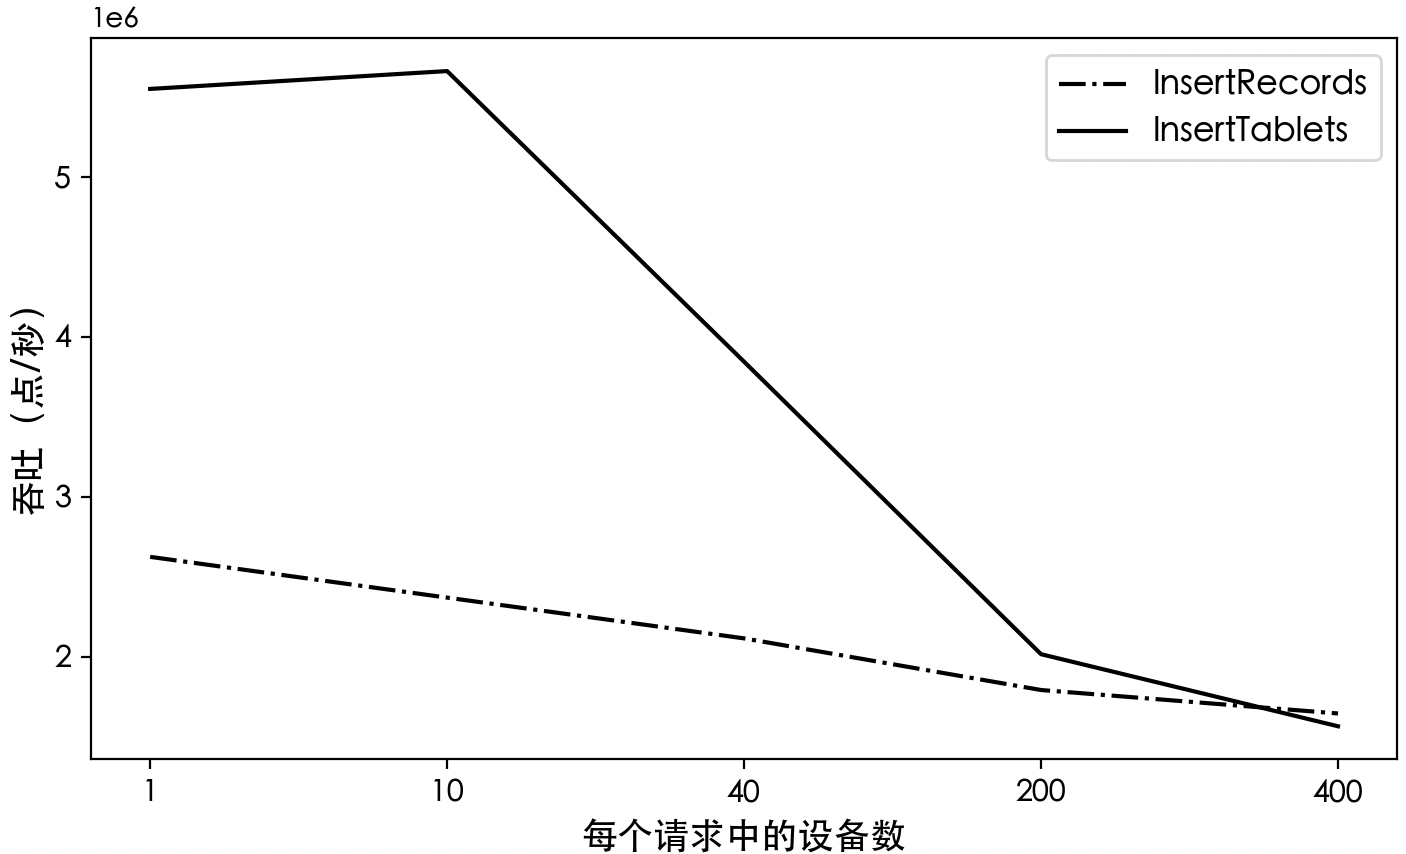
\includegraphics[width=\linewidth]{records-vs-tablets-throughput.png}
  \caption{一次写入请求中写入吞吐随设备数的变化}
  \label{fig:records-vs-tablets-throughput}
\end{figure}

\begin{figure}
  \centering
  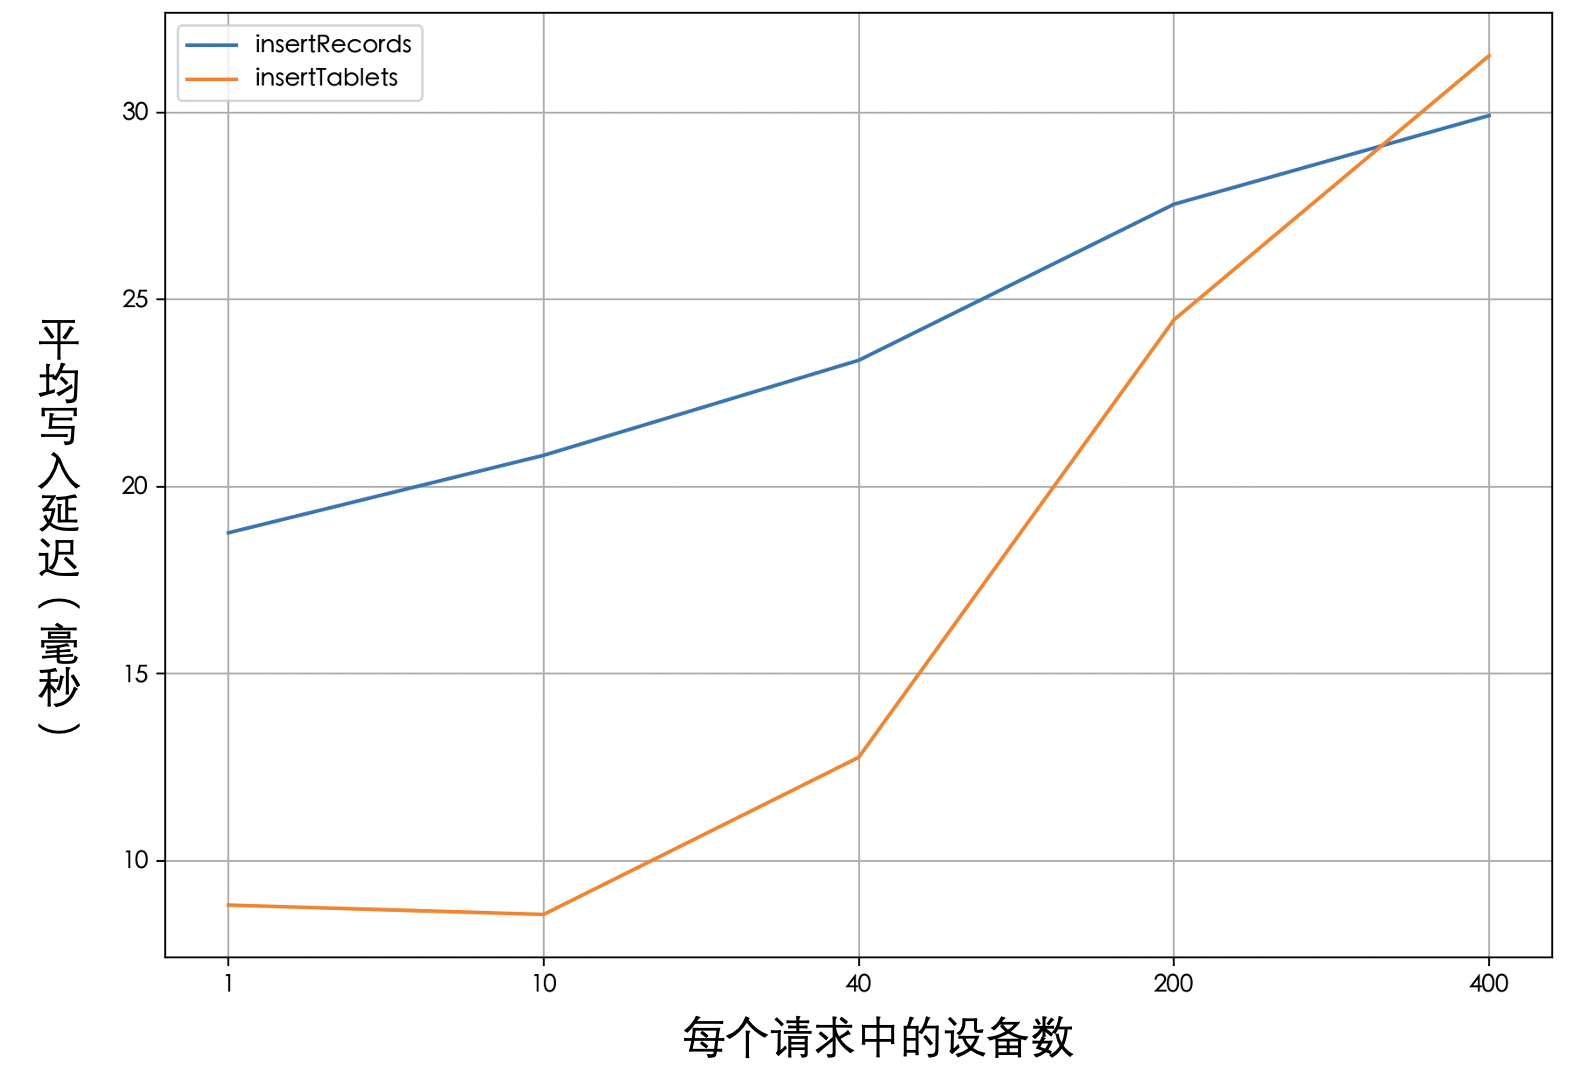
\includegraphics[width=\linewidth]{records-vs-tablets-latency.png}
  \caption{一次写入请求中写入延迟随设备数的变化}
  \label{fig:records-vs-tablets-latency}
\end{figure}

从实验结果中可以看出,当设备数小于 400,即每个设备都有超过 1 条数据时,\emph{insertTablets} 接口的性能要优于 \emph{insertRecords};当设备数等于 400 时,也就是每个设备在一次请求中都只有 1 条数据时,\emph{insertRecords} 接口要略微优于 \emph{insertTablets}。这个实验结论与上一节中对这两个接口的分析是一致的,使用 Tablet 写入可以利用同一设备的数据被提前聚集的特点进行批量化写入,实现较好的性能;而 \emph{insertRecords} 由于提前不知道同一设备数据的分布,只能一条一条地写入存储引擎,性能较差。当一个请求中每个设备都只有一条数据时,使用 \emph{insertTablets} 接口写入时每个 Tablet 都只有一行数据,此时其执行逻辑实际上和 \emph{insertRecords} 是差不多的。由于 \emph{insertRecords} 针对行式写入有一些优化,因此其性能略好于 \emph{insertTablets}。
\subsection{不同接口的使用场景}
\emph{insertRecords} 和 \emph{insertTablets} 接口在设备和时间两个维度进行了批量化,而 \emph{insertTablet} 接口则时间这个维度进行了批量化。不同批量化维度会导致不同接口的适用场景有所不同。

按照数据产生的频率进行划分,可以将时序数据写入的场景分为高频和中低频两种场景。在高频场景中,传感器的采样率很高,短时间内会产生大量时序数据,并且这些数据都属于同一个设备。例如在风力发电场景中风机上的传感器在某些情况下的采样频率可以达到 8KHz\cite{李天安2020apache},如果将一个风机建模为一个设备,并且假设传感器的采样频率一致,那么一个设备每秒钟就会产生 8000 行数据。在中低频场景中,传感器的采样频率较低,可能每隔几十秒传感器才会产生一个数据点。例如在长安汽车的车联网场景中,一辆汽车被建模为一个设备,汽车上的传感器每隔 30 秒才会进行一次采样,如果所有传感器的采样频率一致,那么一个设备每隔 30 秒才会产生一行数据。

数据产生频率的不同会导致这些场景适用不同接口。在高频场景中,由于一个设备的数据产生地非常快,使用 \emph{insertTablet} 或者 \emph{insertTablets} 接口可以充分利用数据按设备批量化的特点,将其快速写入到存储引擎中。如果使用 \emph{insertRecords} 接口,则无法利用每个设备下数据较多的特点,将数据一行一行地写入,导致最终性能不高。在低频场景中,数据间隔很久才会产生,如果使用 \emph{insertTablet} 或者 \emph{insertTablets} 接口就有两种选择:
\begin{enumerate}
  \item 为了提高写入性能,对数据进行缓存和积攒,等到 Tablet 的大小较大时才写入。但是这样会导致数据从产生到写入会经历非常长的时间。以长安汽车为例,一辆汽车被建模为一个设备,假如需要积攒到一个 Tablet 中有 100 行数据才写入,那么数据从产生到写入数据库的延迟为 50 分钟,在此期间其他应用无法从数据库中查询到这些数据,这是不可接受的。
  \item 为了及时写入数据,在每个 Tablet 较小时就进行写入。从上一节的实验结果中我们可以知道这样不仅无法发挥出 Tablet 写入的性能,对数据分 Tablet 进行组装还会对上层应用带来额外的复杂度。
\end{enumerate}
如果使用 \emph{insertRecords},可以令 Record 的数量积攒到一定程度以后一起发送给服务器进行写入,并且 \emph{insertRecords} 的接口形式更加直观,可以减轻用户侧的复杂度。因此,长安汽车在其业务中选择的就是 \emph{insertRecords} 接口进行数据写入。

但是,从 \ref{sec:chap3-sec1-1} 节中的实验结果不难发现,\emph{insertRecords} 接口虽然有着使用方便的优点,但是其性能与 \emph{insertTablets} 接口有一定的差距。因此,如果我们可以将 \emph{insertRecords} 写入接口的性能提升,那么对于用户而言既可以使用比较友好的接口,省去将数据归类为 Tablet 的繁琐过程,又可以获得不错的写入性能。所以,本文的研究重点是如何在保持 \emph{insertRecords} 接口不变的情况下,通过设计新的底层实现机制,实现高性能的 \emph{insertRecords} 写入。
\section{Apache IoTDB 中 \emph{insertRecords} 写入的实现}
在研究如何设计出新的 \emph{insertRecords} 写入实现机制之前,本文先介绍目前 Apache IoTDB 对 \emph{insertRecords} 写入机制的实现。从应用层调用 IoTDB SDK 提供的 \emph{insertRecords} 接口开始,写入会经历客户端侧的数据封装、RPC 层数据序列化与反序列化、存储引擎侧数据写入内存表以及内存表数据的持久化。下面将详细介绍这个过程。
\subsection{客户端侧的数据封装流程}
客户端在接收到用户传入的写入数据后,需要对数据进行校验、划分和封装,其操作如下:
\begin{itemize}
  \item \emph{insertRecords} 的每一个参数都是列表(List),在合法的语义下每个参数的长度应该相同,如果不同参数的列表长度不一致就需要停止写入并抛出错误。
  \item 经过校验之后,数据会进行分片。Apache IoTDB 是一个分布式的数据库,一个集群中可能存在多个数据节点。一条时间序列的数据会被切分成多片,分布在多个数据节点中\cite{wang2023apache}。用户通过接口传入的一批数据就可能需要写入不同的节点。为了更高效地写入,IoTDB 的客户端会缓存不同序列对应的数据节点地址,然后将传入的数据按照节点地址进行划分,写入同一个节点的数据集合成一个子请求。
  \item 每一个子请求都包含了用户写入的数据的若干行,包括这些行的设备 ID、时间序列 ID、数据类型、时间戳以及数据值。IoTDB 客户端在把数据交由 RPC 层进行传输前,会提前把数据类型以及数据值序列化为二进制数据。每一行序列化的格式都如图 \ref{fig:curr-line-serialize-format} 所示:首先序列化一个数据点的类型,然后是它的值,紧接着是下一个数据点的类型和值。一行数据序列化为一个字节流对象(ByteBuffer),一个请求中的多行数据序列化的结果是字节流对象的列表(List<ByteBuffer>),其中的每一个元素都代表了原来的一行数据。
\end{itemize}

\begin{figure}
  \centering
  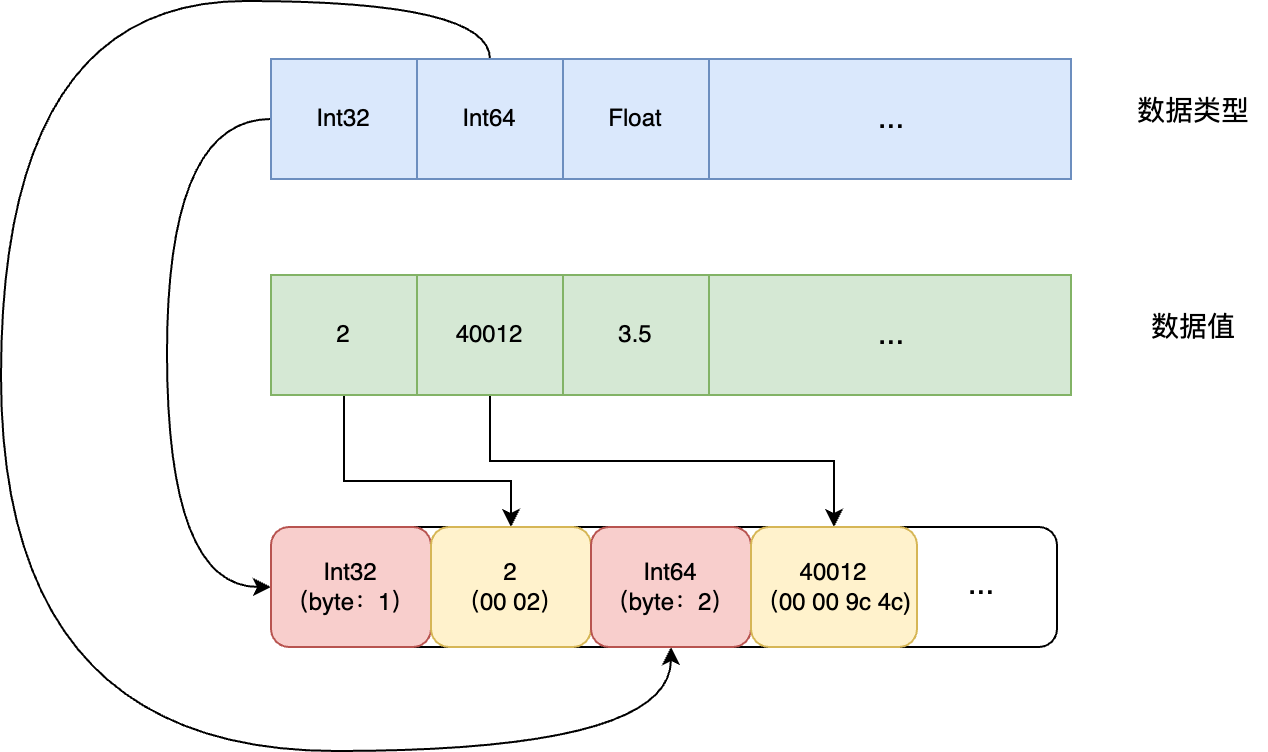
\includegraphics[width=\linewidth]{curr-data-serialize.png}
  \caption{一行数据序列化过程}
  \label{fig:curr-line-serialize-format}
\end{figure}

\subsection{RPC 层的数据序列化与反序列化流程}
\subsection{存储引擎侧数据写入内存表流程}
\subsection{存储引擎侧数据持久化流程}
\section{当前机制性能分析}
\section{本章小结}
% !TeX root = ../thuthesis-example.tex

\chapter{新 \emph{insertRecords} 写入机制总体设计}
本章介绍新 \emph{insertRecords} 写入机制的总体设计,包括客户端侧数据预处理、RPC 数据序列化格式设计、存储引擎批量并行化写入。

\section{新写入设计总览}
\begin{figure}
  \centering
  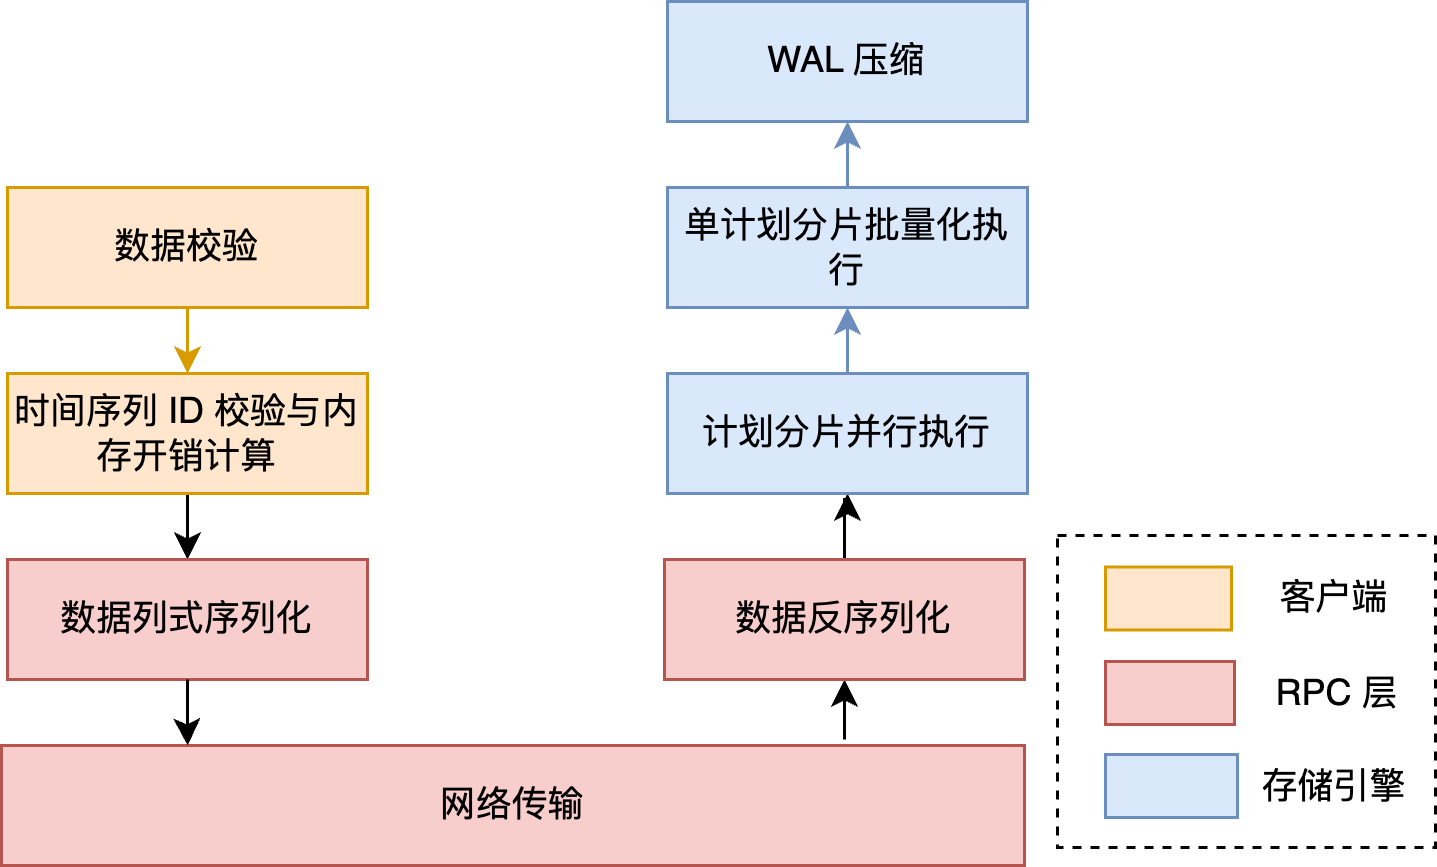
\includegraphics[width=\linewidth]{new-insert-records-overview.png}
  \caption{新 \emph{insertRecords} 写入机制}
  \label{fig:new-insert-records-overview}
\end{figure}

图 \ref{fig:new-insert-records-overview} 展示了新 \emph{insertRecords} 写入机制的总体设计。新写入机制有如下的设计目标:
\begin{enumerate}
  \item 提高系统性能:在相同的硬件下实现更高的写入性能,包括更高的吞吐以及更低的延迟;或者在相同的写入性能下降低对系统资源的使用;
  \item 提高系统整体资源的利用率:充分利用系统中客户端和服务器侧的计算、存储、网络资源,避免资源闲置;
  \item 具有高稳定性:在持续的高负载下系统应当能够保持较好的写入性能,避免出现剧烈的波动。
\end{enumerate}
为了实现这样的目标,新写入机制的总体设计思路为:
\begin{itemize}
  \item 存储引擎侧构建高效率的写入方式,将数据批量化、并行化写入,将写入过程中的固定开销尽量平摊到多条数据上,提高系统资源的利用率。
  \item 将服务器端的部分工作卸载(Offload)到客户端上,在客户端侧进行少量轻量级的计算,提高整体资源的利用率。
  \item 减少经过网络传输的冗余数据量,通过高效的列式数据格式提高网络资源的利用率。
\end{itemize}
本章的剩余内容从客户端、RPC 层、存储引擎三个方面简要介绍新 \emph{insertRecords} 写入机制的设计。

\section{客户端侧数据预处理}
在 \ref{sec:chap2-sec3} 节中,本文介绍了一些对于客户端进行优化的相关工作。其中, Crystal 存储系统基于远程存储所设计\cite{durner2021crystal}。因为数据通过远程存储设施进行读取的性能较差,所以为了提高系统的性能,Crystal 的客户端增加了谓词下推功能,被下推到数据源的谓词可以提前过滤掉一些不符合条件的数据,减少通过网络传输的数据量,提高系统的性能。在时序数据库中,TDEngine 的客户端也是“重客户端”设计的代表。TDEngine 的客户端不仅承担了对 SQL 进行解析的工作,还负责缓冲系统的元数据,在写入之前进行元数据校验。

目前 IoTDB 的客户端只负责数据的简单校验和传输,其余工作都由服务器承担。从系统的整体资源利用率的角度看,在目前的设计中 IoTDB 客户端侧的资源并没有被充分利用起来。因此,本文将服务器所承担的部分不依赖于已有数据的工作卸载到客户端侧。参考表 \ref{tabular:insert-records-profile-result} 可知,这一类工作中开销最大的就是时间序列 ID 和内存开销计算,本工作将会把这两项任务从服务器端移到客户端。

\section{RPC 层列式数据序列化格式}
IoTDB 是一个时序数据库,本质上是一个针对时序场景优化的 OLAP 数据库\cite{谭新宇2023一致性协议}。在 OLAP 数据库中提高系统性能的一个常见方式是将数据按照列的形式存储和处理。根据 \ref{sec:chap3-sec2} 的对目前 IoTDB \emph{insertRecords} 写入请求序列化的介绍可以知道,目前所使用的序列化方式是行式的。结合 \ref{sec:chap3-sec3-1} 节的实验结果,可以得出目前行式序列化出来的写入请求较大,进而导致在实验环境下网络资源紧张的结论。为了解决这一问题,设计一个列式的数据序列化格式,并结合列式存储中常用的编码(Encode)、压缩(Compress)等技术,降低写入请求序列化后的体积。

正如 \ref{sec:chap2-sec3} 节中所述,设计序列化格式是一个需要权衡的过程,追求过小的数据包体积可能导致序列化和反序列化的开销过大,追求较低的序列化和反序列化开销则可能导致序列化得到的数据包体积过大。此外,由于 IoTDB 使用 Java 编写,数据序列化和反序列化对内存垃圾回收(Garbage Collection,GC)造成的影响也是我们需要考虑的重要因素。为了兼顾以上的因素,本文实现了一种可以根据系统当前负载状况动态使用压缩与编码的写入请求序列化方法。

\section{存储引擎侧批量并行化写入}
数据库系统高性能写入的实现离不开高性能存储引擎的支持。结合 \ref{sec:chap3-sec2} 节与 \ref{sec:chap3-sec3-1} 节的内容,IoTDB 存储引擎对 \emph{insertRecords} 写入实现最大的缺陷是没有做到批量化执行,造成了一些非核心流程的开销过大。因此,新 \emph{insertRecords} 写入机制在存储引擎侧执行写入请求时会将多条记录一齐写入到内存表中,在写入的过程中集中序列化写前日志、更新内存缓存、记录系统监控,避免多次调用这些非核心流程,通过统一调用来将它们的开销平摊到多条记录上。

以上的批量化写入是在计划分片(FragmentInstance,FI)级别的,而在 \ref{sec:chap3-sec2} 节的写入流程中,写入本地多个 DataRegion 的计划分片是串行执行的。当系统的负载不高时,这样串行执行并不能充分利用系统的资源。并且,由于后续分片的执行需要等待前序分片都执行完毕了才可以开始,写入的延迟也会提高。所以,本文将写入本地分片的过程并行化,以充分利用服务器多 CPU 核心的潜力。

在 \ref{sec:chap3-sec3-1} 节的实验结果中,\emph{insertRecords} 写入所产生的写前日志体积超过了最终 TsFile 体积的 7 倍,这不是一种合理的现象,大量的写前日志会占据系统的 I/O、内存和 CPU 资源。为了解决这一现象,新 \emph{insertRecords} 写入机制对写入同一 DataRegion 下的记录集中序列化写前日志,并且对写前日志采用轻量化的压缩算法进行压缩,显著地减少了写前日志的大小。

\section{本章小结}
本章简要介绍了新 \emph{insertRecords} 写入机制的设计目标与设计思路,以及对客户端、RPC 层、存储引擎的设计要点,让读者从全局的视角了解本文的优化工作。后文将分别从客户端、RPC 层以及存储引擎三个角度深入地介绍每一项优化工作。
% !TeX root = ../thuthesis-example.tex

\chapter{\emph{insertRecords} 写入请求序列化设计与实现}
第 \ref{chap:client-design} 章介绍了客户端对数据的预处理工作,在客户端的预处理结束后,写入请求需要通过 RPC 层序列化为字节流,传输到服务器侧,再反序列化为写入请求被 IoTDB 服务器处理。本章将介绍在新 \emph{insertRecords} 写入机制中,在 RPC 层序列化写入请求时的数据包结构设计与实现。

\section{写入请求序列化的设计目标}
正如 \ref{sec:chap2-sec3} 节中所介绍到的,对写入请求的序列化是一个需要权衡的过程:使用复杂的包结构设计可以让请求序列化得到的字节流很小,通过网络传输的开销比较低,但是序列化与反序列化的开销则很大;使用简单的包结构可以减少序列化与反序列化的开销,但是序列化得到的字节流较大,通过网络传输的开销较高。在设计时,设计者需要把握好压缩率与复杂度的平衡点,以获取综合最优的性能。

在对 \emph{insertRecords} 的写入请求进行序列化时,本文的设计目标如下:
\begin{enumerate}
  \item 相比于目前简单的序列化方案,新的序列化方案需要针对时序数据的特点,对数据进行一定程度的压缩,以减小数据包的体积,降低网络传输延迟;
  \item 数据序列化的资源开销需要可控,对 CPU 资源、内存资源的使用要较为轻量;
  \item 数据序列化设计需要具有可拓展性,以保证未来对序列化方案中增加内容时可以保证兼容性。
\end{enumerate}
针对以上以上的设计目标,本文设计了新的 \emph{insertRecords} 写入请求序列化方案。

\section{写入请求序列化总体设计}
\begin{figure}
  \centering
  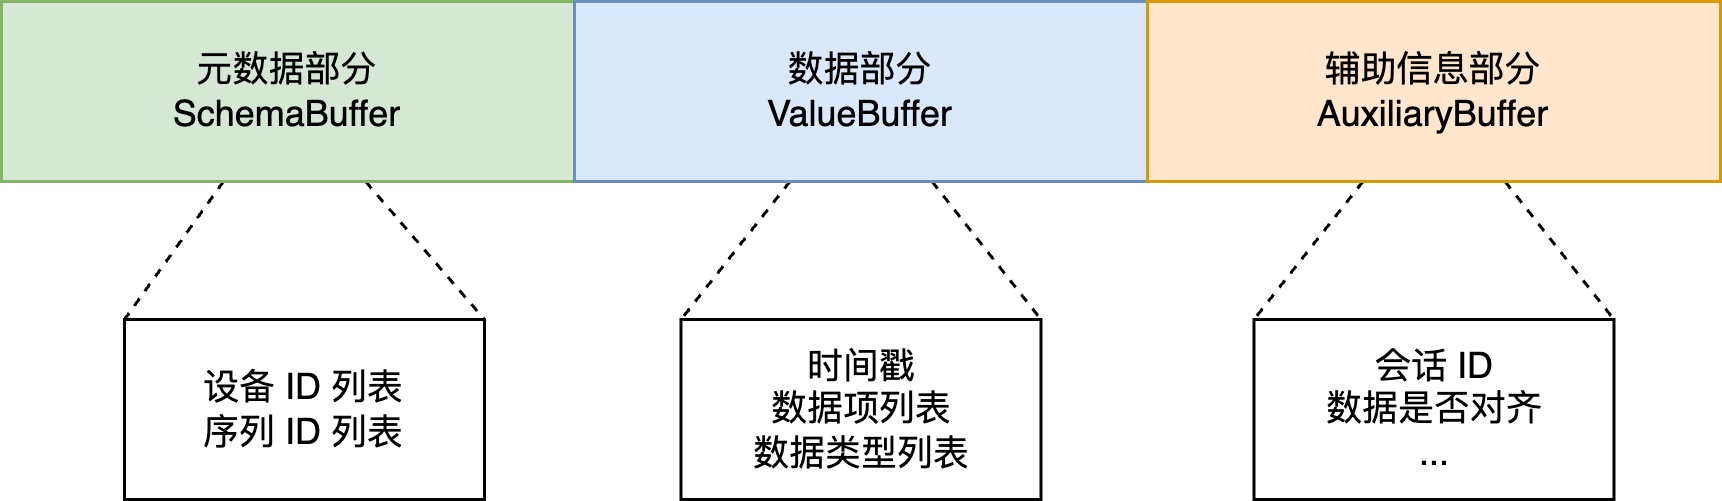
\includegraphics[width=0.9\linewidth]{rpc-general-design.png}
  \caption{写入请求序列化总体设计}
  \label{fig:rpc-general-design}
\end{figure}

在 \ref{sec:chap3-sec2-2-1} 节中,本文介绍了目前 IoTDB 在 Thrift 中对 \emph{insertRecords} 请求的定义。根据各个字段的实际含义,我们可以将它们分成三大部分:元数据部分、数据部分和辅助信息部分。

元数据部分包括设备 ID 和时间序列 ID,它们描述了待写入数据所对应的时间序列都信息。这部分的数据的呈现形式是文本形式,并且其重复度较高,这里的重复度体现在两个方面:
\begin{itemize}
  \item 同一设备或者不同设备的时间序列可能具有相同的 ID,因为它们在现实生活中对应了同样一种类型的实体,例如同样类型的传感器。
  \item 不同设备之间存在部分重复的内容。这是因为 IoTDB 的设备 ID 遵循一种树形的结构,形如 "root.层级1.层级2.层级3"。如果两个设备位于层级树的同一个子树中,那么它们的 ID 中会包含许多相同的部分。
\end{itemize}
针对以上的两个特征,元数据部分非常适合使用字典编码(Dictionary Encoding)进行处理。在本工作的实现中,将元数据部分编码后得到的结果单独保存为一个字节流。

数据部分主要包含时间戳、数值项与数值项的类型。时间戳全都为 8 字节的长整形数据,并且同一个写入请求中不同记录的时间戳可能非常接近;数值项数据可能包含各个类型的数据,如浮点数、整数、字符串等;数据项则都为 1 字节的枚举类型(Enumeration)。数据部分是写入请求序列化后体积最大的部分,对这部分数据进行较为精细化的压缩可以有效减小整个写入请求序列化后的体积。这一部分序列化后的结果也会单独保存为一个字节流。

辅助信息部分主要包括一些标志信息,辅助写入过程中的非核心流程,这部分数据包含会话 ID、数据是否按时间对齐的标志等。这部分数据可能由若干个不同数据类型的标志组成,序列化后的总体积不会很大,因此不需要进行压缩。在未来,\emph{insertRecords} 写入请求中可能会添加更多的辅助信息,因此辅助信息的序列化需要保持一定的拓展性。这一部分序列化后的结果也会单独保存为一个字节流。

下面,本文将分别介绍元数据部分、数据部分和辅助信息部分的序列化设计方案。



\section{写入请求元数据部分序列化与反序列化方案设计}
\subsection{序列化过程}
\begin{figure}
  \centering
  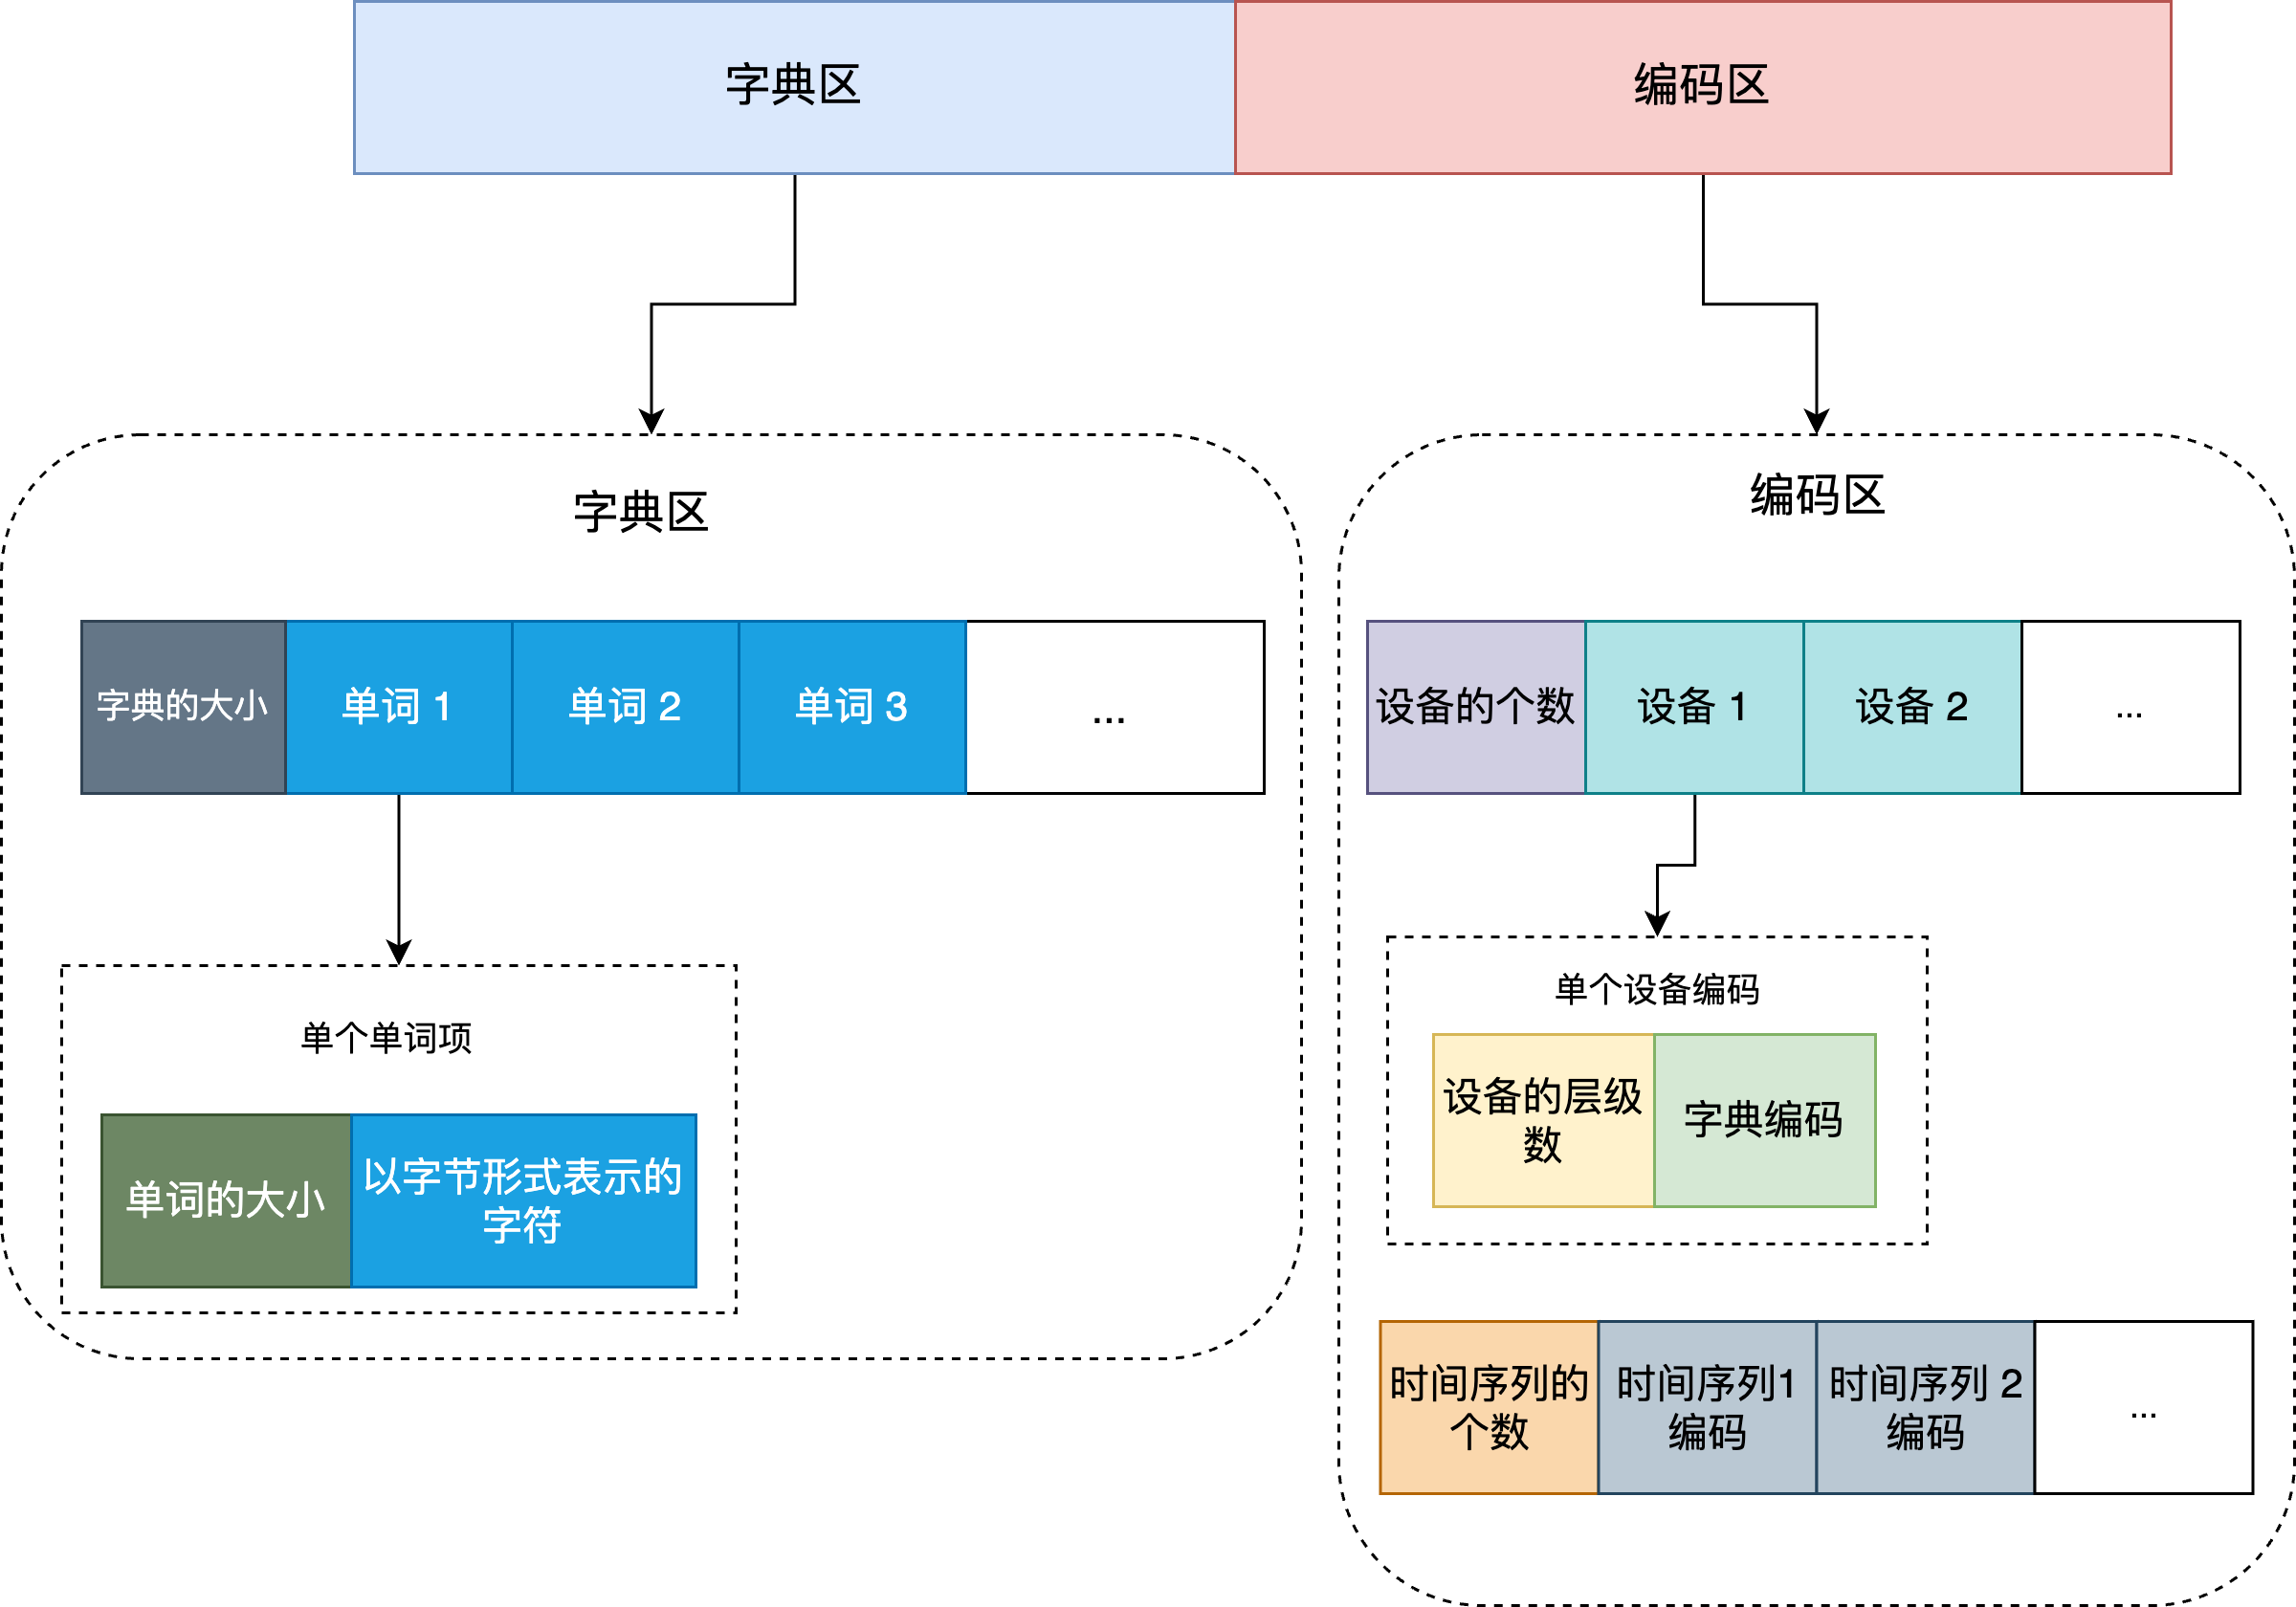
\includegraphics[width=\linewidth]{schema-encoding.png}
  \caption{元数据信息序列化方案设计}
  \label{fig:schema-encoding-general}
\end{figure}

图 \ref{fig:schema-encoding-general} 展示了对 \emph{insertRecords} 写入请求元数据信息序列化方案的总体设计。整体上,元数据信息采用了字典编码的方式进行序列化,字典编码的基本思想是利用一个字典来存储数据中重复出现的元素或模式,并用更短的编码来代替这些重复元素在原数据中的出现,以此来减少数据的体积。如果一个单词出现的频率越高,那么字典编码实现的数据压缩效果就越好。字典编码的核心步骤有两步:构建字典和利用字典进行编码。

 算法 \ref{alg:schema-build-dict} 展示了构建元数据信息序列化字典的过程。在 \emph{insertRecords} 的写入请求中,设备 ID 是一个带有层级结构的字符串,不同层级之间通过字符“.”分隔,形如 "root.层级1.层级2.层级3"。如果我们只是简单地将整个设备 ID 作为一个单词加入到字典中,那么只有当一个设备 ID 重复出现时,才有可能再次利用到这个单词。因为字典编码的压缩效果和单词的出现频率有关,所以为了提高单词的出现频率,本工作将一个设备按照层级拆分成多个单词,然后进行编码。例如 “root.sg.test.d1” 就会被拆分成 root、sg、test、d1 四部分,然后对每一个部分单独进行字典编码,并将编码后的结果拼凑到一起,例如如果 root 对应 1, sg 对应 5,test 对应 3,d1 对应 2,那么编码的结果就是 1532。在这样设计下,即使一个 \emph{insertRecords} 写入请求中的每一个设备 ID 都是不同的,只要这些设备之间存在一些共同的前缀,也都可以通过字典编码进行一定程度的压缩。

与设备 ID 不同,时间序列 ID 则是一个没有层级结构的字符串,不同设备之间可能存在时间序列 ID 相同的序列,因此直接使用整个时间序列 ID 进行编码也可以得到一定的压缩效果。为了更加充分地提高压缩效果,在本工作的设计中,设备 ID 和时间序列 ID 的编码使用共同的字典,因为越大的字典越能挖掘出潜在的编码可能性。

\begin{figure}
  \centering
  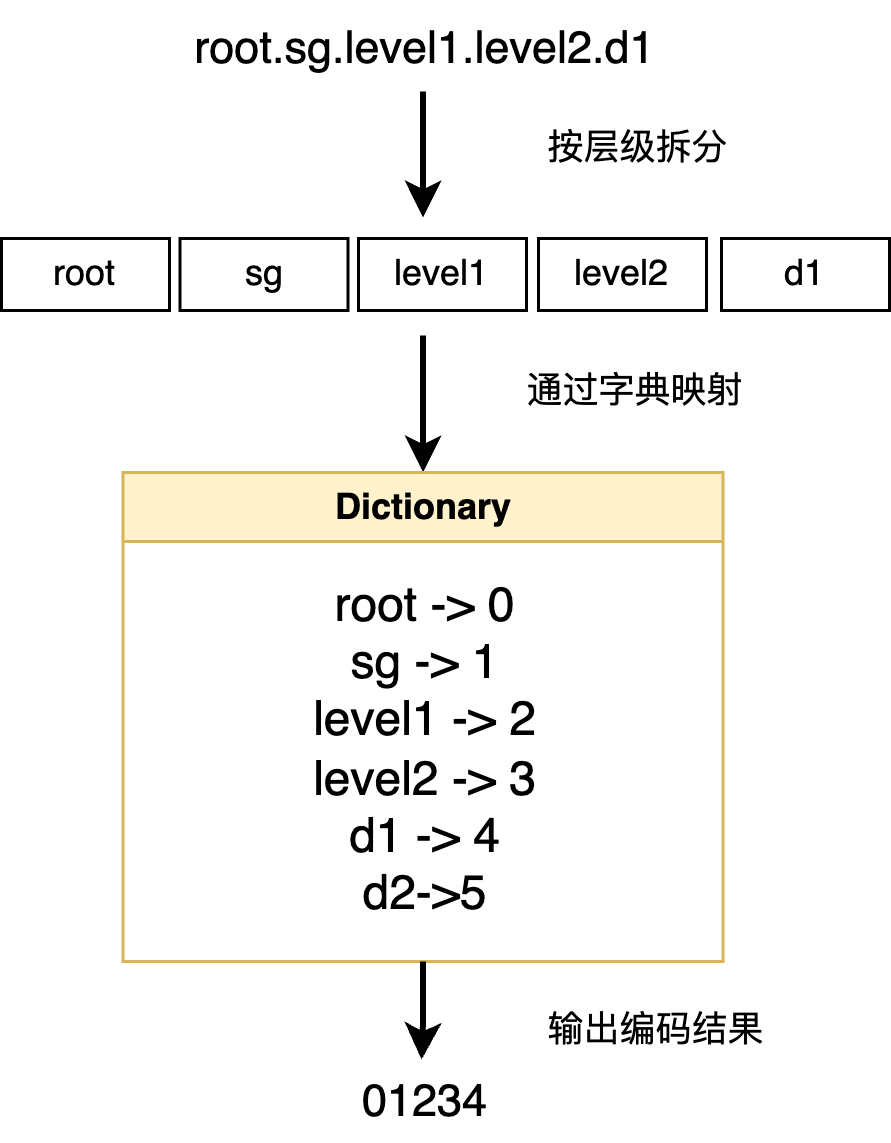
\includegraphics[width=0.55\linewidth]{device-id-encoding-process.png}
  \caption{每一个设备 ID 编码的过程}
  \label{fig:device-id-encoding}
\end{figure}

\begin{algorithm}
  \caption{元数据信息序列化过程构建字典流程}
  \label{alg:schema-build-dict}
  \small
  \begin{algorithmic}
    \REQUIRE \emph{deviceIds} 设备 ID 列表,\emph{timeseriesIDsList} 时间序列 ID 列表

    \STATE 创建一个保序哈希表 \emph{dict}
    \STATE $n\leftarrow$ \emph{deviceIds}.length
    \STATE \emph{counter} $\leftarrow 1$
    \FOR{$i=1$ to $n$}
      \STATE \emph{deviceId} = \emph{deviceIds}.at($i$)
      \STATE 将 \emph{deviceId} 按照 "." 进行切分,得到字符串数组 \emph{words}
      \FOR{\emph{word} in \emph{words}}
        \IF{\emph{word} 不在 \emph{dict} 中}
          \STATE 在 \emph{dict} 中构建映射 \emph{word} $\rightarrow$ \emph{counter}
          \STATE \emph{counter}$++$
        \ENDIF
      \ENDFOR
    \ENDFOR
    \STATE $n \leftarrow$ \emph{timeseriesIDsList}.length
    \FOR{$i=1$ to $n$}
      \STATE \emph{timeseriesIDs} $\leftarrow$ \emph{timeseriesIDsList}.at($i$)
      \STATE $m \leftarrow$ \emph{timeseriesIDs}.length
      \FOR{$j=1$ to $m$}
        \STATE $id \leftarrow$ \emph{timeseriesIDs}.at($j$)
        \IF{\emph{id} 不在 \emph{dict} 中}
          \STATE 在 \emph{dict} 中构建映射 \emph{id} $\rightarrow$ \emph{counter}
          \STATE \emph{counter}$++$
        \ENDIF
      \ENDFOR
    \ENDFOR

    \RETURN \emph{dict}

  \end{algorithmic}
\end{algorithm}

得到字典以后,就需要根据字典对元数据进行编码,主要分为对设备 ID 的编码和时间序列 ID 的编码。对设备的编码比较简单,因为设备 ID 列表是一个单层的列表,所以在编码之前先记录设备 ID 列表的长度。在对每个设备 ID 编码时,先将其按层级拆分,然后记录其层级数,再记录其每个层级所对应的编码值。在对时间序列 ID 进行编码时,因为它是一个两层嵌套的列表,因此不仅要记录外层的长度,也要记录内层每个列表的长度,然后进行查表序列化即可。

前面流程中所得到的字典也需要序列化为字节流,为了便于反序列化,我们将字典所对应的字节流放在了编码结果的前面。在将字典序列化为字节流时需要注意序列化的顺序,因为理论上我们需要记录每个单词所对应的编码值,但是我们为了节省这一部分开销,选择用单词在字典中的位置来代表它所对应的编码值。例如字典中出现的第一个单词就对应编码值 1,第二个单词对应 2,以此类推。算法 \ref{alg:schema-build-encoding} 描述了字典与编码的整个流程。

\begin{algorithm}
  \caption{元数据信息序列化构建编码结果的流程}
  \label{alg:schema-build-encoding}
  \small
  \begin{algorithmic}
    \REQUIRE \emph{deviceIds} 设备 ID 列表,\emph{timeseriesIDsList} 时间序列 ID 列表,\emph{dict} 编码字典

    \STATE 构建一个空字节流 \emph{buffer}
    \STATE 向 \emph{buffer} 中写入 \emph{dict} 的大小
    \FOR{字典中的每一个单词 \emph{word}}
      \STATE 向 \emph{buffer} 中写入 \emph{word} 的长度
      \STATE 向 \emph{buffer} 中写入 \emph{word} 的每一个字母
    \ENDFOR
    
    \STATE 向 \emph{buffer} 中写入 \emph{deviceIds} 的大小
    \FOR{\emph{deviceIds} 中的每一个 \emph{deviceId}}
      \STATE 将 \emph{deviceId} 按照 "." 切分成多个字符串,得到字符串数组 \emph{words}
      \STATE 向 \emph{buffer} 中写入 \emph{words} 的大小
      \FOR{\emph{words} 中的每一个 \emph{word}}
        \STATE 从 \emph{dict} 中查找 \emph{word} 所对应的编码 $e$
        \STATE 将 $e$ 写入到 \emph{buffer} 中
      \ENDFOR
    \ENDFOR

    \STATE 向 \emph{buffer} 中写入 \emph{timeseriesIDsList} 的大小
    \FOR{\emph{timeseriesIDsList} 中的每一个 \emph{timeseriesIDs}}
      \STATE 向 \emph{buffer} 中写入 \emph{timeseriesIDs} 的大小
      \FOR{\emph{timeseriesIDs} 中的每一个 \emph{timeseriesID}}
      \STATE 从 \emph{dict} 中查找 \emph{timeseriesID} 所对应的编码 $e$
      \STATE 向 \emph{buffer} 中写入 $e$
      \ENDFOR
    \ENDFOR

    \RETURN \emph{buffer}


  \end{algorithmic}
\end{algorithm}

\subsection{反序列化过程}
反序列化是序列化的逆过程,算法 \ref{alg:schema-decoding} 描述了元数据信息反序列化的过程。反序列化时先读取字典编码的字典,每个单词所对应的编码值由它在字典中出现的顺序所决定,算法一边读取单词,一边构建一个从编码值到单词的映射表。

将字典反序列化结束以后,就可以逐个读取设备 ID 的和时间序列 ID 的编码值,然后从编码值中恢复这些 ID。因为设备 ID 和时间序列 ID 分别以列表和嵌套列表的形式出现,因此解编码时也要根据字节流中所记录的列表长度信息对列表结构进行还原。


\begin{algorithm}
  \caption{元数据信息反序列化过程}
  \label{alg:schema-decoding}
  \small
  \begin{algorithmic}
    \REQUIRE \emph{buffer} 包含元数据信息的数据字节流
    \STATE 从 \emph{buffer} 中读取字典的大小 $n$
    \STATE 创建哈希表 \emph{dict}
    \FOR{$i=1$ to $n$}
      \STATE 从 \emph{buffer} 读取一个单词的长度 $m$
      \STATE 从 \emph{buffer} 中读取 $m$ 个字符,并构建成一个新的单词 \emph{word}
      \STATE 在 \emph{dict} 中添加映射: $i \rightarrow $ \emph{word}
    \ENDFOR

    \STATE 创建空列表 \emph{deviceIds}
    \STATE 从 \emph{buffer} 中读取设备 ID 的个数 $n$
    \FOR{$i=1$ to $n$}
      \STATE 从 \emph{buffer} 中读取当前设备的层级数 $k$
      \FOR{$j=1$ to $k$}
        \STATE 从 \emph{buffer} 中读取编码值 $e$
        \STATE 从 \emph{dict} 中根据 $e$ 查找到对应的单词
      \ENDFOR
      \STATE 将搜集到的单词拼装起来,使用 "." 连接,并加入到 \emph{deviceIds} 中
    \ENDFOR

    \STATE 创建空列表 \emph{timeseriesIdsList}
    \STATE 从 \emph{buffer} 中读取时间序列列表的个数 $n$
    \FOR{$i=1$ to $n$}
      \STATE 从 \emph{buffer} 中读取当前时间序列列表的长度 $m$
      \STATE 创建一个空列表 \emph{timeseriesIds}
      \FOR{$j=1$ to $m$}
        \STATE 从 \emph{buffer} 中读取编码值 $e$
        \STATE 从 \emph{dict} 中读取对应的单词,并添加到 \emph{timeseriesIds} 中
      \ENDFOR
      \STATE 将 \emph{timeseriesIds} 添加到 \emph{timeseriesIdsList} 中
    \ENDFOR

    \RETURN \emph{deviceIds}, \emph{timeseriesIdsList}

  \end{algorithmic}
\end{algorithm}


\section{数据部分序列化与反序列化方案设计}
\subsection{序列化过程}
对写入请求进行序列化的过程其实本质上是将一份数据转换成字节流,然后传递给下一个处理流程。这个本质与数据存储是类似的,只不过前者将数据交由网络进行传输,而数据存储则将序列化得到的字节流交由磁盘进行存储。因此,我们可以借鉴数据存储领域的一些设计思想。

目前数据库数据存储主要有三种方案:行式存储(Row Storage)、列式存储(Columnar Store)和混合存储(Hybrid Store)。行式存储将一行数据一起保存,相邻的数据项来自不同的列,它们可能类型不同,或者类型相同但是数值的分布不同;列式存储则是将一列数据保存在一起,相邻的数据项不仅类型相同,它们的数值也遵循着共同的分布;混合存储则是将行式存储和列式存储的设计相结合,先将数据按行进行分割成多个块,然后在每个块中按照列的形式存储。行式存储的优势是同一行的数据被聚集在一起,可以方便地访问同一行中的多项数据;列式存储的优势是可以获得更好的压缩比,减少数据体积;混合存储则在一定程度上结合了两者的优势。

同样的,在对写入请求进行序列化时,也可以选择行式存储、列式存储和混合存储。行式存储就是将每一条 Record 的数据一起序列化,列式存储将一条时间序列的数据单独序列化,而混合存储则是先将 Records 分成多批,在每一批内进行列式序列化。

行式序列化的优点在于实现简单,这是因为序列化时一条数据的多个数据项只需要按照顺序逐个转换为字节并添加到字节流中即可,反序列化时也可以按照顺序读取字节流并逐个反序列化单个数据项。但是行式序列化将不同类型的数据全部混合到了一起,导致在压缩时没有办法根据数据的特点进行优化,只能使用通用的压缩算法(如 Snappy\cite{samulowitz2013snappy}、GZip\cite{deutsch1996gzip}、ZSTD\cite{collet2018zstandard} 等)对整体进行压缩,无法实现更加精细化、高效的压缩。

普通的列式序列化将一条时间序列的全部数据都放到一起进行编码,这样数据不仅类型相同,而且都遵循类似的分布,压缩的效果更好。但是,在一个 \emph{insertRecords} 写入请求中,同一条时间序列的数据不会太多,如果只把一条时间序列的若干个数据点放到一起压缩,效果也不好。

为了获取较好的压缩效果,本工作改进了普通列式序列化方案,设计了一种以数据类型为聚集单位的列式序列化方案。图 \ref{fig:value-encoding-general} 展示了数据部分序列化的整体设计,序列化的结果一共分为 3 个区域:时间戳区、数据区和数据类型区。其中,时间戳区只包含时间戳,其中的内容是一个 \emph{insertRecords} 请求中所有记录的时间戳,每个时间戳的大小都固定为 8 字节。数据区包含了具体的数值项,并且这些数值项根据它们的类型被聚集在一起,同一条记录或者不同记录中有相同类型的数据会位于相邻的位置,而同一条记录中类型不同的数据则可能位于较远的位置。除文本类型外,同一数据类型内每个数据项的长度都是相同的。最后一个区域是数据类型区,其包含了写入请求中每个数据项的类型,以及每一行记录的长度。

这样设计的好处在于,我们可以根据每个区域的特点为它们选择合适的压缩算法,而不是只能使用通用的压缩算法进行粗暴的压缩。例如,对于时间戳区,在同一个写入请求中的时间戳通常在数值上都非常接近,因此我们可以选择 Gorilla\cite{pelkonen2015gorilla} 压缩算法对其进行压缩,因为 Gorilla 算法尤其适合用于那些数值波动范围较小的数据;对于 Bool 类型,由于只有 True 和 False 两种取值,我们可以将原本用一个字节表示的数据项变成 1 个 bit,节省了 8 倍的空间。

\begin{figure}
  \centering
  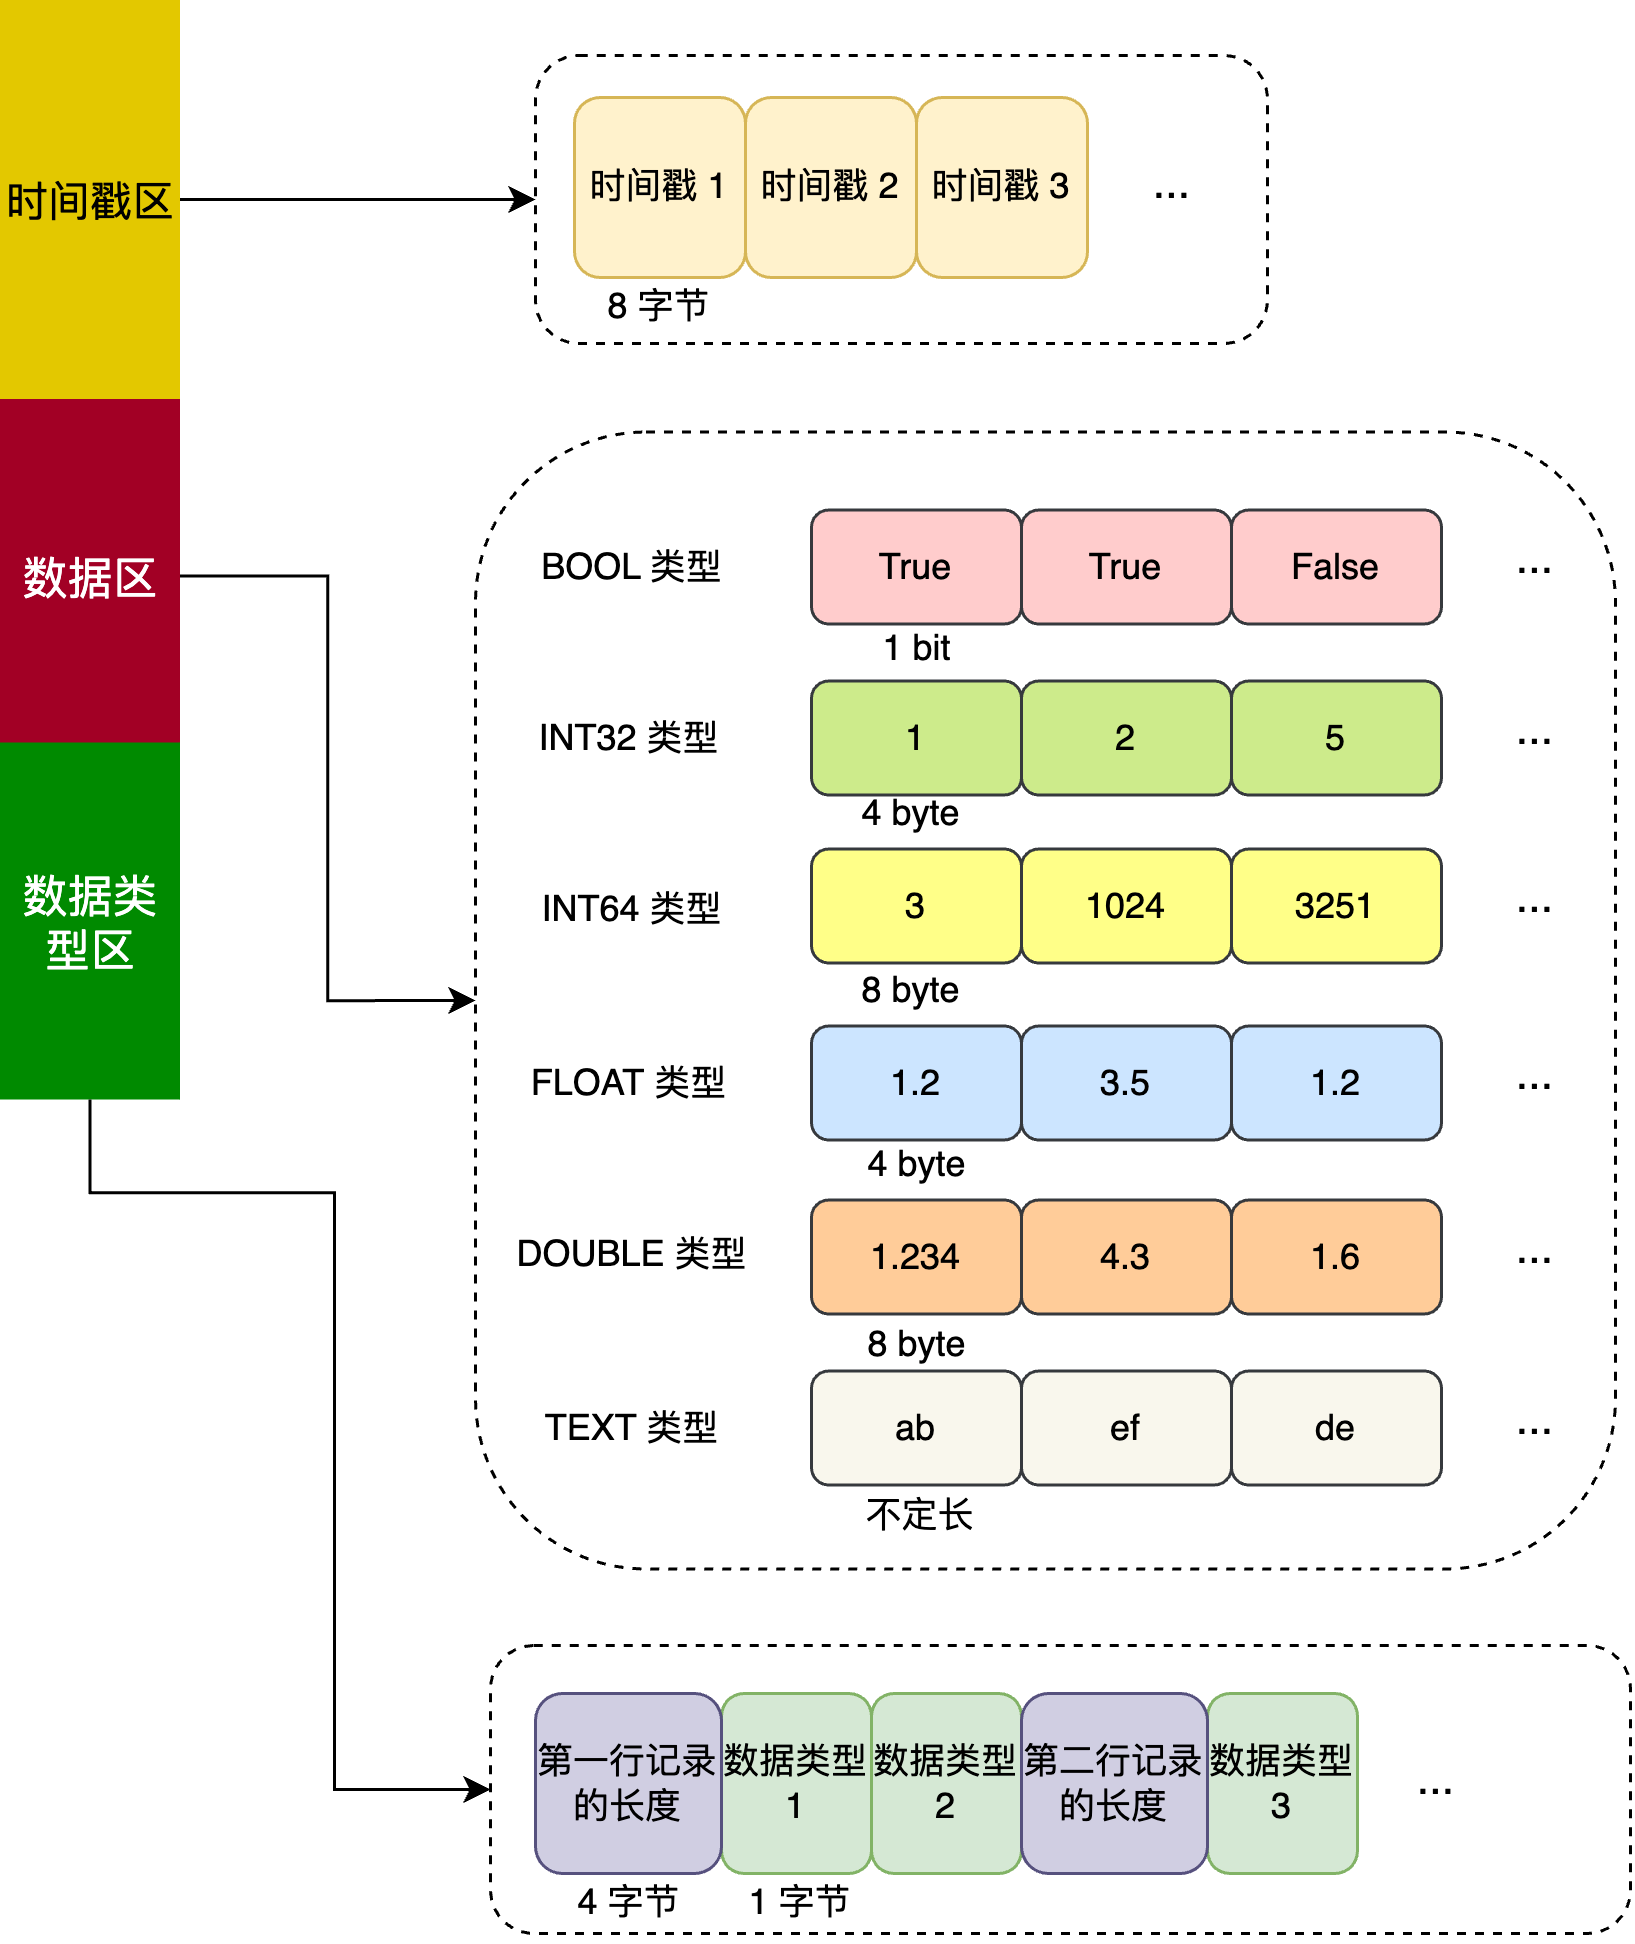
\includegraphics[width= 0.9\linewidth]{value-encoding.png}
  \caption{数据部分序列化设计}
  \label{fig:value-encoding-general}
\end{figure}

算法 \ref{alg:value-encoding} 描述了对写入请求数据部分进行序列化的过程。首先是处理时间戳的部分,将时间戳逐一序列化到一个字节流中,然后使用 Gorilla 压缩算法压缩这个字节流。然后是处理数据的部分,首先将数据按照类型分类,放到多个不同类型的数据列表中,然后将这些数据列表分别进行压缩,最后将压缩后的结果序列化到一个字节流中。在压缩时,我们可以根据数据类型的不同选择合适的压缩算法,如对数值类型选择 Gorilla 算法,这是一种无损的、适用于数据变化幅度不大的压缩算法;对文本类型使用字典压缩算法;对布尔类型使用 Bitpacking 压缩算法\cite{hwang2023lossless}。最后是处理数据类型的部分,将每一行记录的长度和每个数据项的类型序列化到一个字节流中,并最后将这个字节流写入到输出字节流中,数据部分的序列化就完成了。

\begin{algorithm}
  \caption{数据部分序列化过程}
  \label{alg:value-encoding}
  \small
  \begin{algorithmic}
    \REQUIRE \emph{timestamps} 时间戳列表,\emph{datatypesList} 数据类型列表,\emph{valuesList} 数据列表 
    \STATE 创建一个空的字节流 \emph{outputBuffer} 和一个空的字节流 \emph{timeBuffer}
    \STATE 向 \emph{outputBuffer} 中写入 \emph{timestamps} 的大小
    \FOR{\emph{timestamps} 中的每一个 \emph{timestamp}}
      \STATE 将 \emph{timestamp} 写入到 \emph{timeBuffer} 中
    \ENDFOR
    \STATE 对 \emph{timeBuffer} 使用 Gorilla 算法压缩,并将压缩后的结果写入到 \emph{outputBuffer} 中 

    \STATE 创建六个数据列表,分别对应不同的数据类型:\emph{boolList}、\emph{intList}、\emph{longList}、\emph{floatList}、\emph{doubleList}、\emph{textList}
    \STATE 创建一个空的字节流 \emph{typeBuffer}
    \STATE 创建变量 $n = $\emph{datatypesList}.length
    \STATE 将 $n$ 序列化到 \emph{typeBuffer} 中
    \FOR{$i=1$ to $n$}
      \STATE \emph{datatypes} $=$ \emph{datatypesList}.at($i$)
      \STATE 创建变量 $m = $\emph{datatypes}.length
      \STATE 将 $m$ 序列化到 \emph{typeBuffer} 中
      \FOR{$j=1$ to $m$}
        \STATE 根据 \emph{datatypes}.at($j$) 的类型,将 \emph{valuesList}.at($i$).at($j$) 放到对应的数据列表中
        \STATE 将 \emph{datatypes}.at($j$) 的值序列化到 \emph{typeBuffer} 中
      \ENDFOR
    \ENDFOR
    \STATE 将 \emph{boolList} 的大小序列化到 \emph{outputBuffer} 中
    \STATE 将 \emph{boolList} 中的数据按位表示序列化到 \emph{outputBuffer} 中
    \STATE 将 \emph{intList} 的大小序列化到 \emph{outputBuffer} 中
    \STATE 将 \emph{intList} 中的数据使用 Gorilla 压缩后序列化到 \emph{outputBuffer} 中
    \STATE 将 \emph{longList} 的大小序列化到 \emph{outputBuffer} 中
    \STATE 将 \emph{longList} 中的数据使用 Gorilla 压缩后序列化到 \emph{outputBuffer} 中
    \STATE 将 \emph{floatList} 的大小序列化到 \emph{outputBuffer} 中
    \STATE 将 \emph{floatList} 中的数据使用 Gorilla 压缩后序列化到 \emph{outputBuffer} 中
    \STATE 将 \emph{doubleList} 的大小序列化到 \emph{outputBuffer} 中
    \STATE 将 \emph{doubleList} 中的数据使用 Gorilla 压缩后序列化到 \emph{outputBuffer} 中
    \STATE 将 \emph{textList} 的大小序列化到 \emph{outputBuffer} 中
    \STATE 将 \emph{textList} 中的数据使用字典编码后序列化到 \emph{outputBuffer} 中
    \STATE 将 \emph{typeBuffer} 写入到 \emph{outputBuffer} 中
    \RETURN \emph{outputBuffer}

  \end{algorithmic}
\end{algorithm}
\subsection{反序列化过程}
\begin{algorithm}
  \caption{数据部分反序列化过程}
  \label{alg:value-decoding}
  \small
  \begin{algorithmic}
    \REQUIRE \emph{buffer} 包含数据部分的字节流
    \STATE 从 \emph{buffer} 中读取时间戳的个数 $n$
    \STATE 创建一个空的时间戳列表 \emph{timestamps}
    \STATE 创建 Gorilla 解压缩器 \emph{decompressor}
    \FOR{$i=1$ to $n$}
      \STATE 使用 \emph{decompressor} 从 \emph{buffer} 中读取一个时间戳 $t$
      \STATE 将 $t$ 添加到 \emph{timestamps} 中
    \ENDFOR
    \STATE 从 \emph{buffer} 中反序列化出布尔类型的数据列表 \emph{boolList}
    \STATE 从 \emph{buffer} 中反序列化出整数类型的数据列表 \emph{intList}
    \STATE 从 \emph{buffer} 中反序列化出长整数类型的数据列表 \emph{longList}
    \STATE 从 \emph{buffer} 中反序列化出浮点数类型的数据列表 \emph{floatList}
    \STATE 从 \emph{buffer} 中反序列化出双精度浮点数类型的数据列表 \emph{doubleList}
    \STATE 从 \emph{buffer} 中反序列化出文本类型的数据列表 \emph{textList}
    \STATE 从 \emph{buffer} 中读取数据类型列表的个数 $n$
    \STATE 创建一个空的数据类型列表 \emph{datatypesList},一个空的数据列表 \emph{valuesList}
    \FOR{$i=1$ to $n$}
      \STATE 从 \emph{buffer} 中读取当前数据类型列表的长度 $m$
      \STATE 创建一个空的数据类型列表 \emph{datatypes}
      \STATE 创建一个空的数据列表 \emph{values}
      \FOR{$j=1$ to $m$}
        \STATE 从 \emph{buffer} 中读取数据类型 $t$
        \STATE 将 $t$ 添加到 \emph{datatypes} 中
        \STATE 根据 $t$ 从对应的数据列表中读取数据 $v$,并从该数据列表中移除掉该元素
        \STATE 将 $v$ 添加到 \emph{values} 中
    \ENDFOR
    \ENDFOR
    \RETURN \emph{timestamps}, \emph{datatypesList}, \emph{valuesList}
  \end{algorithmic}
\end{algorithm}

算法 \ref{alg:value-decoding} 描述了数据部分反序列化的过程。反序列化时,首先读取时间戳的个数,然后逐一读取时间戳并添加到时间戳列表中。然后从字节流中读取布尔类型、整数类型、长整数类型、浮点数类型、双精度浮点数类型和文本类型的数据列表,并根据对应的压缩算法类型对它们进行解压缩,这些数据列表中的数据是按照序列化时的顺序排列的。最后读取数据类型列表的个数,然后逐一读取每个数据类型列表的长度,再逐一读取每个数据类型列表中的数据类型,每读取一个数据类型,就根据这个数据类型去对应的数据列表中读取最顶部的数据,然后将这个列表顶部的数据移除,并将这个数据添加到一个新的数据列表中。最后返回时间戳列表、数据类型列表和数据列表,反序列化过程就完成了。

\section{写入请求辅助信息部分序列化与反序列化方案设计}

\section{本章小结}
% !TeX root = ../thuthesis-example.tex

\chapter{服务器端高性能 \emph{insertRecords} 写入机制设计与实现}
经过客户端的预处理与 RPC 层的数据传输,写入请求最终会到达服务器端。服务器端对写入请求进行预处理后,交由存储引擎负责处理写入请求,并将这些数据最终持久化到磁盘上,服务器端的设计与实现对写入性能有至关重要的影响。如 \ref{sec:chap3-sec3-1} 中的实验结果所示,现有 IoTDB 服务器端对写入请求的处理有较大的性能瓶颈,不能满足高并发写入请求的需求。因此,本章将介绍对 \emph{insertRecords} 写入请求所设计的服务器端高性能写入机制。


\section{服务器端 \emph{insertRecords} 写入流程总览}
\ref{sec:chap3-sec2} 节介绍了 IoTDB 服务器端对 \emph{insertRecords} 写入请求执行的总体流程,新的执行流程和原有流程大体相似,单针对之前实验中发现的瓶颈,本工作进行了重新设计以优化写入性能。

\begin{figure}
  \centering
  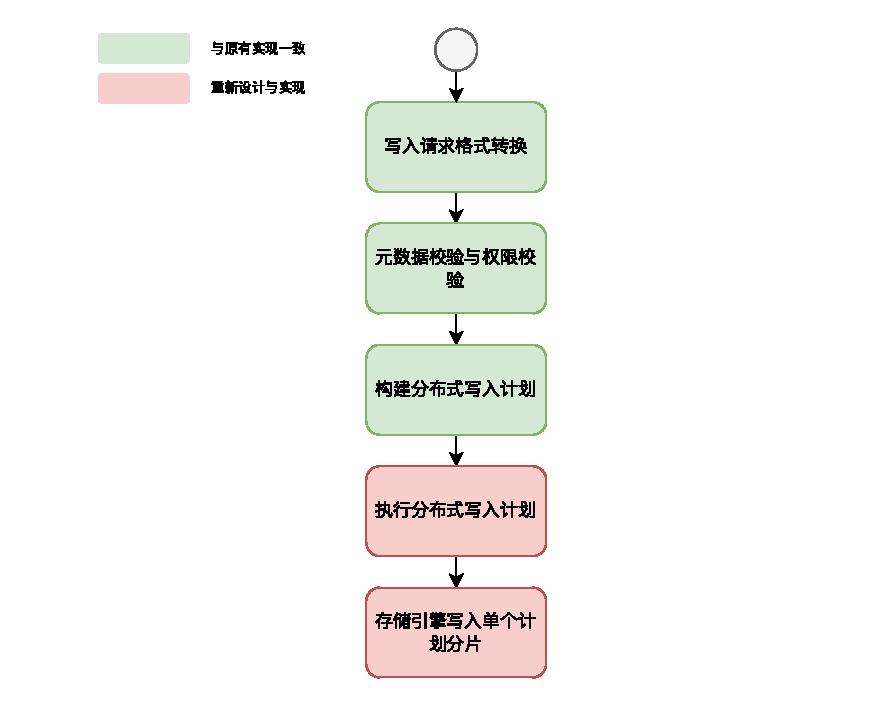
\includegraphics[width=0.9\linewidth]{new-storage-engine.pdf}
  \caption{服务器端 \emph{insertRecords} 写入流程}
  \label{fig:iotdb-insertRecords-flow}
\end{figure}

图 \ref{fig:iotdb-insertRecords-flow} 展示了 \emph{insertRecords} 写入请求到达 IoTDB 服务器端以后的总体执行流程,其中绿色部分代表这些流程与 IoTDB 原有设计基本保持一致,因为它们并不是写入的瓶颈所在;红色部分代表了在原有实现中存在的性能瓶颈,本工作对这些部分进行了重新设计与实现以提高写入性能。


在执行分布式写入计划时,一个写入请求会被分为多个写入计划分片(称为 FragmentInstance,FI),每个分片都是写入到一个 DataRegion 中的计划。根据 DataRegion 的分布,可以将其分为本地 DataRegion 和远程 DataRegion,本地 DataRegion 是指存储引擎所在的节点上的 DataRegion,远程 DataRegion 是指存储引擎所在节点以外的 DataRegion。为了充分利用多核 CPU 的计算能力,本工作将写入本地和写入远程 DataRegion 的过程都设计为了多线程并行执行,以提高写入性能。

在存储引擎写入单个计划分片时,不仅需要将数据记录到内存表中,还需要执行记录写前日志、更新监控信息、维护内存索引等操作。这些操作大部分都不是核心的写入操作,但是却会对写入性能产生较大的影响。因此,本工作通过批量化的形式,将这些操作的代价分摊到多行写入记录上,以减少这些操作对写入性能的影响。例如,原本每写入一行记录就需要记录一次写前日志、更新一次监控信息、维护一次内存索引,现在可以将这些操作批量化,每写入一批记录才执行一次这些操作,这样平均到每一条记录上的代价就大大减小了。最后,为了改善前文提到的使用 \emph{insertRecords} 接口进行写入时写前日志过多的问题,本工作对写前日志进行了压缩,减少了写前日志对磁盘的写入量,提高了写入性能。下面将详细介绍这些优化措施的设计与实现。

\section{多线程并行写入设计与实现}
\subsection{多线程并行写入设计}
图 \ref{fig:fi-parallel-write} 展示了 FragmentInstance 多线程并行写入的总体架构。多线程并行写入的设计分为写入本地 DataRegion 和写入远程 DataRegion 两部分,下面将分别介绍这两部分的设计。

\begin{figure}
  \centering
  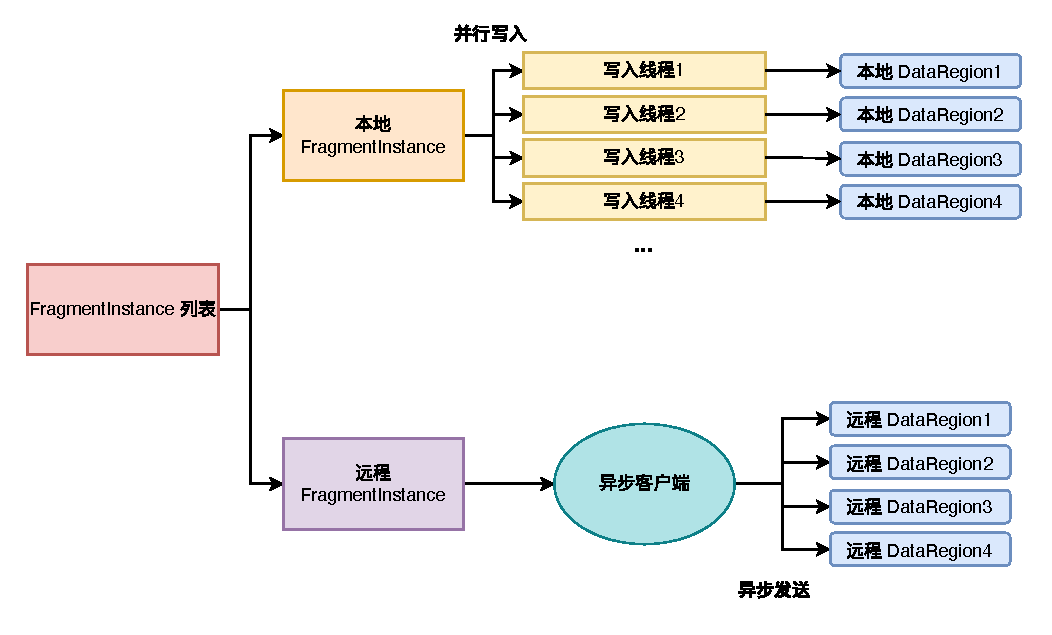
\includegraphics[width=\linewidth]{FragmentInstance写入.pdf}
  \caption{多线程并行写入设计}
  \label{fig:fi-parallel-write}
\end{figure}

在一般的系统中,对一项任务的并行执行通常会构建一个线程池负责此工作,以减少线程创建与销毁的开销,在本工作的设计中遵循了这一种范式。因此,想要实现多线程并行写入,我们首先要确定线程池的大小。如果线程池中的线程数过少,那么无法充分利用多核 CPU 的计算能力,从而无法提高写入性能;如果线程池中的线程数过多,那么会增加线程创建与销毁的开销,反而会降低写入性能。根据线程数与 DataRegion 的个数的比例,可以分为多个线程写一个 DataRegion、一个线程写一个 DataRegion 和一个线程写多个 DataRegion 三种情况。在目前 IoTDB 的设计与实现中,每个 DataRegion 都有一个锁,用于保证对 DataRegion 的读写操作是线程安全的。此外,一个 DataRegion 也对应了一个共识组,共识层为了保证数据的一致性,也持有一个锁。在这样的设计下,针对一个 DataRegion 的写入是串行的,即一次只能有一个线程写入一个 DataRegion。

综合以上因素,本工作选择了一个线程写一个本地 DataRegion 的设计,即每个 DataRegion 都有一个专门的线程负责处理这个 DataRegion 的写入任务。为了处理多个写入请求,每个 DataRegion 的线程都会维护一个写入队列,用于存放待写入的数据。不同写入请求对同一个 DataRegion 的写入任务会被放入同一个队列中,该 DataRegion 对应的写入线程会不断从写入队列中取出任务进行处理。为了避免过多任务堆积,任务队列的大小是有限的,超过了队列的大小后,新的写入请求会被拒绝,并向客户端返回写入失败的信息。写入请求向写入队列提交写入任务后,会获得一个 Future 对象,用于知晓写入任务的执行结果。写入任务执行完成后,Future 对象会被设置为完成状态,并且可以通过 Future 对象获取写入任务的执行结果。

对远程 DataRegion 的写入通过网络发送,在系统内缓存了一个全局的客户端池,它们负责将对远程 DataRegion 写入的 FragmentInstance 异步地发送到对应的节点上,并且返回一个 Future 对象,用于后续的处理。

当写入本地 DataRegion 和远程 DataRegion 的 FragmentInstance 都被异步地分发之后,主写入线程会拿到所有这些 FragmentInstance 对应的 Future 对象,并通过这些对象等待它们全部完成,随后将写入结果返回给客户端。

\subsection{多线程并行写入实现}
为了实现上述的设计,本工作通过一个 FragmentInsertPoolManager 类来管理每个本地 DataRegion 的写入,该类的字段和方法如表 \ref{tabular:fragment-insertion-pool-manager-fields} 和表 \ref{tabular:fragment-insertion-pool-manager-methods} 所示。

\begin{table}
  \centering
  \caption{FragmentInsertPoolManager 类字段}
  \label{tabular:fragment-insertion-pool-manager-fields}
  \begin{tabular}{lp{5cm}p{5cm}}
    \toprule
    字段名 & 字段类型 & 字段描述 \\
    \midrule
    instance & FragmentInsertPoolManager & 单例模式 \\
    executionPoolMap & Map<ConsensusGroupId, ExecutorService> & 记录每个 DataRegion 对应的线程池 \\
    \bottomrule
  \end{tabular}
\end{table}

\begin{table}
  \centering
  \caption{FragmentInsertPoolManager 类方法}
  \label{tabular:fragment-insertion-pool-manager-methods}
  \begin{tabular}{lp{5cm}p{5cm}}
    \toprule
    方法名 & 方法参数 & 方法描述 \\
    \midrule
    getInstance & 无 & 获取 FragmentInsertPoolManager 的单例 \\
    registerPool & 一个 DataRegion 以及一个 ExecutorService & 注册这个 DataRegion 对应的写入线程,便于后续的写入任务分发 \\
    submitTask & ConsensusGroupId 以及写入任务 & 将写入任务提交到对应的 DataRegion 的写入线程池中执行 \\
    \bottomrule
  \end{tabular}
\end{table}

FragmentInsertPoolManager 的核心方法是 registerPool 和 submitTask。当一个 DataRegion 被创建或者恢复时,它会创建一个单线程的线程池,用于执行所有写入到本 DataRegion 的 FragmentInstance,然后调用 FragmentInsertPoolManager 的 registerPool 方法,将这个线程池注册到 FragmentInsertPoolManager 中。当执行写入请求的主线程开始执行分布式写入计划时,它会调用 FragmentInsertPoolManager 的 submitTask 方法,将写入任务提交到对应的 DataRegion 的写入线程池中执行。

对于远程的 DataRegion 写入,本工作通过网络的异步发送来完成并行写入。在 IoTDB 中,每个 DataNode 都为与其他 DataNode 的连接维护了一个全局的客户端池。当需要写入远程 DataRegion 时,主写入线程会从客户端池中获取一个客户端,然后将写入任务通过客户端的异步发送接口发送到对应的 DataNode 上。异步发送接口由 Thrift 实现,这个接口要求上层传入一个回调函数,当发送完成后会调用这个回调函数。主写入线程通过这个回调函数来知晓写入任务的执行结果。

由于网络传输的原因,写入远端 DataRegion 的耗时会更久。为了更高效地执行写入,主写入线程会先发送对远端 DataRegion 的写入请求,然后再将对本地 DataRegion 的写入请求提交到线程池中执行,此时远端和本地的写入都在并行执行。等到所有的写入请求都执行完成后,主写入线程再将写入结果返回给客户端。

\section{批量化写入设计与实现}
\subsection{批量化写入设计}
批量化写入一共分为三点:批量化写前日志、批量化更新监控信息和批量化维护内存索引。在 IoTDB 的设计中,每次写入一行数据都会记录一次写前日志、更新一次监控信息和维护一次内存索引,这些操作都会对写入性能产生较大的影响。因此,本工作将这些操作批量化,每次写入一批数据才执行一次这些操作,以减少这些操作对写入性能的影响。

\subsubsection{批量化写前日志}
\begin{figure}
  \centering
  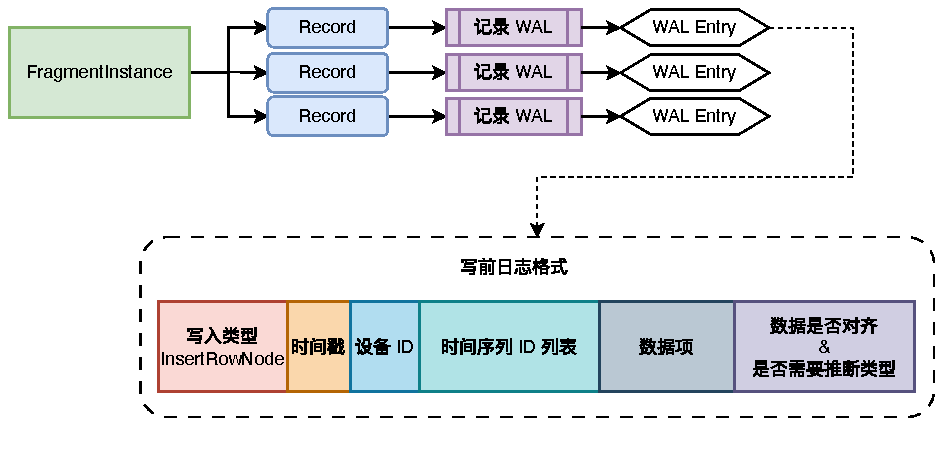
\includegraphics[width=\linewidth]{origin-wal-format.pdf}
  \caption{原有写入日志格式}
  \label{fig:origin-wal-format}
\end{figure}

图 \ref{fig:origin-wal-format} 展示了在原有 IoTDB 的实现中,一个 FragmentInstance 在写入时记录写前日志的流程和格式。对一个 FragmentInstance 中的每一行记录,都需要单独记录一次写前日志,每次都需要重复记录这些记录的时间戳、设备 ID、时间序列 ID 和数值项等,而这其中有相当一部分信息是重复的。这样的设计会导致写前日志的体积过大,对磁盘的写入量也会增加,从而影响写入性能。

// TODO:判断是否要写写前日志批量化的工作
\subsubsection{批量化更新监控信息}
 IoTDB 的监控系统负责监控 IoTDB 运行时的各类指标,以便于用户和开发者了解 IoTDB 的状态,并进行运维和调优。
 在 IoTDB 现有的实现中,每写入一个 FragmentInstance 中的一行记录,就需要更新对应的监控信息,包括创建内存表的耗时、写入写前日志的耗时、写入内存表的耗时、更新内存缓存的耗时等。监控系统为这些监控项都维护了对应的直方图,因此每次写入一行记录需要更多这些监控项对应的直方图。从 \ref{sec:chap3-sec3-1} 节中对 \emph{insertRecords} 和 \emph{insertTablets} 的实验中可以看出,\emph{insertRecords} 写入时更新监控信息的开销明显较大。因此,本工作将这些监控信息的更新批量化,每次写入一批数据才更新一次这些监控信息,以减少这些操作对写入性能的影响。

 为了实现这一点,我们修改了更新监控信息的时机和逻辑。每行记录在写入时,仍会记录各个阶段的耗时,但不会将这些耗时立马更新到监控系统里,而是将这些耗时记录在一个本地的数据结构中。这个数据结构只记录这一个写入请求的监控指标,当这个写入请求的每一个 FragmentInstance 都写完了以后,再统一将这些监控指标更新到监控系统中。在这样的设计下,原本执行一次 \emph{insertRecords} 更新监控框架的次数为写入数据的行数,现在则变成了一次,这样就大大减少了更新监控信息对写入性能的影响。

\subsubsection{批量化维护内存缓存}
IoTDB 支持一种名为 Last 查询的查询方式,它可以查询某个时间序列写入数据库的最后一个数据点。为了提高 Last 查询的性能,IoTDB 在内存中维护了一个名为 LastCache 的缓存,其中保存了每个时间序列写入数据库的最后一个数据点。在每次写入时,都需要对这个缓存进行维护。在 IoTDB 的现有实现中,每次写入一行记录都要维护一次这个缓存,这样会导致写入性能下降,从表 \ref{tabular:insert-records-profile-result} 中可以看出,维护内存缓存在 \emph{insertRecords} 写入的性能开销中占有较大的比例。

为了减少维护内存缓存对写入性能的影响,本工作将维护内存缓存的操作批量化,每次写入一个 FragmentInstance 之后才批量化地更新一次缓存。并且,更新缓存之前,先对 FragmentInstance 中的数据进行排序和去重,只更新写入的时间序列的最后一个点。之所以这样设计,是因为 LastCache 的设计比较复杂,反复更新 LastCache 的代价较大,因此我们选择提前处理好数据,以尽可能地减少对 LastCache 的更新。
\subsubsection{批量化写入内存表}
在如今的 \emph{insertRecords} 实现中,写入内存表的操作是行式的,即数据是一行一行地写入到内存表中的。这样的效率并不高,因为每写入一行都要调用许多辅助函数,函数调用的开销无法均摊。此外,这样的写入方式对 CPU 的缓存也并不友好\cite{boncz2005monetdb}。为了提高写入内存表时的效率,本工作将这个过程批量化,在写入之前先对数据进行排序和归类,将写入到同一个内存表的数据聚集到一起,然后一次性地写入到内存表中,以减少函数调用的开销和提高 CPU 缓存的命中率。

\subsection{批量化写入实现}
本工作对上述批量化执行设计进行了实现。

\section{写前日志压缩设计与实现}
\subsection{写前日志压缩设计}
\subsection{写前日志压缩实现}
% !TeX root = ../thuthesis-example.tex

\chapter{服务器端高性能写入机制设计与实现}
经过客户端的预处理与 RPC 层的数据传输,写入请求最终会到达服务器端。服务器端对写入请求进行预处理后,交由存储引擎负责处理写入请求,并将这些数据最终持久化到磁盘上,服务器端的设计与实现对写入性能有至关重要的影响。如 \ref{sec:chap3-sec3-1} 中的实验结果所示,现有 IoTDB 服务器端对写入请求的处理有较大的性能瓶颈,不能满足高并发写入请求的需求。因此,本章将介绍对 \emph{insertRecords} 写入请求所设计的服务器端高性能写入机制。


\section{服务器端 \emph{insertRecords} 写入流程总览}
\ref{sec:chap3-sec2} 节介绍了 IoTDB 服务器端对 \emph{insertRecords} 写入请求执行的总体流程,新的执行流程和原有流程大体相似,但针对之前实验中发现的瓶颈,本工作进行了重新设计以优化写入性能。

\begin{figure}
  \centering
  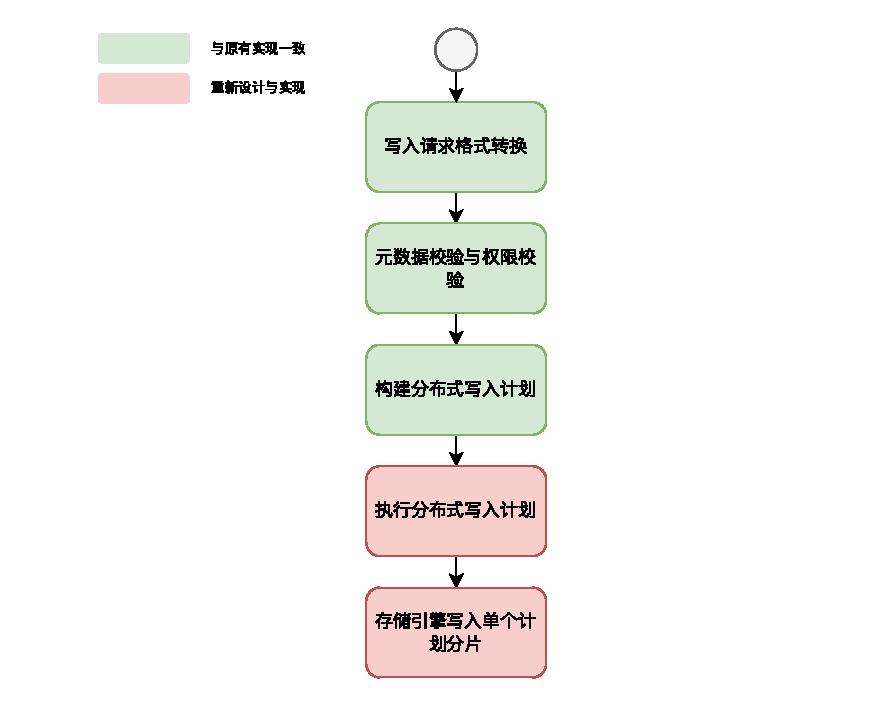
\includegraphics[width=0.9\linewidth]{new-storage-engine.pdf}
  \caption{服务器端 \emph{insertRecords} 写入流程}
  \label{fig:iotdb-insertRecords-flow}
\end{figure}

图 \ref{fig:iotdb-insertRecords-flow} 展示了 \emph{insertRecords} 写入请求到达 IoTDB 服务器端以后的总体执行流程,其中绿色部分代表这些流程与 IoTDB 原有设计基本保持一致,因为它们并不是写入的瓶颈所在;红色部分代表了在原有实现中存在的性能瓶颈,本工作对这些部分进行了重新设计与实现以提高写入性能。


在执行分布式写入计划时,一个写入请求会被分为多个写入计划分片(称为 FragmentInstance,FI),每个分片都是写入到一个 DataRegion 中的计划。根据 DataRegion 的分布,可以将其分为本地 DataRegion 和远程 DataRegion,本地 DataRegion 是指存储引擎所在的节点上的 DataRegion,远程 DataRegion 是指存储引擎所在节点以外的 DataRegion。为了充分利用多核 CPU 的计算能力,本工作将写入本地和写入远程 DataRegion 的过程都设计为了多线程并行执行,以提高写入性能。

在存储引擎写入单个计划分片时,不仅需要将数据记录到内存表中,还需要执行记录写前日志、更新监控信息、维护内存索引等操作。这些操作大部分都不是核心的写入操作,但是却会对写入性能产生较大的影响。因此,本工作通过批量化的形式,将这些操作的代价分摊到多行写入记录上,以减少这些操作对写入性能的影响。例如,原本每写入一行记录就需要记录一次写前日志、更新一次监控信息、维护一次内存索引,现在可以将这些操作批量化,每写入一批记录才执行一次这些操作,这样平均到每一条记录上的代价就大大减小了。最后,为了改善前文提到的使用 \emph{insertRecords} 接口进行写入时写前日志过多的问题,本工作对写前日志进行了压缩,减少了写前日志对磁盘的写入量,提高了写入性能。下面将详细介绍这些优化措施的设计与实现。

\section{多线程并行写入设计与实现}
\subsection{多线程并行写入设计}
图 \ref{fig:fi-parallel-write} 展示了 FragmentInstance 多线程并行写入的总体架构。多线程并行写入的设计分为写入本地 DataRegion 和写入远程 DataRegion 两部分,下面将分别介绍这两部分的设计。

\begin{figure}
  \centering
  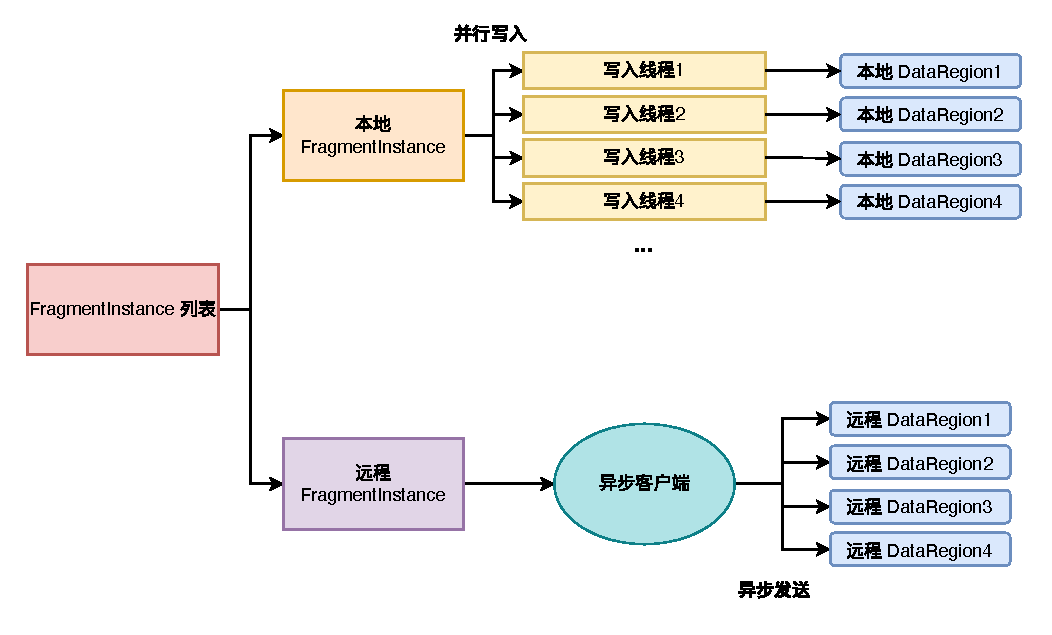
\includegraphics[width=\linewidth]{FragmentInstance写入.pdf}
  \caption{多线程并行写入设计}
  \label{fig:fi-parallel-write}
\end{figure}

在一般的系统中,对一项任务的并行执行通常会构建一个线程池负责此工作,以减少线程创建与销毁的开销,在本工作的设计中遵循了这一种范式。因此,想要实现多线程并行写入,我们首先要确定线程池的大小。如果线程池中的线程数过少,那么无法充分利用多核 CPU 的计算能力,从而无法提高写入性能;如果线程池中的线程数过多,那么会增加线程创建与销毁的开销,反而会降低写入性能。根据线程数与 DataRegion 的个数的比例,可以分为多个线程写一个 DataRegion、一个线程写一个 DataRegion 和一个线程写多个 DataRegion 三种情况。在目前 IoTDB 的设计与实现中,每个 DataRegion 都有一个锁,用于保证对 DataRegion 的读写操作是线程安全的。此外,一个 DataRegion 也对应了一个共识组,共识层为了保证数据的一致性,也持有一个锁。在这样的设计下,针对一个 DataRegion 的写入是串行的,即一次只能有一个线程写入一个 DataRegion。

综合以上因素,本工作选择了一个线程写一个本地 DataRegion 的设计,即每个 DataRegion 都有一个专门的线程负责处理这个 DataRegion 的写入任务。为了处理多个写入请求,每个 DataRegion 的线程都会维护一个写入队列,用于存放待写入的数据。不同写入请求对同一个 DataRegion 的写入任务会被放入同一个队列中,该 DataRegion 对应的写入线程会不断从写入队列中取出任务进行处理。为了避免过多任务堆积,任务队列的大小是有限的,超过了队列的大小后,新的写入请求会被拒绝,并向客户端返回写入失败的信息。写入请求向写入队列提交写入任务后,会获得一个 Future 对象,用于知晓写入任务的执行结果。写入任务执行完成后,Future 对象会被设置为完成状态,并且可以通过 Future 对象获取写入任务的执行结果。

对远程 DataRegion 的写入通过网络发送,在系统内缓存了一个全局的客户端池,它们负责将对远程 DataRegion 写入的 FragmentInstance 异步地发送到对应的节点上,并且返回一个 Future 对象,用于后续的处理。

当写入本地 DataRegion 和远程 DataRegion 的 FragmentInstance 都被异步地分发之后,主写入线程会拿到所有这些 FragmentInstance 对应的 Future 对象,并通过这些对象等待它们全部完成,随后将写入结果返回给客户端。

\subsection{多线程并行写入实现}
为了实现上述的设计,本工作通过一个 FragmentInsertPoolManager 类来管理每个本地 DataRegion 的写入,该类的字段和方法如表 \ref{tabular:fragment-insertion-pool-manager-fields} 和表 \ref{tabular:fragment-insertion-pool-manager-methods} 所示。

\begin{table}
  \centering
  \caption{FragmentInsertPoolManager 类字段}
  \label{tabular:fragment-insertion-pool-manager-fields}
  \begin{tabular}{lp{5cm}p{5cm}}
    \toprule
    字段名 & 字段类型 & 字段描述 \\
    \midrule
    instance & FragmentInsertPoolManager & 单例模式 \\
    executionPoolMap & Map<ConsensusGroupId, ExecutorService> & 记录每个 DataRegion 对应的线程池 \\
    \bottomrule
  \end{tabular}
\end{table}

\begin{table}
  \centering
  \caption{FragmentInsertPoolManager 类方法}
  \label{tabular:fragment-insertion-pool-manager-methods}
  \begin{tabular}{lp{5cm}p{5cm}}
    \toprule
    方法名 & 方法参数 & 方法描述 \\
    \midrule
    getInstance & 无 & 获取 FragmentInsertPoolManager 的单例 \\
    registerPool & 一个 DataRegion 以及一个 ExecutorService & 注册这个 DataRegion 对应的写入线程,便于后续的写入任务分发 \\
    submitTask & ConsensusGroupId 以及写入任务 & 将写入任务提交到对应的 DataRegion 的写入线程池中执行 \\
    \bottomrule
  \end{tabular}
\end{table}

FragmentInsertPoolManager 的核心方法是 registerPool 和 submitTask。当一个 DataRegion 被创建或者恢复时,它会创建一个单线程的线程池,用于执行所有写入到本 DataRegion 的 FragmentInstance,然后调用 FragmentInsertPoolManager 的 registerPool 方法,将这个线程池注册到 FragmentInsertPoolManager 中。当执行写入请求的主线程开始执行分布式写入计划时,它会调用 FragmentInsertPoolManager 的 submitTask 方法,将写入任务提交到对应的 DataRegion 的写入线程池中执行。

对于远程的 DataRegion 写入,本工作通过网络的异步发送来完成并行写入。在 IoTDB 中,每个 DataNode 都为与其他 DataNode 的连接维护了一个全局的客户端池。当需要写入远程 DataRegion 时,主写入线程会从客户端池中获取一个客户端,然后将写入任务通过客户端的异步发送接口发送到对应的 DataNode 上。异步发送接口由 Thrift 实现,这个接口要求上层传入一个回调函数,当发送完成后会调用这个回调函数。主写入线程通过这个回调函数来知晓写入任务的执行结果。

由于网络传输的原因,写入远端 DataRegion 的耗时会更久。为了更高效地执行写入,主写入线程会先发送对远端 DataRegion 的写入请求,然后再将对本地 DataRegion 的写入请求提交到线程池中执行,此时远端和本地的写入都在并行执行。等到所有的写入请求都执行完成后,主写入线程再将写入结果返回给客户端。

\section{批量化写入设计与实现}
\subsection{批量化写入设计}
批量化写入一共分为三点:批量化写前日志、批量化更新监控信息和批量化维护内存索引。在 IoTDB 的设计中,每次写入一行数据都会记录一次写前日志、更新一次监控信息和维护一次内存索引,这些操作都会对写入性能产生较大的影响。因此,本工作将这些操作批量化,每次写入一批数据才执行一次这些操作,以减少这些操作对写入性能的影响。

\subsubsection{批量化写前日志}
\begin{figure}
  \centering
  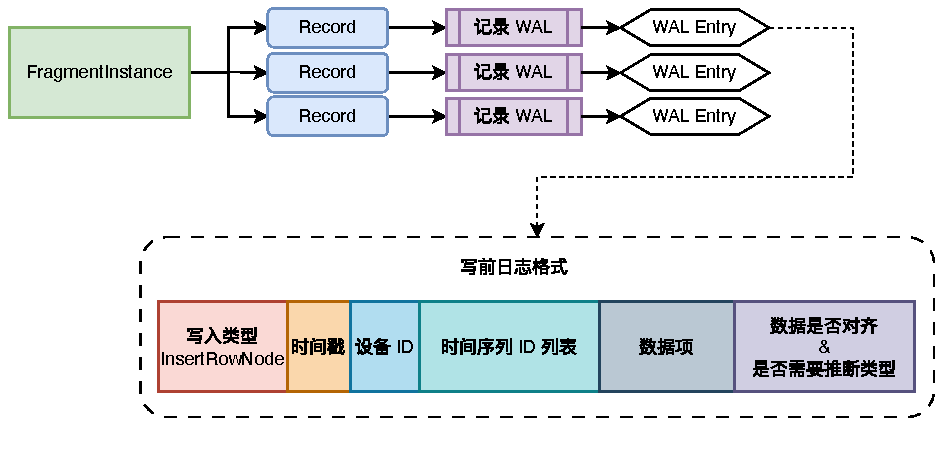
\includegraphics[width=\linewidth]{origin-wal-format.pdf}
  \caption{原有写入日志格式}
  \label{fig:origin-wal-format}
\end{figure}

图 \ref{fig:origin-wal-format} 展示了在原有 IoTDB 的实现中,一个 FragmentInstance 在写入时记录写前日志的流程和格式。对一个 FragmentInstance 中的每一行记录,都需要单独记录一次写前日志,每次都需要重复记录这些记录的时间戳、设备 ID、时间序列 ID 和数值项等,而这其中有相当一部分信息是重复的。这样的设计会导致写前日志的体积过大,对磁盘的写入量也会增加,从而影响写入性能。

\begin{figure}
  \centering
  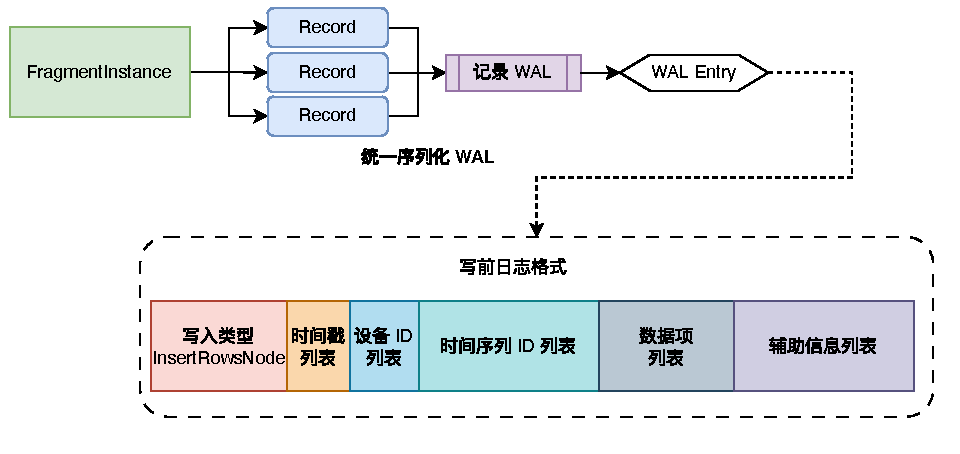
\includegraphics[width=\linewidth]{批量化wal设计.pdf}
  \caption{批量化 WAL 序列化设计}
  \label{fig:batch-wal-design}
\end{figure}

 如果要减小写前日志的体积,我们可以参考第 \ref{sec:chap6} 章的设计,将一个 FragmentInstance 中的所有记录集中在一起序列化,并使用字典压缩、Gorilla 编码等方法针对设备 ID、测点 ID、时间戳等各部分进行针对性的压缩。但是这样会显著增加写入时的 CPU 开销,让每次写入的延迟变高,反而有可能降低写入性能。因此,我们决定结合 \ref{sec:chap7-sec4} 节的工作,先将一个 FragmentInstance 中的所有记录集合在一起,然后将它们的设备 ID、时间序列 ID、时间戳等信息统一序列化到写前日志中,图 \ref{fig:batch-wal-design} 展示了将一个 FragmentInstance 中所有记录一起记录写前日志的设计。这样虽然不能减少写前日志的体积,但是可以将具有相似性的数据聚集到一起,提高数据的局部性。而压缩算法通常利用数据的冗余信息来进行压缩,提高数据的局部性可以使得后续对数据进行压缩时的效率变得更高。
\subsubsection{批量化更新监控信息}
 IoTDB 的监控系统负责监控 IoTDB 运行时的各类指标,以便于用户和开发者了解 IoTDB 的状态,并进行运维和调优。
 在 IoTDB 现有的实现中,每写入一个 FragmentInstance 中的一行记录,就需要更新对应的监控信息,包括创建内存表的耗时、写入写前日志的耗时、写入内存表的耗时、更新内存缓存的耗时等。监控系统为这些监控项都维护了对应的直方图,因此每次写入一行记录需要更多这些监控项对应的直方图。从 \ref{sec:chap3-sec3-1} 节中对 \emph{insertRecords} 和 \emph{insertTablets} 的实验中可以看出,\emph{insertRecords} 写入时更新监控信息的开销明显较大。因此,本工作将这些监控信息的更新批量化,每次写入一批数据才更新一次这些监控信息,以减少这些操作对写入性能的影响。

 为了实现这一点,我们修改了更新监控信息的时机和逻辑。每行记录在写入时,仍会记录各个阶段的耗时,但不会将这些耗时立马更新到监控系统里,而是将这些耗时记录在一个本地的数据结构中。这个数据结构只记录这一个写入请求的监控指标,当这个写入请求的每一个 FragmentInstance 都写完了以后,再统一将这些监控指标更新到监控系统中。在这样的设计下,原本执行一次 \emph{insertRecords} 更新监控框架的次数为写入数据的行数,现在则变成了一次,这样就大大减少了更新监控信息对写入性能的影响。

\subsubsection{批量化维护内存缓存}
IoTDB 支持一种名为 Last 查询的查询方式,它可以查询某个时间序列写入数据库的最后一个数据点。为了提高 Last 查询的性能,IoTDB 在内存中维护了一个名为 LastCache 的缓存,其中保存了每个时间序列写入数据库的最后一个数据点。在每次写入时,都需要对这个缓存进行维护。在 IoTDB 的现有实现中,每次写入一行记录都要维护一次这个缓存,这样会导致写入性能下降,从表 \ref{tabular:insert-records-profile-result} 中可以看出,维护内存缓存在 \emph{insertRecords} 写入的性能开销中占有较大的比例。

为了减少维护内存缓存对写入性能的影响,本工作将维护内存缓存的操作批量化,每次写入一个 FragmentInstance 之后才批量化地更新一次缓存。并且,更新缓存之前,先对 FragmentInstance 中的数据进行排序和去重,只更新写入的时间序列的最后一个点。之所以这样设计,是因为 LastCache 的设计比较复杂,反复更新 LastCache 的代价较大,因此我们选择提前处理好数据,以尽可能地减少对 LastCache 的更新。
\subsubsection{批量化写入内存表}
在如今的 \emph{insertRecords} 实现中,写入内存表的操作是行式的,即数据是一行一行地写入到内存表中的。这样的效率并不高,因为每写入一行都要调用许多辅助函数,函数调用的开销无法均摊。此外,这样的写入方式对 CPU 的缓存也并不友好\cite{boncz2005monetdb}。为了提高写入内存表时的效率,本工作将这个过程批量化,在写入之前先对数据进行排序和归类,将写入到同一个内存表的数据聚集到一起,然后一次性地写入到内存表中,以减少函数调用的开销和提高 CPU 缓存的命中率。

\subsection{批量化写入实现}
本工作对上述批量化执行设计进行了实现,下面分别介绍每项工作的实现细节。
\subsubsection{批量化写前日志}
为了将一个 FragmentInstance 中的所有记录一起记录写前日志,我们修改了记录写前日志的位置,将其提前到了内存控制之前。在正式将一个 FragmentInstance 中的所有数据写入到内存表之前,我们会遍历这个 FragmentInstance 中的所有记录,并且使用五个 Buffer 分别记录这些记录的时间戳、设备 ID、时间序列 ID、数据项以及辅助标志数据。当所有记录的内容都被序列化到 Buffer 中后,我们再将这些 Buffer 中的内容依次写入到写前日志中。在这样的实现里,每个 Buffer 中的数据都具有较高的相似性和局部性,即使是使用通用的压缩算法(例如 Snappy、Gzip)也可以获得较好的压缩效果。
\subsubsection{批量化更新监控信息}
\begin{figure}
  \centering
  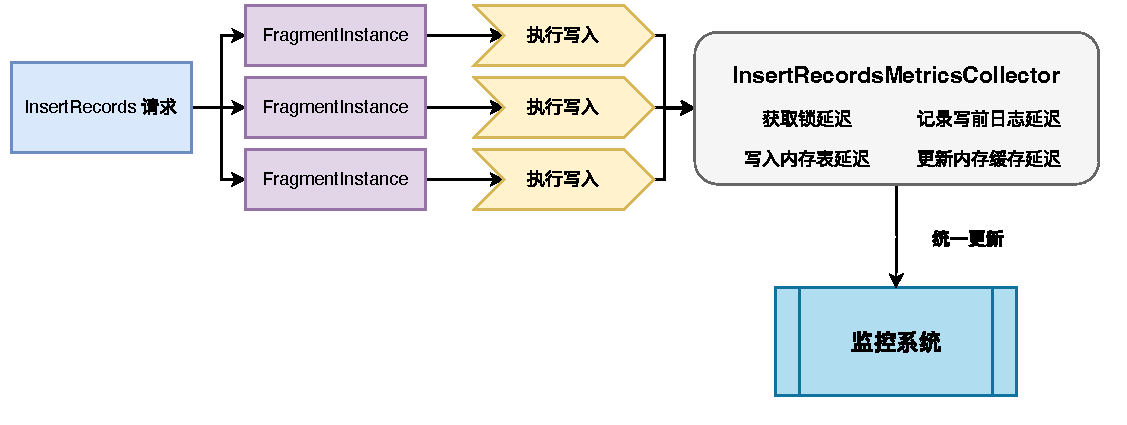
\includegraphics[width=\linewidth]{统一更新监控.pdf}
  \caption{批量化更新监控信息设计}
  \label{fig:batch-update-monitor}
\end{figure}
我们将对监控信息的更新从一行记录更新一次减少为了一个写入请求更新一次,图 \ref{fig:batch-update-monitor} 展示了为了达成这一目的的架构。我们增加了一个名为 InsertRecordsMetricsCollector 的类,这个类的每一个实例都只服务于一个 \emph{insertRecords} 请求。这个类中有若干个 AtomicLong 类型的字段,每个字段分别对应了一个监控指标。每个 FragmentInstance 在执行写入时都会记录自己执行时各个阶段的耗时,并将这些耗时更新到 InsertRecordsMetricsCollector 的对应字段中。当所有 FragmentInstance 都执行完毕以后,主写入线程会将 InsertRecordsMetricsCollector 中的每个字段的值分别更新到监控系统中。

虽然 FragmentInstance 在执行时仍然会多次更新 InsertRecordsMetricsCollector 的字段,但是这些更新都只需要简单的 CAS(Compare And Swap)指令即可完成,而更新监控系统则需要执行对直方图的更新,后者显然更加复杂和耗时。因此,在这样的设计下可以降低写入过程中更新监控信息的开销。
\subsubsection{批量化更新内存缓存}
与批量化更新监控信息类似,我们将更新内存缓存的操作进行了批量化。在更新内存缓存之前,我们会先对 FragmentInstance 中的数据进行排序和去重,保留每个时间序列的最后一个数据点。然后,我们将这些信息一次性更新到内存缓存中,以减少对内存缓存的更新次数。

算法 \ref{alg:batch-update-cache} 展示了批量化更新内存缓存的伪代码。我们使用了一个 Map 来记录每个时间序列的最后一个数据点,最后将这个 Map 中的内容更新到内存缓存中。理论上,LastCache 本身也是一个 Map 结构,但是 LastCache 是一个需要提供全局访问和更新的数据结构,对它的更新会带来同步开销,因此我们选择了先将数据聚集到一个 Map 中,然后再一次性地更新到 LastCache 中,以减少对 LastCache 的更新次数。
\begin{algorithm}
  \caption{批量化更新内存缓存}
  \label{alg:batch-update-cache}
  \small
  \begin{algorithmic}
    \REQUIRE 写入计划分片 FragmentInstance
    \ENSURE LastCache 被更新
    \STATE $n \leftarrow $FragmentInstance.size
    \STATE $lastCache \leftarrow $new HashMap<TimeSeriesId, Pair<Timestamp, Value>>
    \FOR{$i=1$ to $n$}
    \STATE $tsId \leftarrow $FragmentInstance.getTsId($i$)
    \STATE $timestamp \leftarrow $FragmentInstance.getTimestamp($i$)
    \STATE $value \leftarrow $FragmentInstance.getValue($i$)
    \IF{$tsId$ 不在 $lastCache$ 中 \OR $timestamp > lastCache.get(tsId).getKey$}
    \STATE $lastCache.put(tsId, \langle timestamp, value \rangle)$
    \ENDIF
    \ENDFOR
    \STATE 使用 $lastCache$ 更新系统全局的 LastCache
  \end{algorithmic}
\end{algorithm}
\subsubsection{批量化写入内存表}
在正式写入一个 FragmentInstance 之前,我们将这个 FragmentInstance 中的数据按照写入的内存表进行归类。在 IoTDB 中,一个 DataRegion 会为每一个时间分区维护两个内存表,一个写入顺序数据,一个写入乱序数据。因此,我们只要确定每行记录的时间分区范围以及其顺乱序,就可以确定它们要写到哪个内存表,然后将写入一个内存表的数据聚集到一起,一次性地写入到该内存表中。这样的设计有助于减少写入内存表过程中的固定开销,也有助于提高 CPU 缓存的命中率,进而提高写入性能。
\section{写前日志压缩设计与实现\label{sec:chap7-sec4}}
在 \ref{sec:chap3-sec3-1} 的实验中,我们对比了 \emph{insertRecords} 写入和 \emph{insertTablets} 写入所产生的 WAL 大小和数据文件大小的比值,其中 \emph{insertRecords} 的这一比值为 7:1,是 \emph{insertTablets} 的两倍还多。这也就意味着,在 IoTDB 使用 \emph{insertRecords} 进行写入时,有接近 90\% 的 I/O 资源都用于写前日志的写入,这无疑会影响写入性能。

为了减少 WAL 的大小,节省系统的 I/O 资源,我们对写前日志进行了压缩。下面介绍 WAL 压缩的设计与实现。
\subsection{写前日志压缩设计}
\begin{figure}
  \centering
  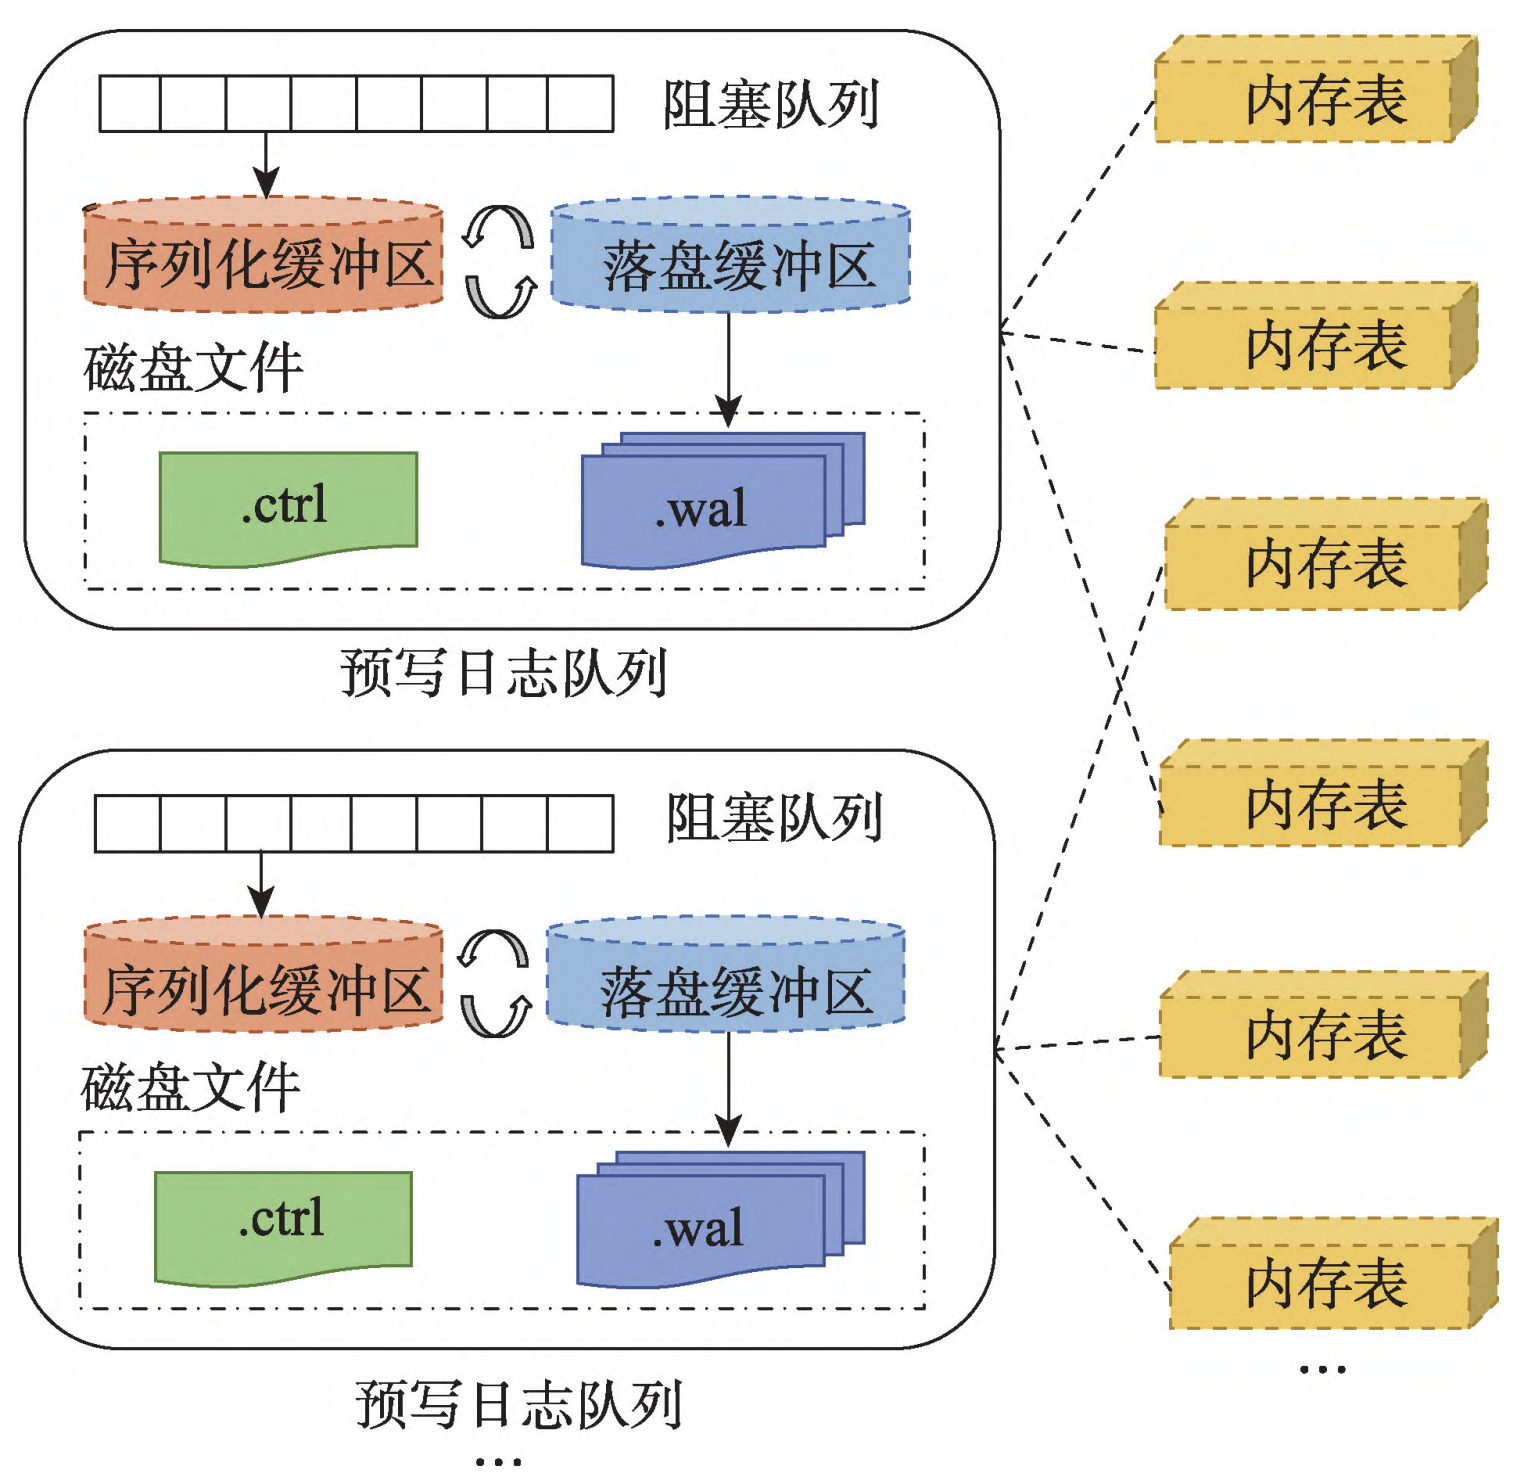
\includegraphics[width=0.7\linewidth]{WAL-structure.png}
  \caption{IoTDB 写前日志结构\cite{朱海铭2023面向内存表的可动态配置预写日志框架}}
  \label{fig:wal-compress-design}
\end{figure}

图 \ref{fig:wal-compress-design} 展示了目前 IoTDB 写前日志系统的结构,多个内存表的写前日志会被写入到同一个 WAL Buffer 中,每个 WAL Buffer 有一个对应的阻塞队列,用于接收异步提交的 WAL 序列化需求。每个 WAL Buffer 都使用了两个内存里的 Buffer 对象来缓存 WAL 序列化后的数据,两个 Buffer 交替使用。当其中一个 Buffer 写满了以后,就会被提交到异步的落盘线程中进行持久化,另一个空 Buffer 则会被用来接收新的 WAL 序列化需求。

对写前日志模块的改动容易牵涉到 IoTDB 中的多个子模块,例如 IoT-Consensus 多副本共识协议、IoTDB 流处理系统都依赖于写前日志中的内容进行数据同步和数据传输。如果按照写前日志项为单位进行压缩,有可能会导致上层应用也需要进行修改,工程量较大。因此,我们的设计需要尽量对上层的应用透明,但是在 I/O 时可以减少写前日志的体积。此外,一个写前日志项序列化出的内容有可能需要多个 WAL Buffer 分别持久化到磁盘上。例如,一个写入中带有 30 MB 的文本,而一个 WAL Buffer 的默认大小是 16 MB,此时该写入请求对应的写前日志就需要通过两个 WAL Buffer 才能完全持久化到磁盘上。在发生这种情况时,针对单一写入日志项的压缩也不易实现。综上,以一个写前日志项为单位的压缩并不是最好的选择,我们选择对整个 WAL Buffer 进行压缩。

对 WAL 的压缩分为两个主要部分:写部分和读部分。在写部分,我们选择在 WAL Buffer 持久化之前对它使用通用压缩算法进行压缩。在读时,需要读取写前日志的模块有存储引擎恢复模块、流处理模块、多副本共识模块等。这些模块对写前日志的读取模式都是先将一块写前日志读入内存,然后解析其中的内容,获取一个个的写前日志项后再继续处理其他上层逻辑。因此,我们在将一个 WAL Buffer 读入内存中时,先将其解压缩,然后将解压缩后的原始 Buffer 进行解析,获取一个个的写前日志项并交由上层应用使用。
\subsection{写前日志压缩实现}
\begin{figure}
  \centering
  
\includegraphics[width=0.7\linewidth]{压缩后WAL的结构.pdf}
  \caption{压缩后的写前日志结构}
  \label{fig:compressed-wal-structure}
\end{figure}
图 \ref{fig:compressed-wal-structure} 展示了压缩后的写前日志结构,我们把这样一个结构称为一个 WAL Segment。在写入时,我们接收到完整的原始 WAL Buffer,然后使用通用压缩算法压缩并记录其原始数据的长度,并且在头部使用一个标记位表示该数据是否被压缩过。之所以需要用标志位,是因为我们把写前日志压缩实现为一个可选的功能。当用户资源不足时,可以不启用写前日志压缩。使用标志位可以保证读取时的兼容性,保证对于压缩和未压缩的写前日志都可以正确解析。

实现压缩的一个关键点是选择合适的压缩算法,IoTDB 目前支持 ZSTD、LZ4、Snappy、LZMA、GZip 等压缩算法。不同压缩算法的压缩率、压缩速度、资源开销各不相同,压缩率越高的往往压缩速度越慢、资源开销越大,反之亦然。经过实验,我们发现 GZip 压缩算法可以取得较好的压缩率和压缩速度,因此我们选择了 GZip 作为 IoTDB 写前日志的压缩算法,具体的实验内容将在第 \ref{sec:chap8} 章中介绍。

在读取时,我们一次读入一个 WAL Segment,然后根据标志位判断是否需要解压缩。如果需要解压缩,就申请一块与原始数据大小相同的内存,然后将压缩后的数据解压缩到这一块内存中,再交由上层应用进行解析。如果不需解压缩,则直接解析 WAL 的数据。这样的设计可以保证对于压缩和未压缩的写前日志都可以正确解析,保证了系统的兼容性。
\section{本章小结}
本章介绍了在存储引擎侧针对 \emph{insertRecords} 写入请求处理进行的若干优化设计,包括多线程并行写入、批量化写入和写前日志压缩。多线程并行写入通过将写入本地 DataRegion 和写入远程 DataRegion 的过程都设计为多线程并行执行,以提高写入性能。批量化写入通过将写前日志、更新监控信息、维护内存索引等操作批量化,减少这些操作对写入性能的影响。写前日志压缩通过对 WAL Buffer 进行压缩,减少写前日志对磁盘的写入量,提高写入性能。
·% !TeX root = ../thuthesis-example.tex

\chapter{实验与分析\label{sec:chap8}}
本章对前文中所提出的优化设计进行实验,验证这些设计的效果。本章首先介绍实验环境,然后验证在客户端将 \emph{insertRecords} 请求转换为 \emph{insertTablets} 请求带来的性能提升,再验证在不能转为 \emph{insertTablets} 请求的场景下各个优化工作对 \emph{insertRecords} 写入带来的性能提升。最后介绍用户负载采样程序和模拟程序,将所有优化点综合在一起,模拟在用户负载下的性能提升。
\section{实验环境}
\begin{table}
  \centering
  \caption{实验环境}
  \begin{tabular}{ll}
    \toprule
    配置名称 & 配置值 \\
    \midrule 
    CPU & I7-11700 8C16T 2.5GHz\\
    内存 & 32G DDR4 3200 Mhz\\
    DataNode 内存 & 28G \\
    ConfigNode 内存 & 2G \\
    机械硬盘 & 希捷 ST-16000NM000J \\
    JDK 版本 & OpenJDK 11.0.22 \\
    操作系统版本 & Ubuntu 20.04.2 LTS,64 位 \\
    网络环境 & 1000 Mbps 局域网 \\
    \bottomrule
  \end{tabular}
  \label{tabular:iotdb-runtime-config}
\end{table}

表 \ref{tabular:iotdb-runtime-config} 展示了测试所用的硬件环境和软件环境。测试机器分为两台,配置均与表格中展示的一致,一台用于运行 IoTDB,另一台则用于运行测试程序。IoTDB 在部署时将一个 DataNode 和一个 ConfigNode 部署到了同一台机器上,DataNode 分配了 28G 的内存,ConfigNode 分配了 2G 的内存。IoTDB 使用了一块希捷 ST-16000NM000J 机械硬盘作为存储设备,系统数据、写前日志、系统运行日志等都会存储在同一块磁盘上。IoTDB 使用了 OpenJDK 11.0.22 作为运行环境,操作系统为 Ubuntu 20.04.2 LTS,64 位。测试机器之间的网络通过 1000 Mbps 的局域网连接。在某些实验中,为了模拟更低的网络带宽,我们使用了 wondershaper 工具限制了网络带宽。

\section{客户端请求格式转换性能试验}
在这一节中,我们测试了在客户端处将 \emph{insertRecords} 请求转换为 \emph{insertTablets} 请求所带来的性能提升。我们使用 IoT Benchmark 作为测试程序,并且将客户端的转换系数设置为 0.5,即只要平均每个设备有 2 条记录,就会转换为 Tablets 进行写入。
\begin{table}
  \centering
  \caption{请求转换格式测试 IoT Benchmark 配置}
  \begin{tabular}{ll}
    \toprule
    配置名称 & 配置值 \\
    \midrule 
    设备数 & 100000 \\
    每个设备的序列数 & 20 \\
    存储组数 & 5 \\
    写入客户端数 & 25 \\
    每个写入请求的行数 & 2000 \\
    \bottomrule
  \end{tabular}
  \label{tabular:test-req-format-iot-benchmark-config}
\end{table}
实验所使用的 IoT Benchmark 配置如表 \ref{tabular:test-req-format-iot-benchmark-config} 所示,实验过程中我们固定每个写入请求的大小为 2000 条记录,但是不断改变每个设备的记录数($records\_per\_device$)和一个请求中的设备数($device\_num$),保证 $records\_per\_device \times device\_num$ 的大小始终等于 2000,观察不同场景下写入性能与原有 \emph{insertRecords} 写入的性能差异。

\begin{figure}
  \centering
  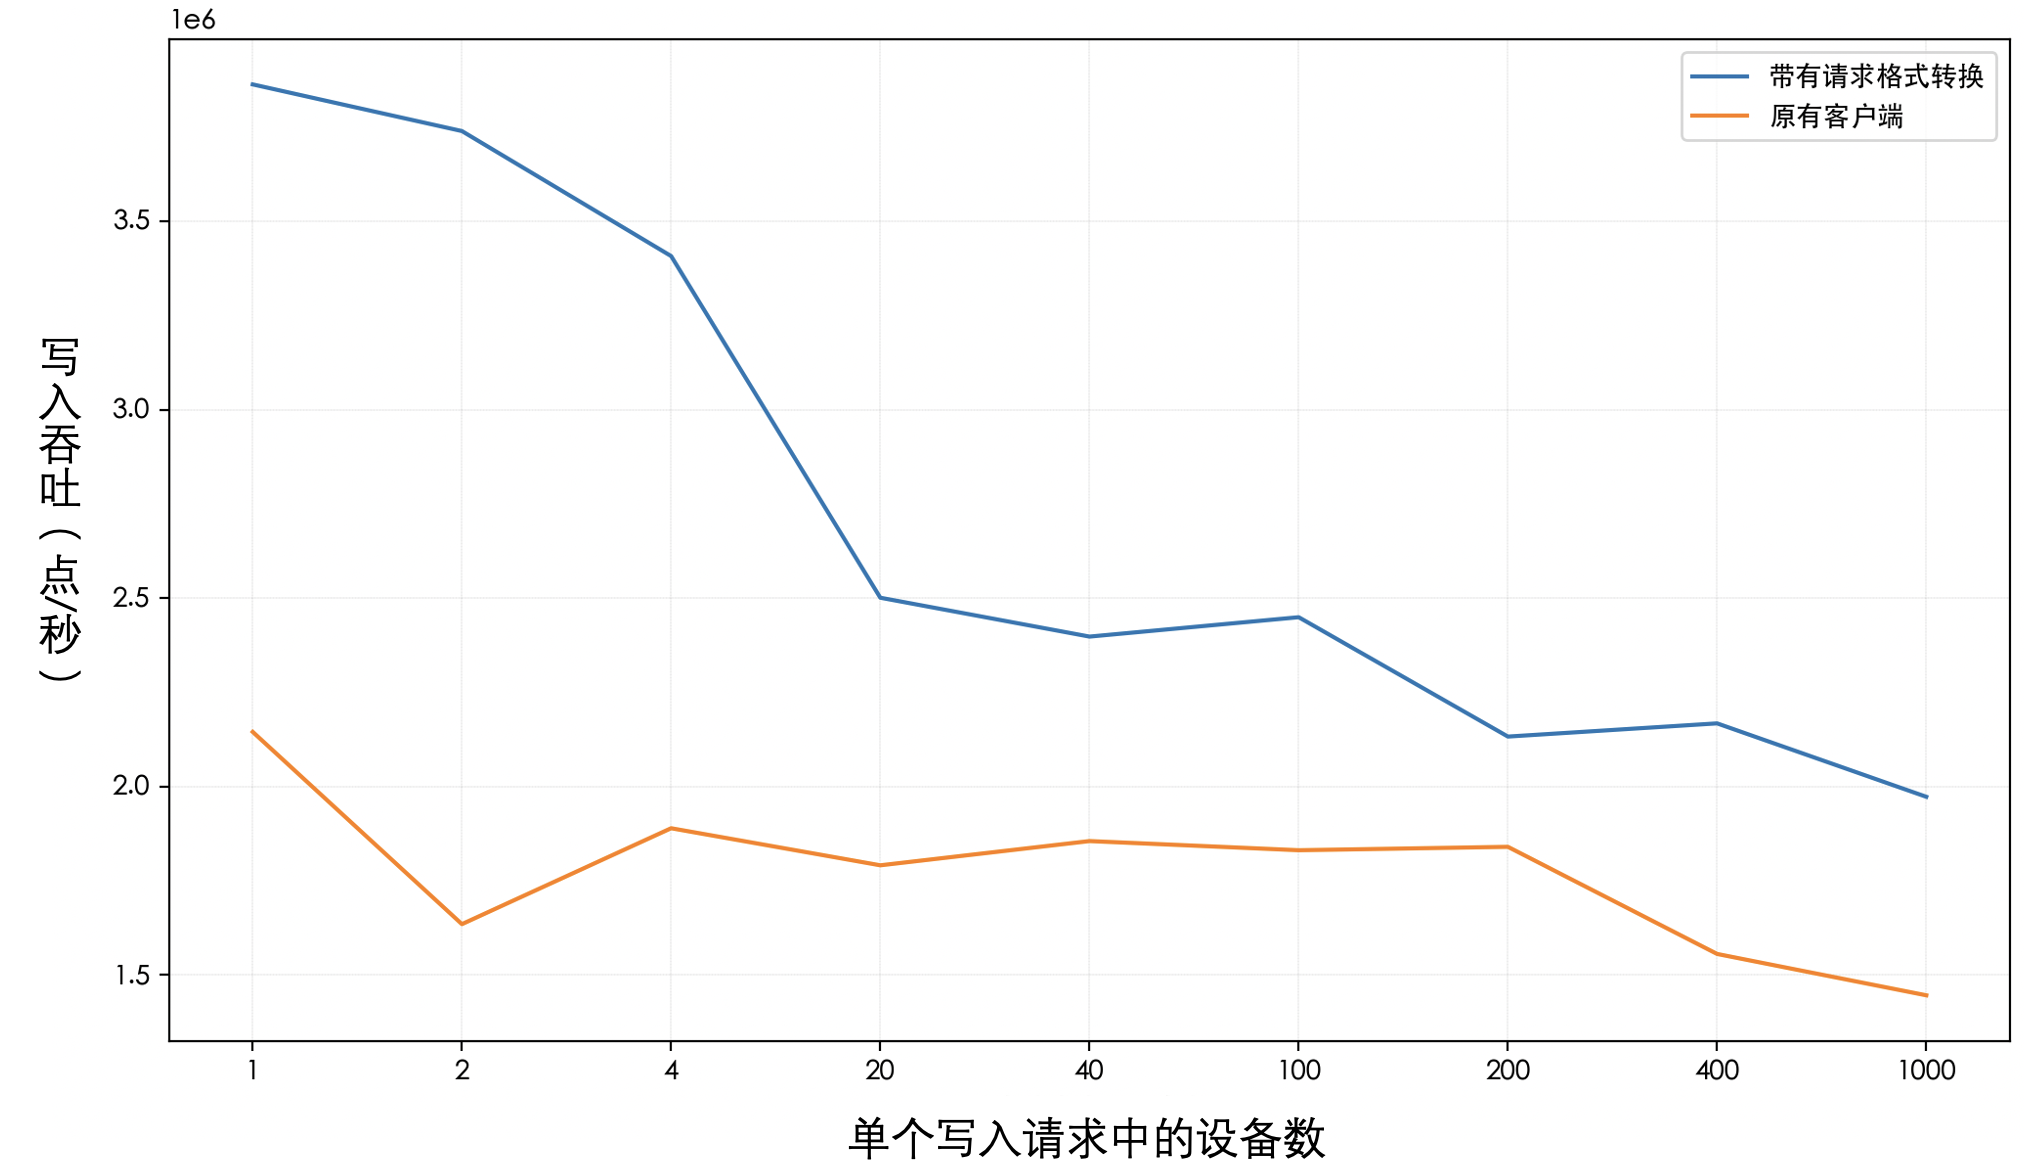
\includegraphics[width=0.8\linewidth]{Records 转换为 Tablets 性能对比.png}
  \caption{客户端请求格式转换实验吞吐量对比}
  \label{fig:records-to-tablets-performance-throughput}
\end{figure}

图 \ref{fig:records-to-tablets-performance-throughput} 展示了单一请求中设备数不同时写入吞吐的对比。客户端进行请求格式转换以后的吞吐显著高于原有客户端,当一个请求中有 2 个设备时,经过请求转换过后吞吐提高了 128\%,在测试的平均情况下提高了 54\% 的写入吞吐。

\begin{figure}
  \centering
  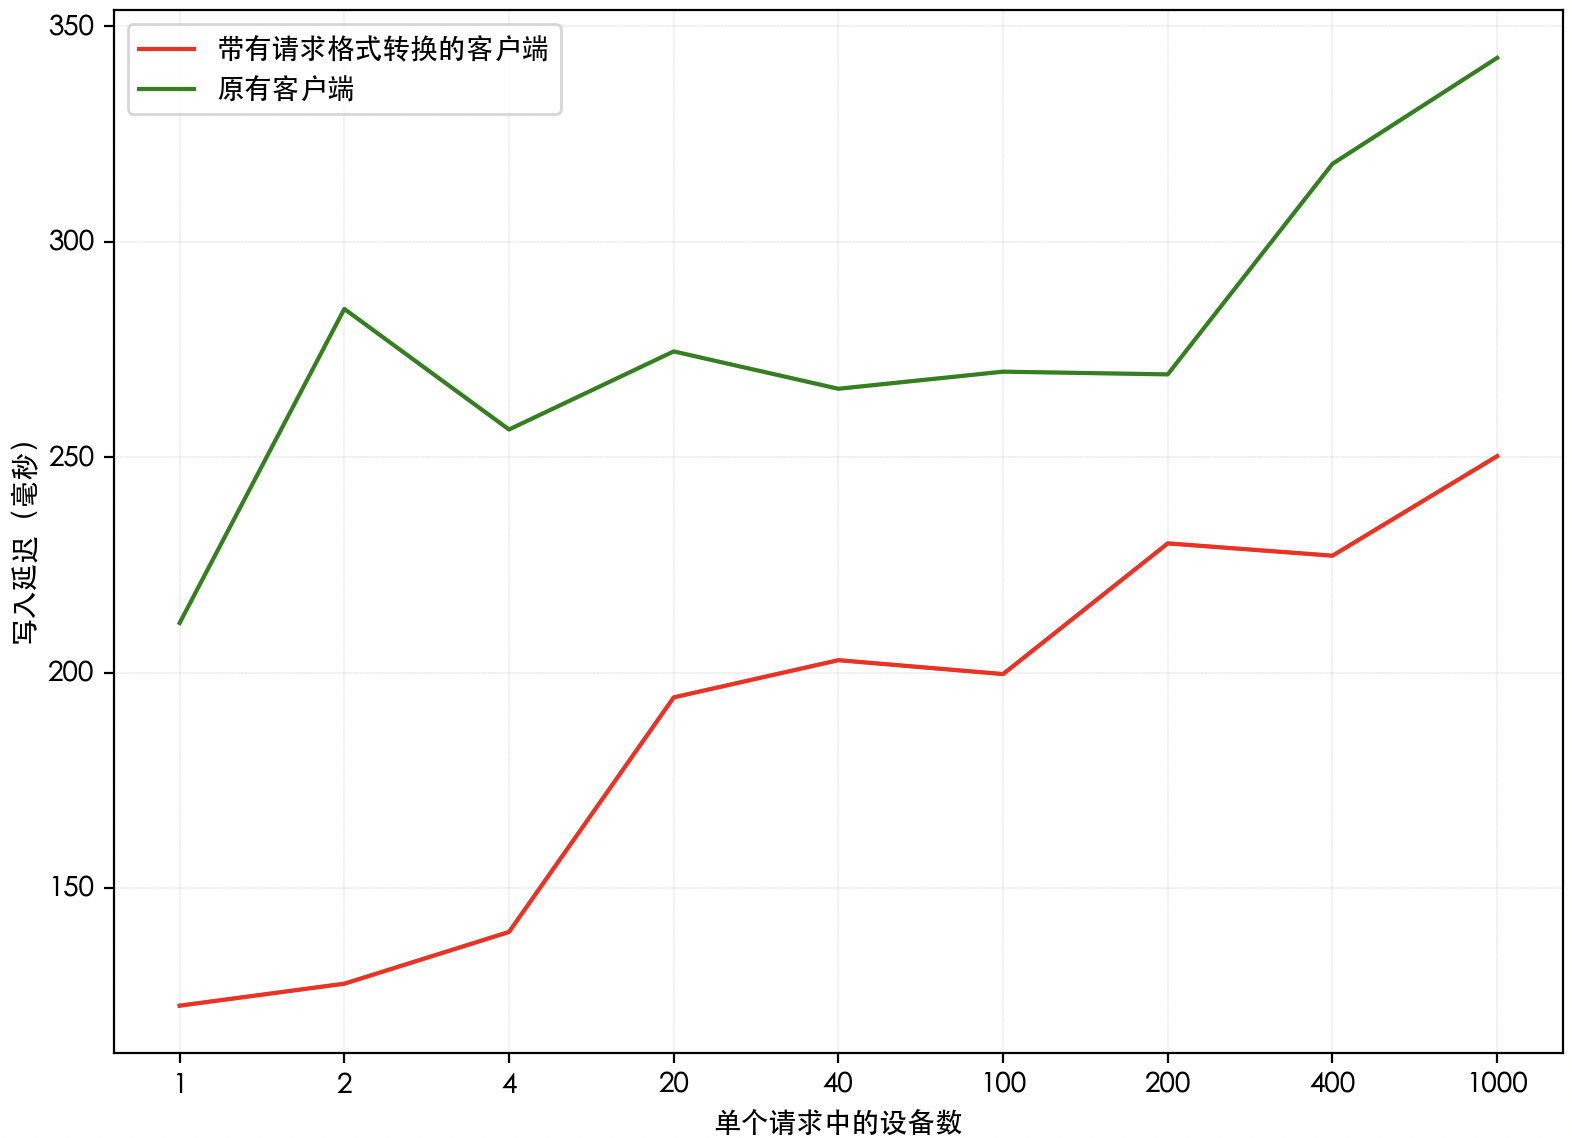
\includegraphics[width=0.7\linewidth]{Records 转 Tablets 平均延迟分布.png}
  \caption{客户端请求格式转换实验平均延迟对比}
  \label{fig:records-to-tablets-performance-avg-latency}
\end{figure}

图 \ref{fig:records-to-tablets-performance-avg-latency} 展示了单一请求中设备数不同时平均写入延迟的对比。客户端进行请求格式转换以后的延迟显著低于原有客户端,当一个请求中有 2 个设备时,经过请求转换过后平均延迟降低了 65.1\%,在测试的平均情况下写入延迟降低了 32.1\%。

\begin{figure}
  \centering
  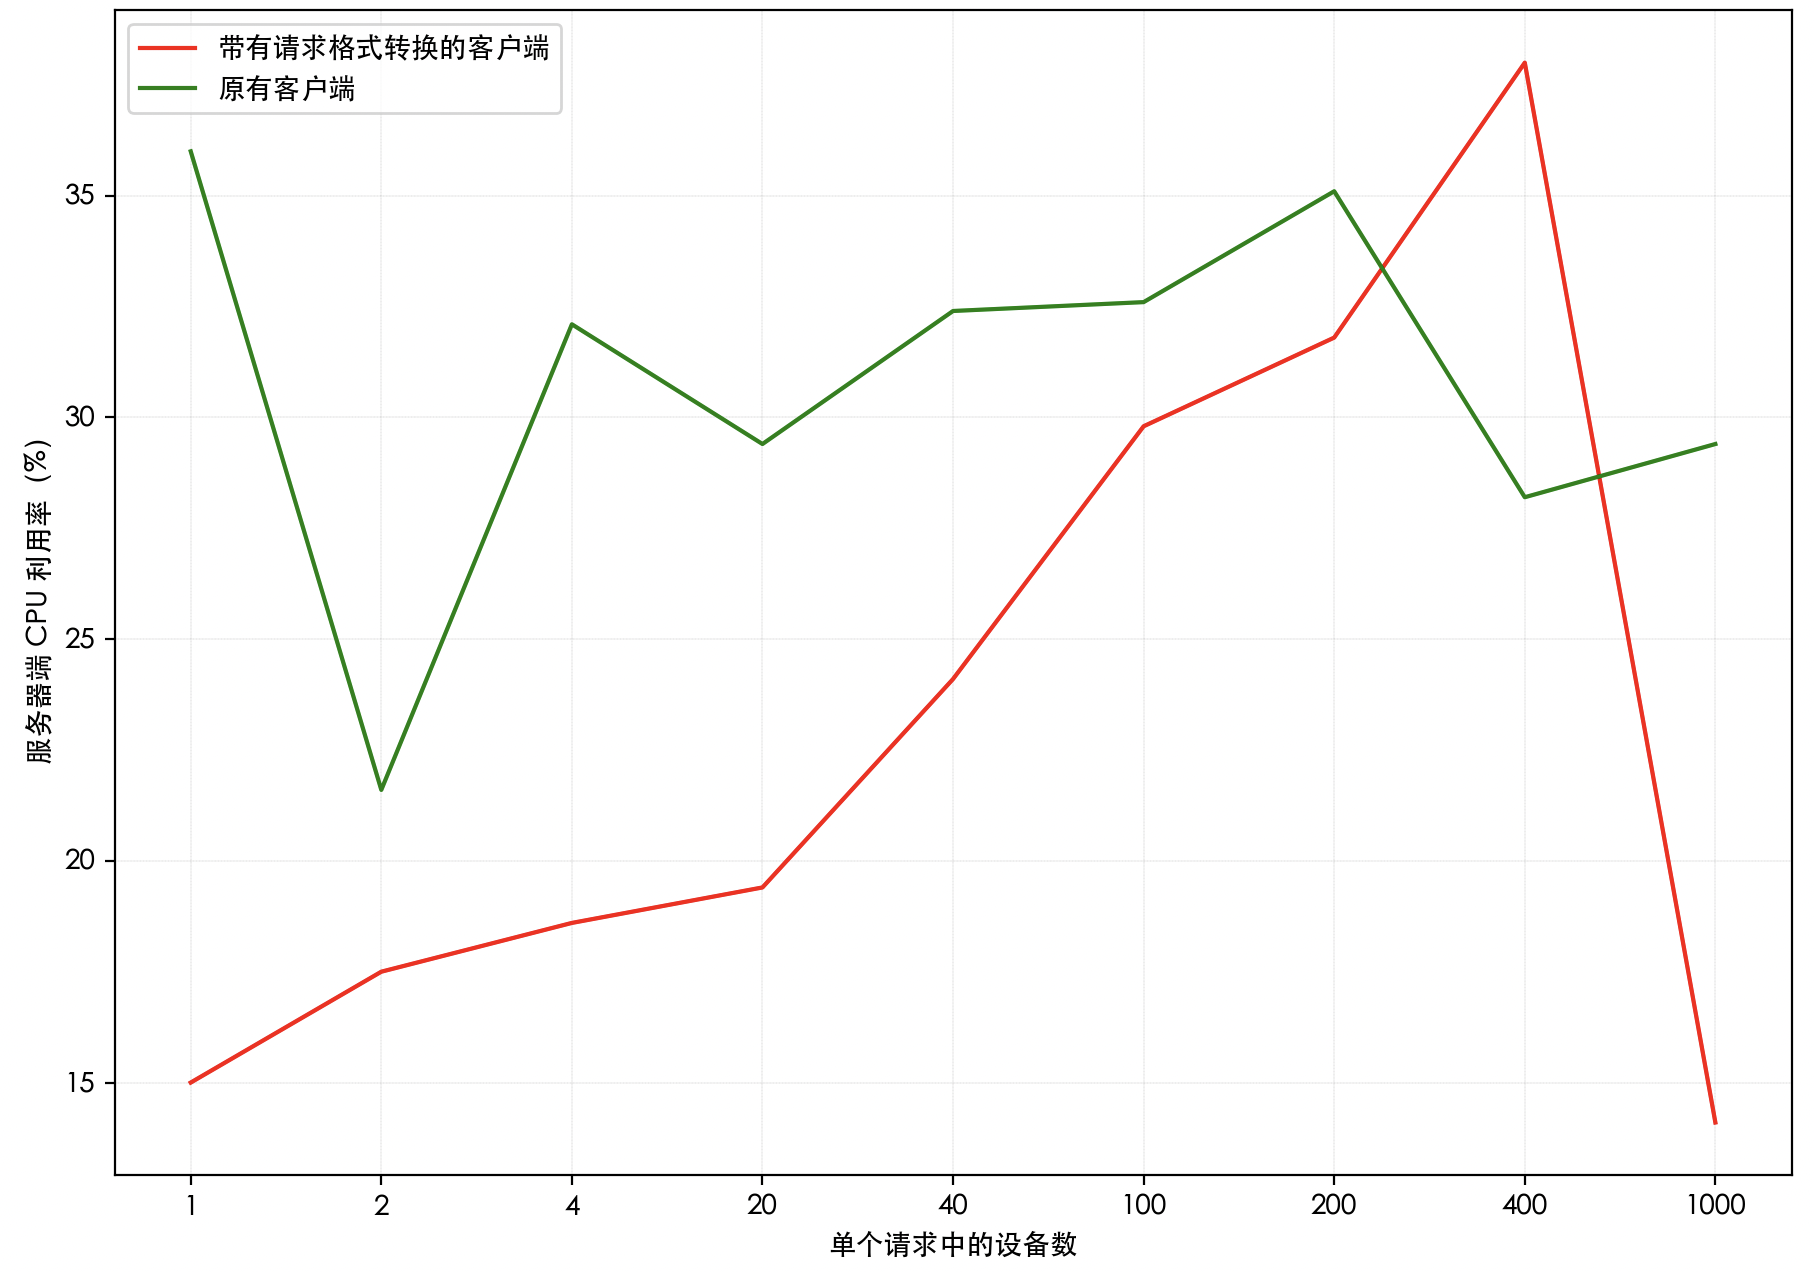
\includegraphics[width=0.7\linewidth]{Records 转 Tablets CPU 资源.png}
  \caption{客户端请求格式转换实验服务区端 CPU 资源消耗对比}
  \label{fig:records-to-tablets-performance-cpu-consuming}
\end{figure}

图 \ref{fig:records-to-tablets-performance-cpu-consuming} 展示了单一请求中设备数不同时服务端 CPU 资源消耗的对比。客户端进行请求格式转换以后的 CPU 资源消耗在大部分情况下显著低于原有客户端,当一个请求中只有 1 个设备时,经过请求转换以后服务器端的 CPU 资源消耗相对降低了 58.3\%,在平均情况下则下降了 24.8\%。但是当一个请求中的设备数为 400 个时,此时经过请求格式转换后服务器的 CPU 资源使用率反而相对上升了 34.7\%。 %TODO:探究原因

实验结果表明,当一个写入请求中每个设备平均有 2 条以上的数据时,在客户端处将它们转换为 \emph{insertTablets} 请求可以显著提高写入的吞吐,降低写入的延迟,并在大部分情况下降低服务器端的资源利用率。这是因为 \emph{insertTables} 本身是一种批量化执行的写入机制,将 \emph{insertRecords} 转换为 \emph{insertTablets} 写入可以在尽量少改动代码的情况下获取较高的收益。因此,在后续的实验中我们关注的是在不能转换为 \emph{insertTablets} 请求的场景下,即每个写入请求中每个设备都只有一条数据的情况下,如何通过其他优化手段提高写入性能。

在后续的实验中,我们先测试对存储引擎的优化所带来的性能提升,并通过实验的结果表明网络带宽已经成为了新的写入性能瓶颈,再测试列式写入序列化在这一场景下所带来的性能提升。最后,我们将所有优化点综合在一起,通过用户负载模拟程序,模拟真实用户的负载,验证所有优化点的综合效果。

\begin{table}
  \centering
  \caption{InsertRecords 写入测试 IoT Benchmark 配置}
  \begin{tabular}{ll}
    \toprule
    配置名称 & 配置值 \\
    \midrule 
    设备数 & 100000 \\
    每个设备的序列数 & 10 \\
    存储组数 & 5 \\
    写入客户端数 & 25 \\
    每个写入请求的设备数 & 1000 \\
    每个写入请求中每个设备的记录数 & 1 \\
    \bottomrule
  \end{tabular}
  \label{tabular:test-req-format-iot-benchmark-config-2}
\end{table}

表 \ref{tabular:test-req-format-iot-benchmark-config-2} 展示了后续实验中所使用的 IoT Benchmark 的配置。在这一配置下,每次写入时每个设备都只写 1 条数据,不会在客户端处被转换为 \emph{insertTablets} 请求,而是仍然会通过 \emph{insertRecords} 请求写入到 IoTDB 中。使用该配置,本工作测试了客户端路径预先校验以及内存预计算对性能的影响,表 \ref{tabular:client-offloading-performance} 展示了实验的结果。从结果中我们可以看出,客户端预先对时间序列 ID 进行校验以及预先计算内存开销后,写入的吞吐提升了 2.2\%,服务器 CPU 的占用下降了 5.2\%,由于写入数据量的提升,其他资源的占用也有所提升。

\begin{table}  
  \centering  
  \caption{客户端时间序列 ID 预校验与内存预计算性能测试结果}  
  \begin{tabular}{cccc}  
    \toprule   
    指标 & 未优化 & 客户端数据预处理 & 变化幅度 \\   
    \midrule  
    吞吐(点/秒) & 1606206 & 1642600 & +2.2\%\\  
    平均延迟(ms) & 321.00 & 313.12 & -2.4\%\\  
    P99 延迟(ms) & 1303.93 & 1769.08 & +35.6\% \\  
    服务器 CPU 消耗 & 44.4\% & 42.1\% & -5.2\%\\  
    服务器磁盘利用率 & 93.2\% & 94.2\% & +1.1\%\\  
    服务器磁盘吞吐(MB/s) & 129 & 134 & +3.9\% \\  
    网络吞吐(MB/s) & 65.4 & 70.6 & +8.0\%\\  
    \bottomrule   
  \end{tabular}  
  \label{tabular:client-offloading-performance}  
\end{table}

\section{存储引擎优化写入性能测试}
本节测试对存储的优化对性能的提升,测试的性能指标包含吞吐、平均延迟、P99 延迟,资源占用指标包含服务器的 CPU 消耗、磁盘利用率、磁盘吞吐以及网络吞吐。

在性能指标中,吞吐越高代表 IoTDB 每秒钟能写入的数据点数越多;平均延迟代表客户端每个写入请求从开始发送到收到响应的平均时间,时间越短代表服务器对单个写入请求处理的速度越快;P99 延迟表示在所有延迟样本中,99\% 的请求延迟都低于或等于这个值,只有 1\% 的请求延迟超过这个值,P99 延迟越小,代表系统对写入请求的处理越稳定。

在资源占用指标中,CPU 消耗以百分比的形式表示,代表一个时间周期中 CPU 工作时间的占比;磁盘利用率代表磁盘在一个时间周期中的工作时间占比;磁盘吞吐和网络吞吐则分别表示磁盘和网卡在一个时间周期中的数据传输速率。在写入相同数据量的情况下,资源占用指标越低,代表系统对资源的要求越低,系统的处理效率越高。
\subsection{存储引擎批量化写入性能测试}
存储引擎批量化写入主要包括批量化更新监控系统、批量化写入内存表、批量化更新内存缓存、批量化序列化写前日志。这四个优化点优化原理是尽可能地将可以一起被写入的数据绑定起来一起写入或操作,从而平摊写入中的一些固定开销,进而提高性能。
\begin{table}
  \centering
  \caption{批量化写入性能测试结果}
  \begin{tabular}{cccc}
    \toprule 
    指标 & 客户端数据预处理 & 批量化写入 & 变化幅度 \\ 
    \midrule  
    吞吐(点/秒) & 1642600 & 1703651 & +3.7\%\\  
    平均延迟(ms) & 313.12 & 295.73 & -5.6\%\\  
    P99 延迟(ms) & 1769.08 & 1237.56 & -30.0\% \\  
    服务器 CPU 消耗 & 42.1\% & 40.1\% & -4.8\%\\  
    服务器磁盘利用率 & 94.2\% & 92.3\% & -2.0\%\\  
    服务器磁盘吞吐(MB/s) & 134 & 130 & -3.0\% \\  
    网络吞吐(MB/s) & 70.6 & 69.1 & -2.1\%\\  
    \bottomrule
  \end{tabular}
  \label{tabular:batch-write-performance}
\end{table}

表 \ref{tabular:batch-write-performance} 展示了批量化写入对性能的提升,吞吐提升了 3.7\%,平均延迟下降了 5.6\%,在吞吐更高的情况下,服务器的 CPU 消耗量还下降了 4.8\%,磁盘的利用率下降了 2.0\%。这表明,在使用批量化写入以后,IoTDB 的执行效率变得更高了,提升了写入性能的同时降低了对部分资源的使用。

\subsection{写前日志压缩}
在表 \ref{tabular:batch-write-performance} 的实验结果中,我们发现 IoTDB 在测试过程中的磁盘利用率始终处于较高的水平,这表明磁盘的写入速度已经成为了写入性能的瓶颈。从 \ref{sec:chap3-sec3-1} 节的实验中我们发现在使用 \emph{insertRecords} 写入时,写前日志造成的 I/O 量是 TsFile 的 7 倍,这表明写前日志占用了大量的 I/O 资源。为了进一步提高写入性能,我们设计了写前日志压缩机制,将写前日志中的数据进行压缩,减少写入磁盘的数据量,从而提高写入性能。

\begin{table}
  \centering
  \caption{写前日志压缩性能测试结果}
  \begin{tabular}{cccc}
    \toprule 
    指标 & 无批量化写入 & 批量化写入 & 变化幅度 \\
    \midrule
    吞吐(点/秒) & 1703651 & 2453969 & +44.1\%\\
    平均延迟(ms) & 295.73 & 203.83 & -31.1\%\\
    P99 延迟(ms) & 1237.56 & 502.55& -59.4\% \\
    服务器 CPU 消耗 & 40.1\% & 	55.3\% & +37.9\%\\
    服务器磁盘利用率 & 92.3\% & 	66.3\% & -28.2\%\\
    服务器磁盘吞吐(MB/s) & 130 & 	74.8 & -42.5\% \\
    网络吞吐(MB/s) & 69.1 & 	99.5 & +43.9\%\\
    \bottomrule 
  \end{tabular}
  \label{tabular:wal-compression-performance}
\end{table}

表 \ref{tabular:wal-compression-performance} 展示了写前日志压缩对性能的提升,吞吐提升了 44.1\%,平均延迟下降了 31.1\%,代表极端情况的 P99 延迟则下降了 59.4\%。在吞吐提升 44.1\% 的情况下,CPU 利用里提升了 37.9\%,这表明同样 CPU 消耗的情况下写入的数据更多了。磁盘资源紧张的情况得到了显著缓解,磁盘利用率下降了 28.2\%,磁盘吞吐下降了 42.5\%,这表明磁盘已经不再是写入的瓶颈。由于写入数据量的增加,网络带宽的占用也从 69.1 MB/s 上升到了 99.5 MB/s。由于测试环境的网络理论带宽为 1000Mbps,此时的网络带宽已经接近了网络的极限,这表明网络带宽已经成为了新的写入性能瓶颈。


\section{写入请求列式序列化性能测试}
从表 \ref{tabular:wal-compression-performance} 展示的试验结果中,我们发现网络可能成为了写入的新瓶颈。为了进一步提高写入性能,我们设计了列式写入请求序列化机制,将写入请求中的数据进行列式序列化,减少写入网络的数据量,从而提高写入性能。

\begin{table}
  \centering
  \caption{列式写入请求序列化性能测试结果}
  \begin{tabular}{cp{3.5cm}p{3.5cm}c}
    \toprule 
    指标 &  无写入请求序列化 & 列式写入请求序列化 & 变化幅度 \\
    \midrule  
    吞吐(点/秒) & 2453969 & 3308927 & +34.4\%\\  
    平均延迟(ms) & 203.83 & 165.48 & -18.8\%\\  
    P99 延迟(ms) & 502.55 & 915.74 & +82.2\%\\  
    服务器 CPU 消耗 & 55.3\% & 65.5\% & +18.4\%\\  
    服务器磁盘利用率 & 66.3\% & 81.7\% & +23.2\%\\  
    服务器磁盘吞吐(MB/s) & 74.8 & 91.1 & +21.8\%\\  
    网络吞吐(MB/s) & 99.5 & 3.06 & -96.9\%\\  
    \bottomrule 
  \end{tabular}
  \label{tabular:columnar-serialization-performance}
\end{table}

表 \ref{tabular:columnar-serialization-performance} 展示了加上列式写入请求序列化的结果,吞吐提升了 34.9\%,平均延迟下降了 18.9\%。但是,由于写入请求序列化会带来编码和解编码的开销,容易让 JVM 发生更频繁的垃圾回收,所以代表极端情况的 P99 延迟反而上升了 82.2\%。在吞吐提升 34.9\% 的情况下,CPU 消耗量上升了 18.4\%,磁盘利用率上升了 23.2\%,磁盘吞吐上升了 21.8\%。网络带宽占用显著下降了 96.9\%,降为原有的 3.1\%,远低于测试环境的网络理论带宽,这表明网络带宽已经不再是写入性能的瓶颈。

\begin{table}
  \centering
  \caption{FragmentInstance 并行写入性能测试结果}
  \begin{tabular}{cp{3.5cm}p{3.5cm}c}
    \toprule 
    指标 &    FI 串行写入 &  FI 并行写入 & 变化幅度 \\
    \midrule  
    吞吐(点/秒) & 	3308927 & 3467967 & +4.8\%\\  
    平均延迟(ms) &  	165.48 & 88.3 & -6.9\%\\  
    P99 延迟(ms) & 	915.74 & 740.23 & -9.1\%\\  
    服务器 CPU 消耗 &  	65.5\% & 73.3\% & +1.9\%\\  
    服务器磁盘利用率 & 	81.7\% & 83.3\% & +1.9\%\\  
    服务器磁盘吞吐(MB/s) & 91.1 & 92.4 & +1.4\%\\  
    网络吞吐(MB/s) & 	3.06 & 3.21 & +4.9\%\\  
    \bottomrule
  \end{tabular}
  \label{tabular:fi-parallel-insert-performance}
\end{table}

表 \ref{tabular:fi-parallel-insert-performance} 展示了增加 Fragment Instance 并行插入对性能的影响。从实验结果中可以看出,Fragment Instance 并行插入以后对吞吐的影响并不显著,只增加了 $4\%$,但对延迟的降低非常显著,达到了 $47\%$。这是因为多个 Fragment Instance 可以同时写入到内存表中,使得每个 DataRegion 几乎都连续不断地在写入数据,相比于串行写入减少了写入主线程的等待时间,因此降低了延迟。但是加入 Fragment Instance 并行写入之后服务器 CPU 利用率提升的比例高于吞吐提升的比例,这意味着 CPU 写入每个数据点的开销增加了。这个现象是合理的,因为加入 Fragment Instance 并行写入以后在写入过程中引入了更多线程切换和同步的开销,导致了资源利用率的下降。但总的来说,在降低延迟方面,Fragment Instance 并行写入有着明显的效果。

最后,表 \ref{tabular:columnar-serialization-performance-vs-origin} 展示了以上三种优化措施综合起来相较于未优化之前在表 \ref{tabular:test-req-format-iot-benchmark-config-2} 负载下带来的性能提升,吞吐提升了 116\%,平均延迟下降了 73\%,P99 延迟下降了 44\%,服务器 CPU 消耗提升了 65\%,服务器磁盘利用率下降了 11\%,磁盘吞吐量减少了 28\%,网络带宽的消耗减少了 95\%。这表明通过对存储引擎和写入请求序列化的优化,IoTDB 的写入性能得到了显著提升,同时也减少了对服务器资源的消耗。

\begin{table}
  \centering
  \caption{综合性能测试结果}
  \begin{tabular}{cccc}
    \toprule 
    指标 &  未优化  & 优化后 & 变化幅度 \\
    \midrule
    吞吐(点/秒) & 1606206 & 3467967 & +115.9\% \\
    平均延迟(ms) & 321.00 & 88.3 & -72.5\% \\
    P99 延迟(ms) & 1303.93 & 740.23 & -43.2\% \\
    服务器 CPU 消耗 & 44.4\% & 73.3\% & +65.1\% \\
    服务器磁盘利用率 & 93.2\% & 83.3\% & -10.6\% \\
    服务器磁盘吞吐(MB/s) & 129 & 92.4 & -28.4\% \\
    网络吞吐(MB/s) & 65.40 & 3.21 & -95.1\% \\
\bottomrule
  \end{tabular}
  \label{tabular:columnar-serialization-performance-vs-origin}
\end{table}

% \begin{table}
%   \centering
%   \caption{综合性能测试结果}
%   \begin{tabular}{ccccc}
%     \toprule 
%     指标 &  未优化  & 优化后 &  优化前每万点资源消耗 & 优化后每万点资源消耗 \\
%     \midrule
%     吞吐(点/秒) & 1606206 & 3467967 &  & \\
%     服务器 CPU 消耗 & 44.4\% & 73.3\% &  0.28\% & 0.21\% \\
%     服务器磁盘利用率 & 93.2\% & 83.3\% &  0.58\% & 0.24\% \\
%     服务器磁盘吞吐(MB/s) & 129 & 92.4 &  0.81 & 0.27\\
%     网络吞吐(MB/s) & 65.40 & 3.21 &  0.41 & 0.01 \\
% \bottomrule
%   \end{tabular}
%   \label{tabular:columnar-serialization-performance-vs-origin2}
% \end{table}

\section{用户模拟负载测试}
本节使用模拟用户场景的负载对写入措施进行优化。本节首先介绍了用户负载的采样程序和模拟运行程序,然后使用中冶赛迪、四维智联和宝武集团三位用户的模拟负载对前文的优化措施进行了测试。
\subsection{负载采样程序}
目前 IoTDB 一共有超过一千家企业用户,这些用户的写入负载特征各异。例如在车联网场景中,设备数通常非常多,每个设备产生数据的频率较低;在工业监控场景中,设备数则相对较少,但每个设备产生数据的频率有可能较高。在同一个场景中,不同设备的数据产生频率、时间序列类型、时间序列数量等也可能有所不同。因此,为了更好地模拟真实用户的负载,本工作设计了一个负载采样程序,用于对用户场景特点进行采样。

负载采样程序的主要功能是通过扫描用户运行 IoTDB 所产生的 TsFile,收集时间序列的特征信息。这些信息包括:
\begin{itemize}
  \item \textbf{不同时间序列类型的比例}:IoTDB 目前支持六种类型的时间序列,分别是 INT32、INT64、FLOAT、DOUBLE、BOOLEAN 和 TEXT。不同时间序列类型的比例对于写入性能有一定影响,例如 TEXT 类型写入需要消耗更大的内存,会产生较大的写前日志,而 BOOLEAN 类型的写入则资源消耗相对较小。
  \item \textbf{时间序列数据的频率分布}:不同时间序列的数据产生频率不同,有的时间序列数据产生频率较高,有的时间序列数据产生频率较低,这是用户负载一个重要的特征。
  \item \textbf{单个设备下时间序列数量的分布}:即使在同一用户场景下,不同设备下时间序列数量也可能相差较大,负载采样程序收集每个设备下时间序列数目的分布信息,为构建负载模拟程序提供参考。
  \item \textbf{对齐时间序列与非对齐时间序列的比例}:IoTDB 目前支持两种序列类型,分别是对齐时间序列和非对齐时间序列。两种时间序列在性能上有所不同,对齐时间序列的写入性能较高,而非对齐时间序列的写入性能较低。负载采样程序收集对齐时间序列和非对齐时间序列的比例信息,为构建负载模拟程序提供参考。
  \item \textbf{时间序列的数值分布}:时间序列数据的值分布对于压缩和编码算法性能有一定的影响,负载模拟程序采集不同数据类型的值分布,为构建负载模拟程序提供参考。
\end{itemize}

\begin{figure}
  \centering
  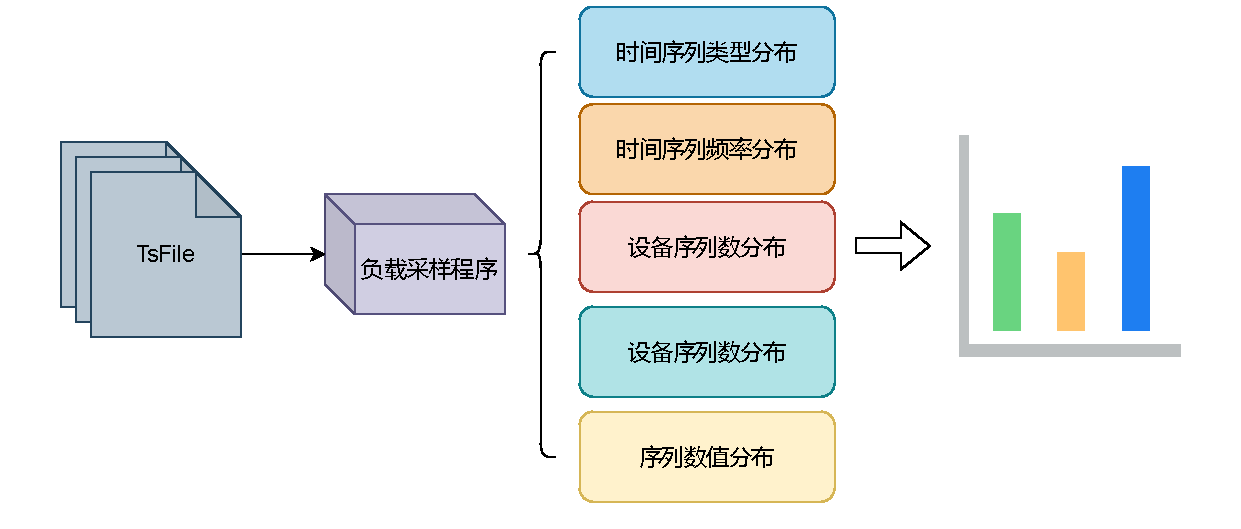
\includegraphics[width=\textwidth]{负载采样程序.pdf}
  \caption{负载采样程序架构}
  \label{fig:load-sampling-program}
\end{figure}

负载采集程序的输入是用户的 TsFile,TsFile 中的数据区分为多个数据块组(ChunkGroup),每个数据块组又分为多个数据块(Chunk)。一个数据块组就对应了一个设备,而一个数据块就对应了一个时间序列的数据。负载采样程序使用 IoTDB 所提供的 TsFileSequenceReader 顺序扫描 TsFile,通过读取每个数据块的数据类型来收集不同时间序列类型的比例,通过读取一个数据块中最大时间点与最小时间点的时间差除以数据点的数目来收集时间序列的频率分布,通过统计每个数据块组下数据块的数目来收集单个设备下时间序列数量的分布,通过读取每个数据块组的类型(对齐或非对齐)来收集对齐时间序列与非对齐时间序列的比例,通过读取每个数据块的数据值来收集不同类型时间序列的数值分布。最后,负载模拟程序将采集到的信息以直方图的形式输出为一个文件,供负载模拟程序使用。

\subsection{负载模拟程序}
图 \ref{fig:load-simulation-program} 展示了模拟负载程序的架构,模拟负载程序接收两个输入,一个是负载采样程序输出的直方图文件,另一个是负载的总设备数。模拟负载程序的运行主要分为两步,第一步是根据直方图和总设备数生成测试的时间序列和设备元数据,第二步则是根据时间序列和设备元数据模拟用户的写入请求。

\begin{figure}
  \centering
  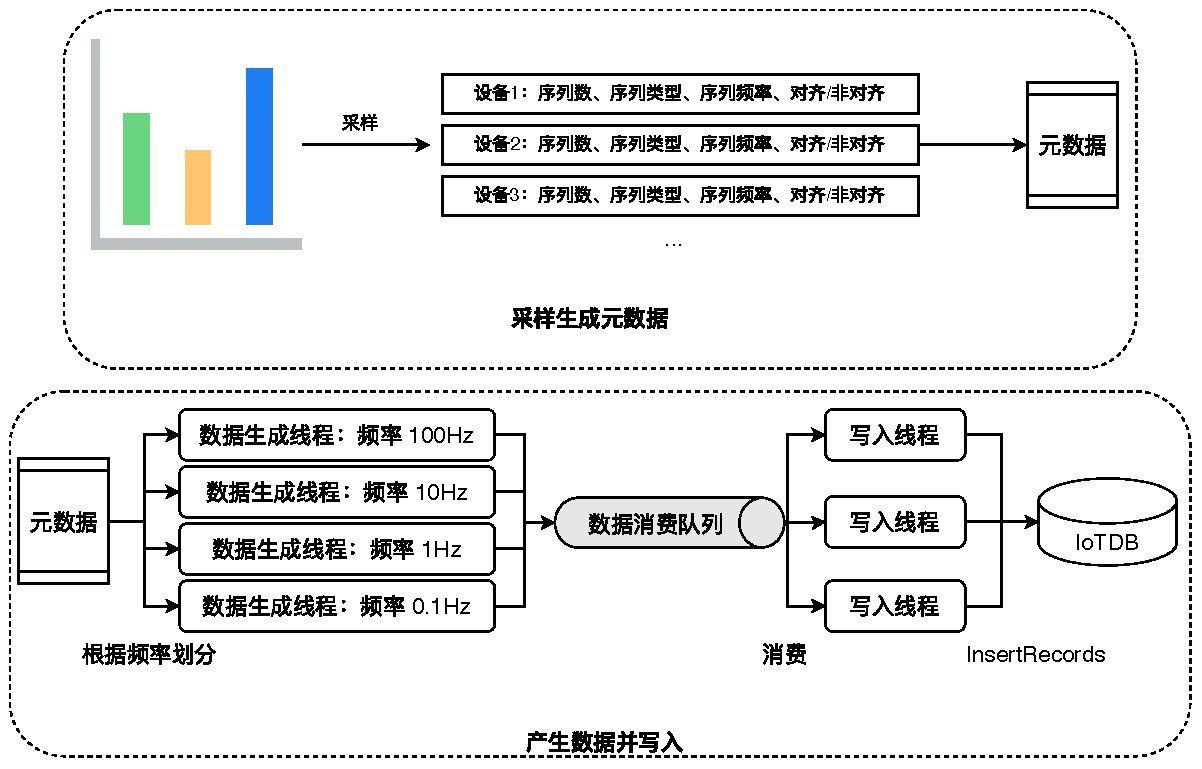
\includegraphics[width=\linewidth]{模拟负载运行程序.pdf}
  \caption{负载模拟程序架构}
  \label{fig:load-simulation-program}
\end{figure}

模拟负载程序运行的第一步是生成测试所需的元数据,这里的元数据既包含了在 IoTDB 中注册时间序列所需的信息,如每个设备下的序列数、序列名称、序列类型,也包含了模拟程序产生数据点所需的信息,如序列的频率、序列的值分布。这些数据的产生通过按照直方图中的分布随机采样得到。一个设备首先会先根据对每个设备下时间序列数的分布进行随机采样,得到本设备的序列数,然后再对频率直方图采样得到本设备下所有时间序列的数据生成频率。然后对于本设备下的每个时间序列,再采样得到其数据类型、值分布等。最后,模拟负载程序一方面将时间序列的元数据注册到 IoTDB 中,另一方面也会将这些信息保存在内存中,用于后续模拟数据的生成和写入。

模拟负载程序运行的第二步是模拟用户的写入请求。模拟负载程序首先会将第一步中生成的设备按照产生数据的频率进行划分,相同频率的设备被归类到一起。然后,具有相同频率的设备会被放到同一个数据生成线程中,这个线程会按照这批设备的频率周期性地按照每个设备的值分布产生数据。如果某一个频率的设备数过多,使用一个线程有可能导致无法按照规定的周期产生数据。例如,如果有大量 100 Hz 的设备,理论上每个设备每隔 10 ms 就要产生一批数据,但是一个线程有可能无法在 10 ms 内产生所有设备的数据,这就会导致最终设备生成数据的频率小于 100 Hz。为了避免这样的情况,每个线程最多负责 5000 个设备的数据生成。这样,即使设备数较多,也可以保证每个设备的数据生成频率不会受到影响。每个数据生成线程会将周期性产生的数据放入一个有限大小的内存并发队列中等待写入线程的消费,如果队列满了就会放弃将数据放入队列,并通过日志记录这种情况。写入队列会不断地从队列中取出数据并在本地缓存生成一个写入请求,如果写入请求的记录行数超过 2000 条或者该写入请求中最旧的数据点的时间戳距离当前时间超过 10 秒,就会将该写入请求通过 \emph{insertRecords} 接口写入到 IoTDB 中。写入线程的数量可以进行调节,以模拟不同的场景。在这样的设计下,模拟负载程序可以容忍 IoTDB 一定的写入延迟波动,从而更好地模拟真实用户的负载。
\subsection{测试负载描述}
利用负载采样程序和负载模拟程序,我们分析了中冶赛迪、四维智联、宝武钢铁集团三家用户的负载,构建了这三家用户的模拟负载程序。
\begin{figure}
  \centering
  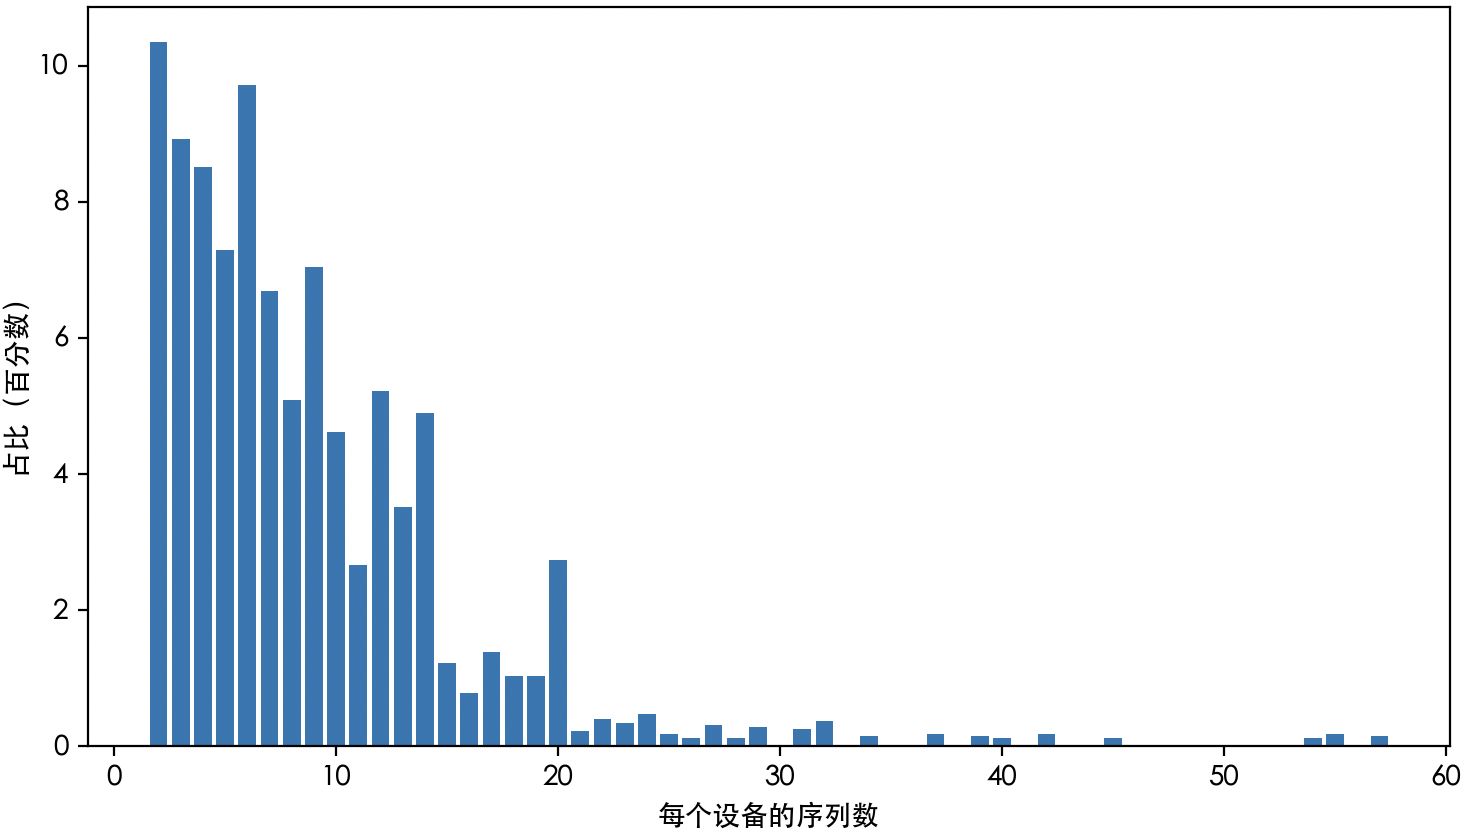
\includegraphics[width=0.7\linewidth]{中冶赛迪-镔鑫项目设备序列数分布图.png}
  \caption{中冶赛迪-镔鑫项目设备序列数分布图}
  \label{fig:zysd-bx-device-measurement-count}
\end{figure}

中冶赛迪模拟负载包含了 20 万个设备与 353.2 万条时间序列,其设备序列数分布如图 \ref{fig:zysd-bx-device-measurement-count} 所示,时间序列的频率分布如图 \ref{fig:zysd-bx-freq-distribution} 所示。中冶赛迪镔鑫负载中大部分序列都是 1 秒产生一个时间点,少量序列几百秒才产生一次数据,极少数序列每隔一百毫秒就会产生一个数据点。每个设备的时间序列数量主要为 2-15 个。根据时间序列数与序列的频率计算,理想情况下数据库需要写入 3391316 个数据点。

\begin{figure}
  \centering
  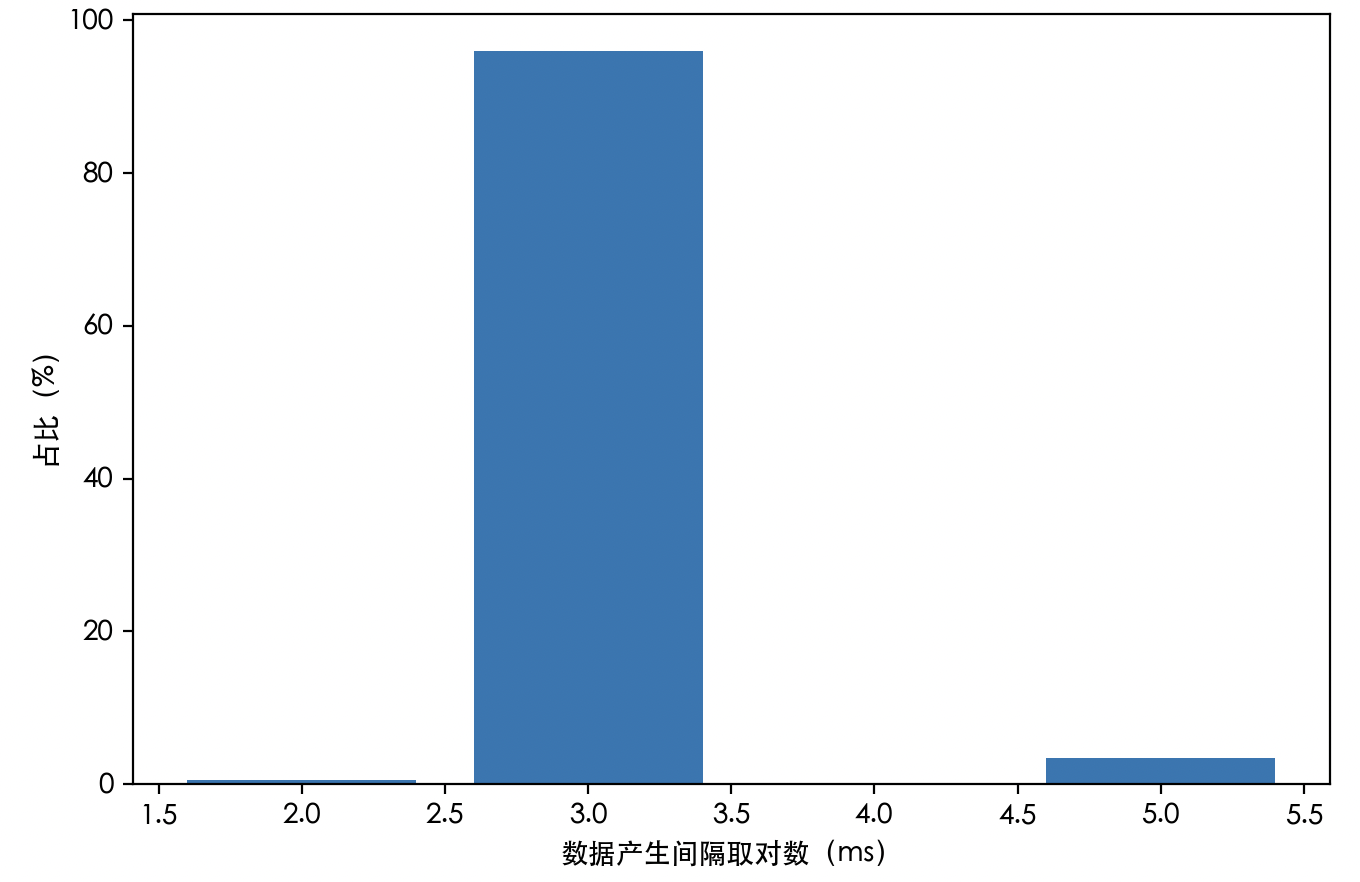
\includegraphics[width=0.7\linewidth]{中冶赛迪镔鑫项目频率分布.png}
  \caption{中冶赛迪-镔鑫项目时间序列频率分布图}
  \label{fig:zysd-bx-freq-distribution}
\end{figure}


\begin{figure}
  \centering
  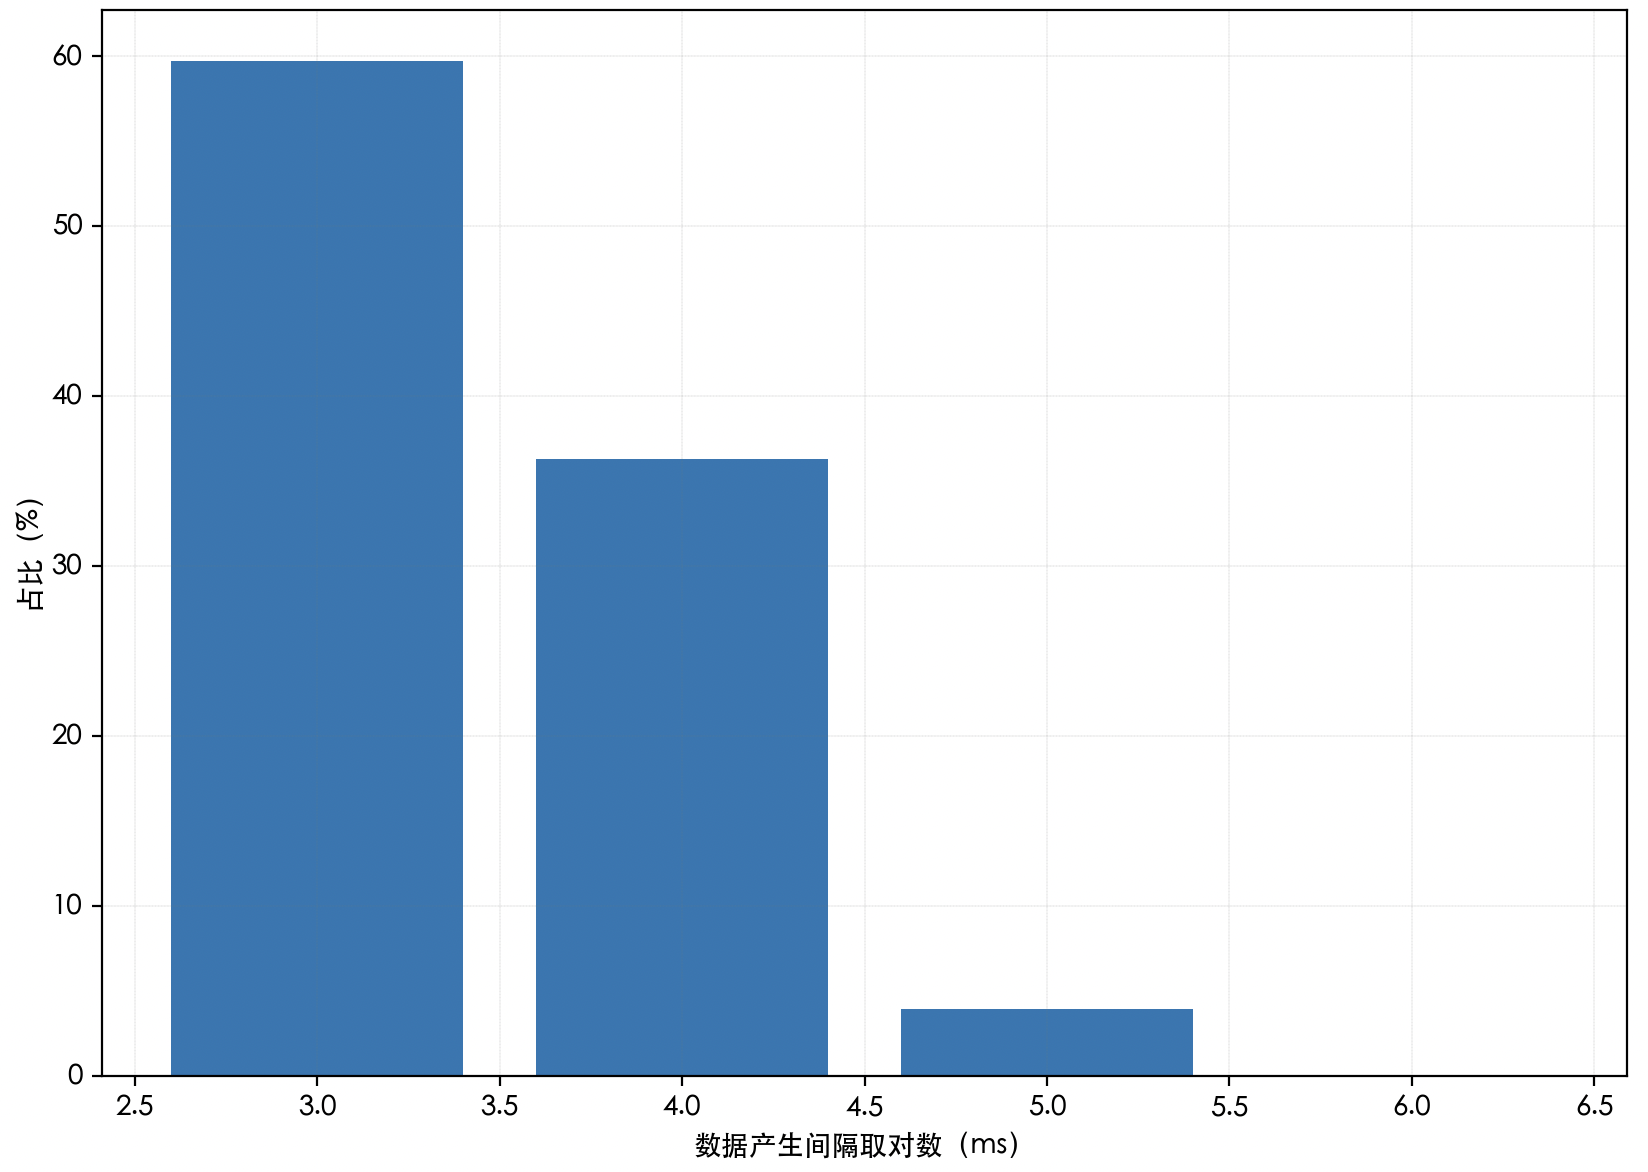
\includegraphics[width=0.7\linewidth]{四维智联时间序列频率分布.png}
  \caption{四维智联时间序列频率分布图}
  \label{fig:swzl-freq-distribution}
\end{figure} 

四维智联的负载每个设备下都有 27 条时间序列,其频率分布如图 \ref{fig:swzl-freq-distribution} 所示,其中超过一半的序列每隔 1 秒钟就会产生一个数据点,大约 35\% 的序列每隔 10 秒才会产生一次数据点,剩下的序列每隔 100 秒才会产生一次数据点。其包含了 25 万个设备和 675 万条时间序列,按照数据产生的频率计算,每秒钟应该写入 1110330 个数据点。


宝武集团的负载特征如图 \ref{fig:bw-freq-distribution} 所示,时间序列由少量极高频(每隔 $10^{-2}$ 毫秒就产生一个数据点)和大量低频(每隔 100 秒才产生一个数据点)以及一些中频(每隔几秒或几十秒产生一个数据点)组成。宝武负载中每个设备包含 1 条或 3 条时间序列,相较于其他负载每个设备下时间序列的数量较少。整个模拟负载包含 25 万个设备和 267516 条时间序列,根据序列数量和序列的频率计算,理想情况下每秒钟应该写入 1410360 个数据点。

\begin{figure}
  \centering
  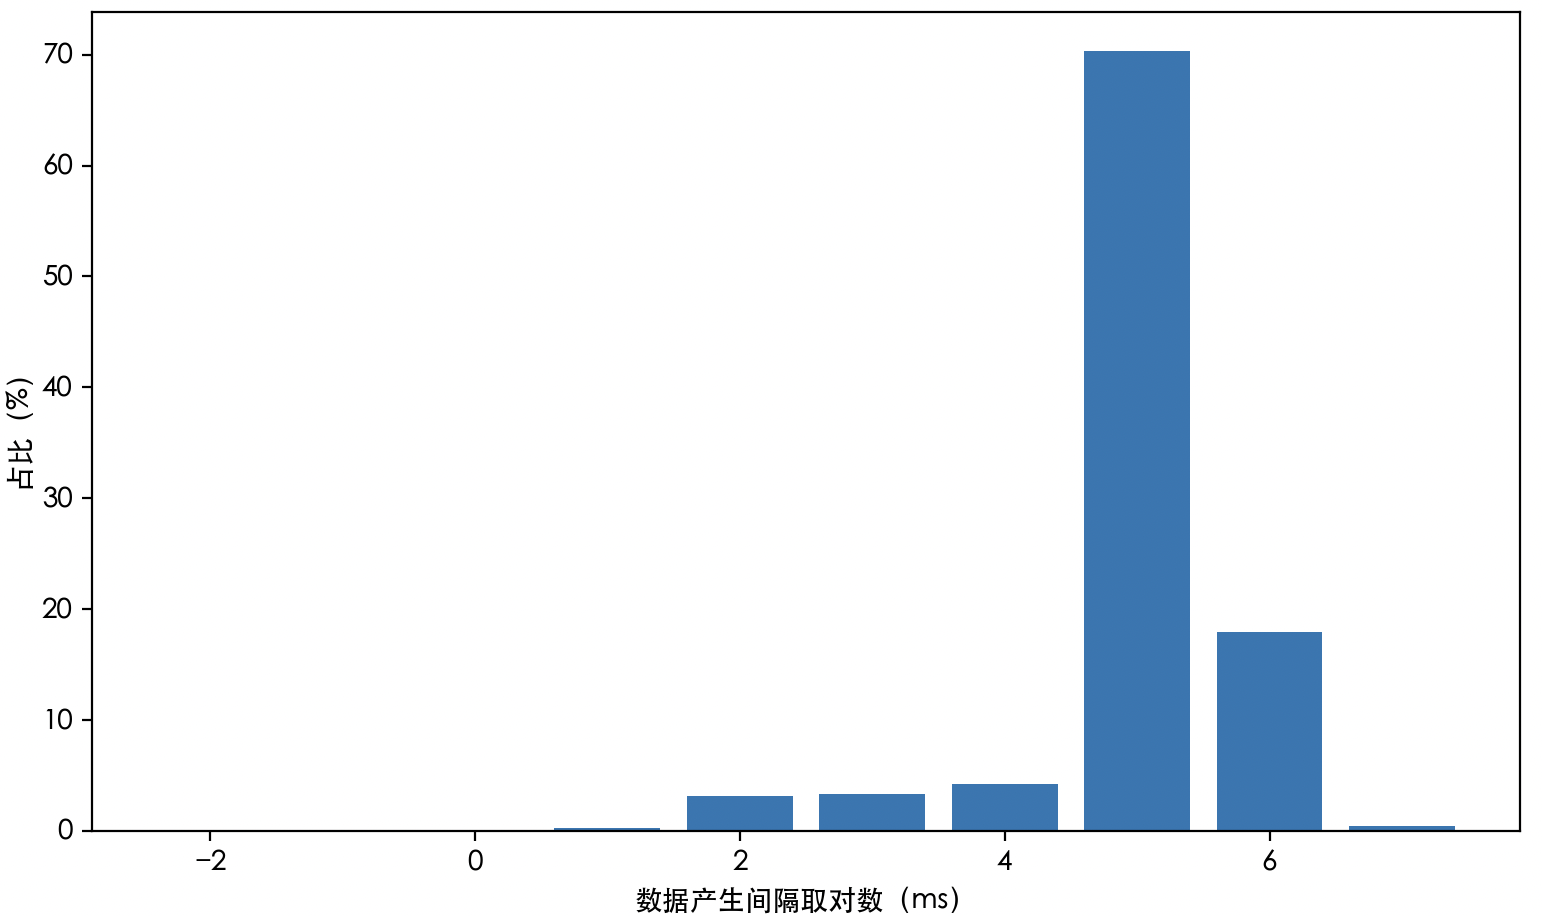
\includegraphics[width=0.7\linewidth]{宝武集团时间序列频率分布.png}
  \caption{宝武集团时间序列频率分布图}
  \label{fig:bw-freq-distribution}
\end{figure}


以上三个用户场景构成了模拟负载的集合,我们将使用这些负载来测试前文的优化措施对 IoTDB 写入性能的提升。 
\subsection{测试结果}

\begin{table}
  \centering
  \caption{中冶赛迪-镔鑫项目模拟测试结果}
  \begin{tabular}{cccc}
    \toprule 
    指标 &  未优化  & 优化后 & 变化幅度 \\
    \midrule
    吞吐(点/秒) & 3392313 & 3391449 & -0.1\%\\
    平均延迟(ms) & 226 & 	117 & -48.2\%\\
    服务器 CPU 消耗 & 61.9\% & 	49.0\% & -20.8\%\\
    服务器磁盘利用率 & 60.8\% & 	33.3\% & -45.2\%\\
    服务器磁盘吞吐(MB/s) & 90.9 & 32.2 & -64.6\% \\
    网络吞吐(MB/s) & 46.4 & 38.1 & -17.9\%\\
    \bottomrule
  \end{tabular}
  \label{tabular:zysd-test-result}
\end{table}
表 \ref{tabular:zysd-test-result} 展示了中冶赛迪-镔鑫模拟负载下 IoTDB 优化前后的性能差异。优化前后的 IoTDB 都可以满足该负载的写入需求,但优化后的 IoTDB 在满足该负载写入请求的情况下平均写入延迟下降了 48\%,CPU、磁盘和网络资源的消耗分别减少了 21\%、46\% 和 18\%。这说明优化后的 IoTDB 在这一场景下处理写入请求的效率更高,因此消耗的资源更少。


\begin{table}
  \centering
  \caption{四维智联负载模拟测试结果}
  \begin{tabular}{cccc}
    \toprule 
    指标 &  未优化  & 优化后 & 变化幅度 \\
    \midrule  
    吞吐(点/秒) & 1108262 & 1112883 & +0.4\%\\  
    平均延迟(ms) & 242 & 165 & -31.8\%\\  
    服务器 CPU 消耗 & 17.4\% & 16.5\% & -5.2\%\\  
    服务器磁盘利用率 & 25.8\% & 16.0\% & -38.0\%\\  
    服务器磁盘吞吐(MB/s) & 37.2 & 17.0 & -54.3\% \\  
    网络吞吐(MB/s) & 16.7 & 5.34 & -68.0\%\\  
    \bottomrule 
  \end{tabular}
  \label{tabular:swzl-test-result}
\end{table}
表 \ref{tabular:swzl-test-result} 展示了在四维智联模拟负载下 IoTDB 优化前后的性能对比,由于四维智联负载压力并不高,优化前后的 IoTDB 都可以满足这个负载的写入需求,但优化优化后 IoTDB 的写入延迟低了 31.8\%。但是在资源占用上,优化后的 IoTDB 的 CPU、磁盘和网络资源消耗的比优化前少了 5.2\%、38.0\%、68.0\%,这表明在完成相同写入的情况下优化后的 IoTDB 资源占用更少,用户在配置服务器时可以选择较低的配置,节约成本。

\begin{table}
  \centering
  \caption{宝武负载模拟测试结果}
  \begin{tabular}{cccc}
    \toprule 
    指标 &  未优化  & 优化后 & 变化幅度 \\
    \midrule
    吞吐(点/秒) & 772071 & 1410360 & +82.7\%\\  
    平均延迟(ms) & 63.4 & 118 & +86.1\%\\  
    服务器 CPU 消耗 & 69.0\% & 35.9\% & -48.0\%\\  
    服务器磁盘利用率 & 40.9\% & 16.6\% & -60.1\%\\  
    服务器磁盘吞吐(MB/s) & 55.2 & 8.07 & -85.3\% \\  
    网络吞吐(MB/s) & 35.4 & 17.3 & -51.1\%\\ 
    \bottomrule
  \end{tabular}
  \label{tabular:bw-performance}
\end{table}
表 \ref{tabular:bw-performance} 展示了在宝武模拟负载的场景下,IoTDB 在优化前后的性能表现。在优化之前,IoTDB 未能满足宝武模拟负载的写入需求,而在优化之后 IoTDB 则可以满足其写入需求。优化后的 IoTDB 写入吞吐是优化前的 1.81 倍,服务器的 CPU、磁盘和网络资源消耗的比优化前少了 48\%、60\% 和 51\%。在这个场景下,一个写入请求中的每一行记录都只有 1 个或 3 个数据点,因此相对而言写入内存表等开销较低。但是,其他部分的开销降低了以后就意味着写入线程会频繁地向写前日志项队列中放入写前日志项,当写前日志项队列满了以后就会阻塞写入线程,造成新的瓶颈。在未优化之前,IoTDB 每一行记录都会产生一个写前日志项,在优化之后一个 FragmentInstance 才会产生一个写前日志项,日志项的数量大大降低,因此可以解除写前日志项队列所造成的瓶颈。

综合以上模拟用户场景的测试结果,在中冶赛迪-镔鑫模拟负载和四维智联模拟负载中,优化前后的 IoTDB 都可以满足负载的写入需求,但优化后的 IoTDB 占用的资源更少,写入效率更高,在对应的真实场景中可以帮助用户节约机器资源,降低生产成本;在宝武集团的模拟负载中,未优化的 IoTDB 无法满足该场景的写入需求,而优化后的 IoTDB 则可以很好地满足需求,并且占用的资源也更少。这表明,经过本工作优化后 IoTDB 的 \emph{insertRecords} 写入机制性能和效率都得到了提升,实现了本工作的目标。
\section{本章小结}
本章首先使用 IoT Benchmark 测试了当一个写入请求中每个设备有多条记录的情况下将 \emph{insertRecords} 转换为 \emph{insertTablets} 所带来的性能提升,然后测试了每个设备都只有一行记录的情况下无法转换为 \emph{insertTablets} 时,写前日志压缩、批量化写入、写入请求列式序列化、Fragment Instance 并行写入等优化点对于写入性能的提升。最后,本章介绍了本工作开发的用户负载采样程序和模拟运行程序,验证了在中冶赛迪、四维智联和宝武集团三家用户的模拟负载下本工作的优化措施对 IoTDB 写入性能的提升。
% !TeX root = ../thuthesis-example.tex

\chapter{总结与展望}


% 其他部分
\backmatter

% 参考文献
\bibliography{ref/refs}  % 参考文献使用 BibTeX 编译
% \printbibliography       % 参考文献使用 BibLaTeX 编译

% 附录
% 本科生需要将附录放到声明之后,个人简历之前
\appendix
% % !TeX root = ../thuthesis-example.tex

\begin{survey}
\label{cha:survey}

\title{Title of the Survey}
\maketitle


\tableofcontents


本科生的外文资料调研阅读报告。


\section{Figures and Tables}

\subsection{Figures}

An example figure in appendix (Figure~\ref{fig:appendix-survey-figure}).

\begin{figure}
  \centering
  
\includegraphics[width=0.6\linewidth]{example-image-a.pdf}
  \caption{Example figure in appendix}
  \label{fig:appendix-survey-figure}
\end{figure}


\subsection{Tables}

An example table in appendix (Table~\ref{tab:appendix-survey-table}).

\begin{table}
  \centering
  \caption{Example table in appendix}
  \begin{tabular}{ll}
    \toprule
    File name       & Description                                         \\
    \midrule
    thuthesis.dtx   & The source file including documentaion and comments \\
    thuthesis.cls   & The template file                                   \\
    thuthesis-*.bst & BibTeX styles                                       \\
    thuthesis-*.bbx & BibLaTeX styles for bibliographies                  \\
    thuthesis-*.cbx & BibLaTeX styles for citations                       \\
    \bottomrule
  \end{tabular}
  \label{tab:appendix-survey-table}
\end{table}


\section{Equations}

An example equation in appendix (Equation~\eqref{eq:appendix-survey-equation}).
\begin{equation}
  \frac{1}{2 \uppi \symup{i}} \int_\gamma f = \sum_{k=1}^m n(\gamma; a_k) \mathscr{R}(f; a_k)
  \label{eq:appendix-survey-equation}
\end{equation}


\section{Citations}

Example citations in appendix.
\cite{abrahams99tex}
\cite{salomon1995advanced}
\cite{abrahams99tex,salomon1995advanced}


\bibliographystyle{unsrtnat}
\bibliography{ref/appendix}

\end{survey}
       % 本科生:外文资料的调研阅读报告
% % !TeX root = ../thuthesis-example.tex

\begin{translation}
\label{cha:translation}

\title{书面翻译题目}
\maketitle

\tableofcontents


本科生的外文资料书面翻译。


\section{图表示例}

\subsection{图}

附录中的图片示例(图~\ref{fig:appendix-translation-figure})。

\begin{figure}
  \centering
  
\includegraphics[width=0.6\linewidth]{example-image-a.pdf}
  \caption{附录中的图片示例}
  \label{fig:appendix-translation-figure}
\end{figure}


\subsection{表格}

附录中的表格示例(表~\ref{tab:appendix-translation-table})。

\begin{table}
  \centering
  \caption{附录中的表格示例}
  \begin{tabular}{ll}
    \toprule
    文件名          & 描述                         \\
    \midrule
    thuthesis.dtx   & 模板的源文件,包括文档和注释 \\
    thuthesis.cls   & 模板文件                     \\
    thuthesis-*.bst & BibTeX 参考文献表样式文件    \\
    thuthesis-*.bbx & BibLaTeX 参考文献表样式文件  \\
    thuthesis-*.cbx & BibLaTeX 引用样式文件        \\
    \bottomrule
  \end{tabular}
  \label{tab:appendix-translation-table}
\end{table}


\section{数学公式}

附录中的数学公式示例(公式\eqref{eq:appendix-translation-equation})。
\begin{equation}
  \frac{1}{2 \uppi \symup{i}} \int_\gamma f = \sum_{k=1}^m n(\gamma; a_k) \mathscr{R}(f; a_k)
  \label{eq:appendix-translation-equation}
\end{equation}


\section{文献引用}

文献引用示例\cite{abrahams99tex}。


\appendix

\section{附录}

附录的内容。


% 书面翻译的参考文献
\bibliographystyle{unsrtnat}
\bibliography{ref/appendix}

% 书面翻译对应的原文索引
\begin{translation-index}
  \nocite{salomon1995advanced}
  \bibliographystyle{unsrtnat}
  \bibliography{ref/appendix}
\end{translation-index}

\end{translation}
  % 本科生:外文资料的书面翻译
% !TeX root = ../thuthesis-example.tex

\chapter{补充内容}

附录是与论文内容密切相关、但编入正文又影响整篇论文编排的条理和逻辑性的资料,例如某些重要的数据表格、计算程序、统计表等,是论文主体的补充内容,可根据需要设置。

附录中的图、表、数学表达式、参考文献等另行编序号,与正文分开,一律用阿拉伯数字编码,
但在数码前冠以附录的序号,例如“图~\ref{fig:appendix-figure}”,
“表~\ref{tab:appendix-table}”,“式\eqref{eq:appendix-equation}”等。


\section{插图}

% 附录中的插图示例(图~\ref{fig:appendix-figure})。

\begin{figure}
  \centering
  
\includegraphics[width=0.6\linewidth]{example-image-a.pdf}
  \caption{附录中的图片示例}
  \label{fig:appendix-figure}
\end{figure}


\section{表格}

% 附录中的表格示例(表~\ref{tab:appendix-table})。

\begin{table}
  \centering
  \caption{附录中的表格示例}
  \begin{tabular}{ll}
    \toprule
    文件名          & 描述                         \\
    \midrule
    thuthesis.dtx   & 模板的源文件,包括文档和注释 \\
    thuthesis.cls   & 模板文件                     \\
    thuthesis-*.bst & BibTeX 参考文献表样式文件    \\
    thuthesis-*.bbx & BibLaTeX 参考文献表样式文件  \\
    thuthesis-*.cbx & BibLaTeX 引用样式文件        \\
    \bottomrule
  \end{tabular}
  \label{tab:appendix-table}
\end{table}


\section{数学表达式}

% 附录中的数学表达式示例(式\eqref{eq:appendix-equation})。
\begin{equation}
  \frac{1}{2 \uppi \symup{i}} \int_\gamma f = \sum_{k=1}^m n(\gamma; a_k) \mathscr{R}(f; a_k)
  \label{eq:appendix-equation}
\end{equation}


\section{参考文献}

附录中的参考文献示例(\cite{carlson1981two} 和 \cite{carlson1981two,taylor1983scanning,taylor1981study})。

\printbibliography


% 致谢
% !TeX root = ../thuthesis-example.tex

\begin{acknowledgements}
岁月不居,时节如流,一转眼我的二十余年求学生涯即将画上句号。回首我的学生时代,十分有幸认识了很多良师益友,正是得益于他们的悉心指引与长久陪伴,我才能在浩瀚的学海中乘风破浪,找到前行的正确航向。在此,我衷心地向他们表达我最诚挚的谢意。

感谢导师王建民教授。王老师是工业大数据领域知名的专家,在他的带领下,大数据系统软件国家工程实验室发展蒸蒸日上,IoTDB 作为实验室的名片受到了学术界和工业界的广泛认可。在攻读研究生期间,我深受实验室中浓厚的工程和学术氛围感染,不仅显著提升了自身的工程技能,也让我树立起了在系统领域有所作为的决心。

感谢黄向东副研究员和乔嘉林博士。黄老师和乔博士是 IoTDB 社区的核心人物,他们不仅在工程和学术上帮助了我,也在生活中给予了我非常多的关心。他们的创业历程引起了我对商业和技术的思考,让我的技术观念更加成熟。

感谢 Apache IoTDB 社区。研究生三年我有幸参与社区的开发,并主导了一些重要的工作。这些经历不仅让我的工程技能得到了提升,也让我学会了与他人的协作。在开源社区的实践中,我深刻体会到了技术文档的重要性、代码评审的严谨性以及编码风格的规范性,这些都是教科书之外无法获取的宝贵经验。

衷心感谢我亲爱的家人,他们始终是我坚强的后盾。在我的学生时代,我从未因物质匮乏而分心,这都得益于家人对我毫无保留的支持与付出。我的爷爷是一位退休的中学校长,他一生桃李满天下,而我有幸成为他最关心、最引以为豪的学生。在我求学的道路上,遇到了许多恩师,但爷爷对我的影响无疑是最为深远和重要的。他的言传身教,将是我一生最宝贵的财富。

感谢我的女友刘思怡,异地七年的时间见证了我们真挚的感情,她的关心与鼓励也总是我努力和奋斗的动力。

感谢刘明辉、权思屹、周钰坤、周沛辰、朱海铭、喻思成同学,他们是与我同届的研究生,他们的存在不仅让我的研究生生涯变得有趣充实,与他们的交流也时常让我收获颇多。感谢刘雍同学,他是我在清华期间最好的朋友,他为人风趣幽默,在学术上充满真知,是难得的良师益友。感谢谭新宇、苏宇荣、田原、孙泽嵩、魏祥威等学长,他们与我亦师亦友,和他们的交流总能让我有所收获。感谢陈文科同学,他是我自高中以来的好友,在我需要帮助时他总不辞辛劳,希望他顺利毕业拿到医学博士学位。


\end{acknowledgements}


% 声明
\statement
% 将签字扫描后的声明文件 scan-statement.pdf 替换原始页面
% \statement[file=scan-statement.pdf]
% 本科生编译生成的声明页默认不加页脚,插入扫描版时再补上;
% 研究生编译生成时有页眉页脚,插入扫描版时不再重复。
% 也可以手动控制是否加页眉页脚
% \statement[page-style=empty]
% \statement[file=scan-statement.pdf, page-style=plain]

% 个人简历、在学期间完成的相关学术成果
% 本科生可以附个人简历,也可以不附个人简历
% !TeX root = ../thuthesis-example.tex

\begin{resume}

  \section*{个人简历}

  197× 年 ×× 月 ×× 日出生于四川××县。

  1992 年 9 月考入××大学化学系××化学专业,1996 年 7 月本科毕业并获得理学学士学位。

  1996 年 9 月免试进入清华大学化学系攻读××化学博士至今。


  \section*{在学期间完成的相关学术成果}

  \subsection*{学术论文}

  \begin{achievements}
    \item Yang Y, Ren T L, Zhang L T, et al. Miniature microphone with silicon-based ferroelectric thin films[J]. Integrated Ferroelectrics, 2003, 52:229-235.
    \item 杨轶, 张宁欣, 任天令, 等. 硅基铁电微声学器件中薄膜残余应力的研究[J]. 中国机械工程, 2005, 16(14):1289-1291.
    \item 杨轶, 张宁欣, 任天令, 等. 集成铁电器件中的关键工艺研究[J]. 仪器仪表学报, 2003, 24(S4):192-193.
    \item Yang Y, Ren T L, Zhu Y P, et al. PMUTs for handwriting recognition. In press[J]. (已被Integrated Ferroelectrics录用)
  \end{achievements}


  \subsection*{专利}

  \begin{achievements}
    \item 任天令, 杨轶, 朱一平, 等. 硅基铁电微声学传感器畴极化区域控制和电极连接的方法: 中国, CN1602118A[P]. 2005-03-30.
    \item Ren T L, Yang Y, Zhu Y P, et al. Piezoelectric micro acoustic sensor based on ferroelectric materials: USA, No.11/215, 102[P]. (美国发明专利申请号.)
  \end{achievements}

\end{resume}


% 指导教师/指导小组评语
% 本科生不需要
% !TeX root = ../thuthesis-example.tex

\begin{comments}
% \begin{comments}[name = {指导小组评语}]
% \begin{comments}[name = {Comments from Thesis Supervisor}]
% \begin{comments}[name = {Comments from Thesis Supervision Committee}]

\end{comments}


% 答辩委员会决议书
% 本科生不需要
% !TeX root = ../thuthesis-example.tex

\begin{resolution}

  论文提出了……

  论文取得的主要创新性成果包括:

  1. ……

  2. ……

  3. ……

  论文工作表明作者在×××××具有×××××知识,具有××××能力,论文××××,答辩××××。

  答辩委员会表决,(×票/一致)同意通过论文答辩,并建议授予×××(姓名)×××(门类)学博士/硕士学位。

\end{resolution}


% 本科生的综合论文训练记录表(扫描版)
% \record{file=scan-record.pdf}

\end{document}
